\documentclass[letterpaper,12pt]{article}

% @@@@@@@@@@@@@@@@@@@@@@@@@@@@@@@@@@@@@@@@@@@@@@@@@@@@@@@@@@@@>
% VALORES A MODIFICAR POR USTED:
% @@@@@@@@@@@@@@@@@@@@@@@@@@@@@@@@@@@@@@@@@@@@@@@@@@@@@@@@@@@@>

% NOTE: Leer nota en el README sobre la font.

\newcommand{\titulo}{Metodología para la caracterización auditiva del flujo sanguíneo mediante el análisis de datos 4D Flow MRI}
\newcommand{\ciudad}{Santiago} % e.g. Valparaíso
% TODO: Consultar el formato de los nombres:
\newcommand{\nombrealumno}{Nicolás Antonio Rodríguez Berrios}
\newcommand{\nombreprofesor}{Julio Sotelo}
\newcommand{\nombrecorreferente}{Nombre del correferente}
% Mes y año del examen
\newcommand{\mesexamen}{Julio}
\newcommand{\anioexamen}{2026}
% Dedicatoria y agradecimientos
\newcommand{\dedicatoria}{
Considerando lo importancia de este trabajo para los alumnos, este apartado es para que el autor entregue palabras personales para dedicar este documento. La extensión puede ser de máximo una hoja y se deben mantener este formato, tipo y tamaño de letra.
}
\newcommand{\agradecimientos}{
Considerando la importancia de este trabajo para los alumnos, este apartado se podrá incluir en el caso de que el autor desee agradecer a las personas que facilitaron alguna ayuda relevante en su trabajo para la realización de este documento. La extensión puede ser de máximo una hoja y se deben mantener este formato, tipo y tamaño de letra.
}
\newcommand{\resumen}{
La Resonancia Magnética de Flujo 4D (\textit{4D Flow MRI}) proporciona una cuantificación espaciotemporal de la hemodinámica cardiovascular. Sin embargo, su análisis tradicional recae exclusivamente en representaciones visuales que desaprovechan la sensibilidad innata del sistema auditivo humano para discriminar frecuencias y patrones. Para abordar esta limitación, el presente trabajo propone el diseño e implementación de una metodología computacional para la sonificación de adquisiciones \textit{4D Flow MRI}. Este sistema extrae la cinemática del fluido a lo largo de su \textit{centerline} anatómico y y lo traduce en señales acústicas, tomando como base los principios de representación espectral del ultrasonido Doppler. La validación empírica se realizó sobre fantomas bajo distintas severidades de estenosis y condiciones de flujo (reposo y estrés). Los resultados evidencian que el sistema traduce exitosamente diferentes entradas hemodinámicas en firmas acústicas coherentes. La evaluación estadística mediante Análisis de Componentes Principales (\textit{PCA}) demostró que los descriptores espectrales extraídos (\textit{MFCCs}) poseen un peso analítico equivalente a las variables cinemáticas tradicionales. Aunque el análisis de agrupamiento (\textit{K-Means}) indicó que la integración del dominio sonoro aumenta la complejidad topológica de los datos, la metodología valida al sonido como un descriptor robusto. Así, la sonificación se consolida como una herramienta analítica complementaria, capaz de traducir la complejidad hemodinámica estructural en información perceptiva.
}


\newcommand{\resumeningles}{
Four-dimensional Flow Magnetic Resonance Imaging (\textit{4D Flow MRI}) provides a spatiotemporal quantification of cardiovascular hemodynamics. However, its traditional analysis relies exclusively on visual representations, which underutilize the innate sensitivity of the human auditory system to discriminate frequencies and patterns. To address this limitation, the present work proposes the design and implementation of a computational methodology for the sonification of \textit{4D Flow MRI} acquisitions. This system extracts fluid kinematics along its anatomical \textit{centerline} and translates them into acoustic signals, based on the spectral representation principles of Doppler ultrasound. Empirical validation was performed on phantoms under different severities of stenosis and flow conditions (rest and stress). The results demonstrate that the system successfully translates different hemodynamic inputs into coherent acoustic signatures. Statistical evaluation using Principal Component Analysis (\textit{PCA}) demonstrated that the extracted spectral descriptors (\textit{MFCCs}) possess an analytical weight equivalent to traditional kinematic variables. Although clustering analysis (\textit{K-Means}) indicated that the integration of the sound domain increases the topological complexity of the data, the methodology validates sound as a robust descriptor. Thus, sonification is consolidated as a complementary analytical tool, capable of translating structural hemodynamic complexity into perceptual information.
}
\newcommand{\palabrasclave}{
Sonificación; 4D Flow MRI; Hemodinámica; Ultrasonido Doppler.    
}
\newcommand{\palabrasclaveingles}{
Sonification; 4D Flow MRI; Hemodynamics; Doppler Ultrasound.
}
% @@@@@@@@@@@@@@@@@@@@@@@@@@@@@@@@@@@@@@@@@@@@@@@@@@@@@@@@@@@@>

% Paquete para importar imágenes
\usepackage{graphicx}
% Directorio de las imágenes
\graphicspath{ {figures/} }

% Idioma y fuentes
\usepackage[spanish,es-tabla]{babel}
\usepackage[T1]{fontenc}

\usepackage{fontspec}
% Los siguientes comandos fueron sugeridos por @anibalbastiass (ver issue#5)
% para contar con Carlito en cursiva y negrita.
\setmainfont{Carlito}[BoldFont={* Bold}]
\setmainfont{Carlito}[ItalicFont={* Italic}]

% Paquete para definir cualquier tamaño de font
\usepackage{anyfontsize}

% Settear font
\setmainfont{Carlito}

% Tamaño de la página y márgenes
\usepackage[letterpaper,top=2.5cm,bottom=3cm,left=3cm,right=3cm,marginparwidth=1.75cm]{geometry}

% Determinar interlineado:
\renewcommand{\baselinestretch}{1.0}

% Eliminar sangrías:
\setlength{\parindent}{0cm}

% Paquete para definir los formatos de los títulos
\usepackage[explicit]{titlesec}

\titleformat{name=\section}[block]{\fontsize{16}{24}\selectfont\bfseries}{}{0pt}{#1}
\titleformat{name=\section,numberless}[block]{\fontsize{16}{24}\selectfont\bfseries}{}{0pt}{#1}
\titlespacing*{name=\section}{0pt}{0pt}{0.5cm}
\titlespacing*{name=\section,numberless}{0pt}{0pt}{0.5cm}

% Separación entre parrafos
\setlength{\parskip}{0.4cm}

% Paquetes de utilidad general
\usepackage{amsmath}
\usepackage{graphicx}
\usepackage{float}
\usepackage[colorlinks=true, allcolors=blue]{hyperref}

% Formato de las tablas de contenido
\usepackage{tocbasic}

%% Originalmente se usaba tocstyle en vez de tocbasic.
%% Si se quiere usar, descomentar:
% \usepackage[tocflat]{tocstyle}
% \usetocstyle{allwithdot}
%% tocstyle.sty se obtener de https://github.com/firemodels/fds/blob/master/Manuals/LaTeX_Style_Files/tocstyle.sty

% Para obtener el número de la última página
\usepackage{lastpage}

% Header y footer
\usepackage{fancyhdr}
\fancypagestyle{portada}{
    \lhead{}
    \chead{}
    \rhead{}
    \lfoot{}
    \cfoot{\fontsize{10}{12}\selectfont \thepage}
    \rfoot{}
    \renewcommand{\headrulewidth}{0pt}
}
\fancypagestyle{intermedio}{
    \lhead{}
    \chead{\fontsize{10}{12}\selectfont\MakeUppercase{\titulo}}
    \rhead{}
    \lfoot{}
    \cfoot{\fontsize{10}{12}\selectfont Página \textbf{\thepage}\ de \textbf{\pageref{LastPage}}}
    \rfoot{}
    \renewcommand{\headrulewidth}{1pt}
}

% Comandos para secciones
\newcommand{\secnumbersection}[1]{
\addtocounter{section}{1}
\phantomsection
\section*{CAPÍTULO \thesection \texorpdfstring{\\}\ #1}
\addcontentsline{toc}{section}{CAPÍTULO \thesection : #1}
\setcounter{subsection}{0}
}
\newcommand{\secnumberlesssection}[1]{
\section*{#1}
\phantomsection
\addcontentsline{toc}{section}{#1}
\setcounter{subsection}{0}
}

% Nombres
\addto\captionsspanish{\renewcommand{\contentsname}{ÍNDICE DE CONTENIDOS}}
\addto\captionsspanish{\renewcommand{\listfigurename}{ÍNDICE DE FIGURAS}}
\addto\captionsspanish{\renewcommand{\listtablename}{ÍNDICE DE TABLAS}}
\makeatletter
\renewenvironment{thebibliography}[1]
     {\secnumberlesssection{REFERENCIAS BIBLIOGRÁFICAS}
      \@mkboth{\MakeUppercase\bibname}{\MakeUppercase\bibname}%
      \list{\@biblabel{\@arabic\c@enumiv}}%
           {\settowidth\labelwidth{\@biblabel{#1}}%
            \leftmargin\labelwidth
            \advance\leftmargin\labelsep
            \@openbib@code
            \usecounter{enumiv}%
            \let\p@enumiv\@empty
            \renewcommand\theenumiv{\@arabic\c@enumiv}}%
      \sloppy
      \clubpenalty4000
      \@clubpenalty \clubpenalty
      \widowpenalty4000%
      \sfcode`\.\@m}
     {\def\@noitemerr
       {\@latex@warning{Empty `thebibliography' environment}}%
      \endlist}
\makeatother

% Personalizar Tabla de Contenidos

\usepackage{tocloft}
\renewcommand{\cftsecfont}{\fontsize{12}{14}\selectfont\fontspec{Carlito}}
\renewcommand{\cftsubsecfont}{\fontsize{12}{14}\selectfont\fontspec{Carlito}}
\renewcommand{\cftsubsubsecfont}{\fontsize{12}{14}\selectfont\fontspec{Carlito}}

\renewcommand\cftfigfont{\fontsize{12}{14}\selectfont\fontspec{Carlito}}

\usepackage{booktabs}  
\usepackage{multirow}
\usepackage{subcaption}
% Links sin color
\usepackage{hyperref}
\hypersetup{colorlinks = false}

% Comando para secciónes sin enumeración
% (sugerido por @anibalbastiass https://github.com/autopawn/tex-thesis-template/issues/5#issuecomment-916106128)
\newcommand{\secnumberlesssubsection}[1]{
\subsection*{#1}
\phantomsection
\addcontentsline{toc}{subsection}{#1}
\setcounter{subsection}{0}
}
% Forma de uso:
% \secnumberlesssubsection{"Sub seccion sin enumeración"}

% @@@@@@@@@@@@@@@@@@@@@@@@@@@@@@@@@@@@@@@@@@@@@@@@@@@@@@@@@@@@>
\begin{document}
\sloppy % Para evitar que referencias se escapen de los márgenes.

\pagestyle{portada}
\pagenumbering{roman}
\input{portadas}

\newpage
\secnumberlesssection{GLOSARIO}

{\setlength{\parskip}{0cm} % Para evitar saltar entre cada elemento nombrado.
%Colocar aquí siglas:
3D: Tres dimensiones, Tridimensional.

4D Flow MRI: Resonancia Magnética de Flujo en 4 dimensiones.

AP: Anterior-Posterior (dirección anatómica en resonancia magnética).

BART: Blue Away, Red Towards (regla de codificación de color en ultrasonido Doppler).

Continuous Doppler: Modalidad espectral de ultrasonido que utiliza cristales piezoeléctricos dedicados a la emisión y recepción continua de ondas ultrasónicas.

Doppler shift (Desplazamiento Doppler): Variación de frecuencia creada por la interacción de una onda ultrasónica con los glóbulos rojos en movimiento.

ECG: Electrocardiograma.

FFT: Transformada Rápida de Fourier.

FH: Foot-Head, Pies-Cabeza (dirección anatómica en resonancia magnética).

MFCCs: Coeficientes cepstrales en las frecuencias de Mel (Mel-Frequency Cepstral Coefficients).

PC1: Primera componente principal (First Principal Component).

PCA: Análisis de Componentes Principales (Principal Component Analysis).

PC-MRI: Resonancia magnética de contraste de fase (Phase-Contrast Magnetic Resonance Imaging).

PDS: Procesamiento digital de señales.

PI: Índice de pulsatilidad (Pulsatility Index).

PMSon: Sonificación por mapeo de parámetros (Parameter Mapping Sonification).

Power Doppler: Variante del ultrasonido Doppler orientada a la microvasculatura que se centra únicamente en la amplitud de la señal.

PVE: Efecto de volumen parcial (Partial Volume Effect).

PW: Onda pulsada (Pulsed Wave).

PW-Doppler: Ultrasonido Doppler de onda pulsada (Pulsed Wave Doppler).

RAM: Memoria de acceso aleatorio (Random Access Memory).

RL: Right-Left, Derecha-Izquierda (dirección anatómica en resonancia magnética).

RMS: Raíz media cuadrática, utilizada para medir la energía de la señal acústica(Root Mean Square).

ROI: Región de interés (Region of Interest).

Ultrasonido Doppler: Tecnología que permite captar el flujo sanguíneo en movimiento aprovechando el efecto del Doppler shift.

VENC: Codificación de velocidad (Velocity Encoding).

ZCR: Tasa de cruces por cero (Zero-Crossing Rate).
}

%Índice de contenidos:
\newpage
\thispagestyle{portada}
\tableofcontents

%Índice de figuras:
\newpage
\thispagestyle{portada}
\phantomsection
\addcontentsline{toc}{section}{ÍNDICE DE FIGURAS}
\listoffigures
\phantomsection
\addcontentsline{toc}{section}{ÍNDICE DE TABLAS}
\listoftables

\newpage
\pagestyle{intermedio}
\pagenumbering{arabic}
\secnumberlesssection{INTRODUCCIÓN}

La imagenología médica constituye uno de los pilares fundamentales del diagnóstico clínico moderno, proporcionando herramientas no invasivas para explorar el interior del cuerpo humano. En sus inicios, estas tecnologías se enfocaban exclusivamente en la captura de morfologías anatómicas estáticas. Sin embargo, el continuo desarrollo tecnológico ha impulsado una transición hacia la imagenología funcional, permitiendo no solo observar la estructura de los órganos, sino también cuantificar fenómenos fisiológicos dinámicos y complejos, como la biomecánica de los fluidos.

En este contexto, la Resonancia Magnética de Flujo 4D (\textit{4D Flow MRI}) se ha consolidado como una técnica avanzada que permite la adquisición y cuantificación de los campos tridimensionales de velocidad del flujo sanguíneo a lo largo del ciclo cardíaco. A diferencia de las modalidades tradicionales bidimensionales, esta tecnología captura la hemodinámica en toda su complejidad volumétrica y temporal.

No obstante, la riqueza y masividad de los datos generados por \textit{4D Flow MRI} introducen un desafío analítico y perceptivo significativo. Históricamente, la interpretación de estos campos vectoriales densos ha recaído de manera exclusiva sobre técnicas de visualización gráfica, tales como la representación por líneas de corriente (\textit{streamlines}) o mapas de calor. Este paradigma puramente visual desaprovecha por completo las capacidades innatas del sistema auditivo humano. El canal auditivo posee una sensibilidad evolutiva superior para procesar información temporal, reconocer frecuencias concurrentes y discriminar sutiles variaciones caóticas, cualidades que pueden ser sumamente útiles en el diagnóstico clínico.

Frente a esta limitación, la presente memoria propone la exploración de una dimensión analítica complementaria: la sonificación de datos. Mediante la integración de la mecánica de fluidos, el procesamiento de imágenes médicas y el procesamiento digital de señales, este trabajo plantea el diseño, implementación y validación de una metodología computacional capaz de transformar la hemodinámica adquirida por \textit{4D Flow MRI} en representaciones auditivas. La premisa central se basa en explotar la alta sensibilidad del sistema auditivo ante variaciones espectrales, estructurando una emulación del ultrasonido Doppler sobre los datos volumétricos.

Para materializar esta propuesta, el desarrollo se articuló en torno a la creación de herramientas computacionales específicas, destacando un motor acústico base y una interfaz interactiva de evaluación. Esto permitió aislar topológicamente el flujo a lo largo de su \textit{centerline} anatómico y sintetizar características acústicas coherentes. La validación empírica del modelo se llevó a cabo sobre fantomas bajo condiciones variables de morfología y caudal, incorporando finalmente técnicas de aprendizaje no supervisado para certificar el valor analítico y estadístico de los descriptores sonoros generados.

Para exponer detalladamente este proceso, el presente documento se estructura de la siguiente manera: el \textbf{Capítulo 1} detalla la formulación del problema, estableciendo los objetivos y alcances de la investigación. El \textbf{Capítulo 2} presenta el marco teórico, abordando los fundamentos físicos y computacionales necesarios para la comprensión del trabajo. El Capítulo \textbf{Capítulo 3} describe la metodología propuesta, detallando el diseño algorítmico y computacional. El Capítulo \textbf{Capítulo 4} expone los resultados obtenidos a partir de las pruebas experimentales. Finalmente, el Capítulo \textbf{Capítulo 5} sintetiza las conclusiones y presenta líneas de trabajo futuro.

\newpage
\secnumbersection{DEFINICIÓN DEL PROBLEMA}

La imagenología médica constituye uno de los pilares fundamentales del diagnóstico clínico moderno, proporcionando herramientas no invasivas para explorar el interior del cuerpo humano. En sus inicios, estas tecnologías se enfocaban exclusivamente en la captura de morfologías anatómicas estáticas. Sin embargo, el continuo desarrollo tecnológico ha impulsado una transición hacia la imagenología funcional, permitiendo no solo observar la estructura de los órganos, sino también cuantificar fenómenos fisiológicos dinámicos y complejos, como la biomecánica de los fluidos.

\subsection{4D Flow MRI}

En particular, la técnica de Resonancia Magnética de Flujo en 4 dimensiones (\textit{4D Flow MRI}), permite medir y visualizar la evolución temporal del flujo sanguíneo en diferentes zonas del cuerpo. Esta modalidad obtiene las velocidades de la sangre en un espacio tridimensional a lo largo del ciclo cardíaco (lo que agrega la `cuarta' dimensión). Como la adquisición no está restringida a un solo plano de corte, es posible reconstruir volúmenes completos, volúmenes que serían inalcanzables de conseguir con herramientas bidimensionales. 

La alta resolución espaciotemporal de \textit{4D Flow MRI} facilita la cuantificación de parámetros hemodinámicos avanzados. La densidad de los campos de velocidades adquiridos permite no solo identificar vórtices y turbulencias, sino también calcular métricas biomecánicas complejas sobre la pared vascular, destacando entre ellas el \textit{Wall Shear Stress}.

% IMAGEN DE 4D FLOW MRI

Sin embargo, esta riqueza espaciotemporal trae consigo limitaciones perceptuales y de procesamiento. El análisis tradicional del \textit{4D Flow MRI} está principalmente basado en la exploración visual, dejando de lado vías perceptivas alternativas como lo es la auditiva. Desaprovechar el espectro sonoro omite un canal que históricamente ha sido utilizado para el reconocimiento de patrones temporales, desperdiciando un análisis temporal que complementa de forma natural a la información espacial tridimensional.

\subsection{Ultrasonido}

El \textbf{Ultrasonido de diagnóstico} es la técnica que se fundamenta en la propagación de ondas mecánicas de alta frecuencia (mejor conocidas como ondas ultrasónicas), estas ondas típicamente están en el rango de 2 a 15 MHz, muy por encima del umbral de audición humana. A diferencia de otras técnicas que emplean radiación ionizante o campos magnéticos, el Ultrasonido opera de forma interactiva bajo el principio acústico de pulso-eco. A partir de los ecos generados por el rebote de estas ondas en los diferentes órganos y tejidos, el sistema computacional tiene la capacidad de procesar la profundidad y amplitud de la señal en tiempo real para reconstruir mapas anatómicos en escala de grises. 

Uno de los exámenes más extendidos es la \textbf{ecografía convencial}. Este tipo de examen se realiza con un dispositivo manual llamado transductor, el cual encargado de emitir la ondas ultrasónicas y captar los ecos generados por el rebote de estas en los tejidos. El caso de 
aplicación más conocido es la ecografía obstétrica, utilizada rutinariamente durante el embarazo para monitorear el desarrollo anatómico del feto de forma segura y no invasiva. Es en este contexto donde se suele introducir la dimensión acústica al exámen, utilizando tecnologías complementarias como lo es el \textbf{Doppler continuo o pulsado} para aislar, amplificar y escuchar el latido cardíaco fetal.

% IMAGEN de ecografía


Otro tipo de examen fundamental es el \textbf{ecocardiograma}, la exploración ultrasónica especializada en la evaluación del corazón. En este ámbito, diagnóstico exige evaluar no solo las extructuras anatómicas sólidas, sino tamién la dinámica de fluidos. Si bien la ecografía convencional permite observar la morfología y contracción del músculo cardíaco, esta es incapaz de mostrar la sangre que fluye a través de sus cavidades.

Para superar esta limitación estática, se desarrolló el \textbf{Ultrasonido Doppler}. Esta funcionalidad permite captar el flujo de la sangre en movimiento, empleando el efecto físico del \textit{desplazamiento Doppler} para cuantificar la velocidad y dirección en el torrente sanguíneo. Este fenómeno físico ocurre cuando la onda ultrasónica interactua con los glóbulos rojos en movimiento. Si el flujo sanguíneo se acerca al transductor la frecuencia del eco reflejado resulta mayor que el de la onda emitida originalmente, por otra parte si el flujo se aleja, la frecuencia disminuye. El ecografo es capaz de computar esta diferencia de frecuencias y, tomando en consideración otros parámetros como el sonido impacta el flujo, traduce esta variación en datos de velocidad. 

Dependiendo del procesamiento de la señal y los requerimientos clínicos, la información hemodinámica se presenta a través de diferentes modalidades. El \textit{\textbf{Color Doppler}} es utilizado para una evaluación global y/o escaneo rápido, el cual superpone un mapa de calor codificado típicamente con los colores rojo y azul (regla conocida como \textit{BART}\footnote{\textbf{B}lue \textbf{A}way, \textbf{R}ed \textbf{T}owards}), sobre la imagen anatómica, esto permite visualizar rápidamente la velocidad media y el sentido del flujo sanguíneo. Una variante orientada a la microvasculatura es el \textit{\textbf{Power Doppler}}, este sacrifica la información de la dirección para centrarse únicamente en la amplitud de la señal, permitiendo detectar flujos muy lentos o pequeños que \textit{Color Doppler} no puede detectar.

Cuando el diagnóstico requiere de cuantificaciones más rigurosas, se emplean modalidades espectrales. Por un lado el \textit{\textbf{Continuous Doppler}}, dentro del transductor utiliza diferentes cristales piezoeléctricos dedicados a la emisión y recepción de ondas ultrasónicas. Esto permite medir velocidades altísimas sin límite teórico, pudiendo detectar condiciónes cardíacas como la estenosis, pero con la desventaja de no poder determinar la profundidad exacta del flujo. Con el fin de resolver esta ambigüedad espacial se tiene el \textbf{\textit{Pulsed Wave Doppler}}. Esta técnica alterna secuencialmente entre la emisión y recepción de las ondas ultrasónicas, lo que permite calcular el tiempo de vuelo de la señal acústica y aislar la medición en una profundidad anatómica exacta, lo que permite configurar un \textit{volumen de muestra}. Esta modalidad permite traducir la hemodinámica en un punto específico a un espectrograma y una señal acústica audible en tiempo real, otorgando al médico una retroalimentación tanto visual como auditiva.

% IMAGENES DE DIFERENTES MODOS DE DOPPLER

De esta forma, el Ultrasonido Doppler es el ejemplo de cómo integrar con éxito la retroalimentación sonora en la imagenología. El incorporar el sonido como nueva señal puede facilitar la detección de anomalías en el flujo, marcando así un modelo a seguir. Es el deseo de trasladar este modelo a tecnologías de imagenología que no lo tienen, lo que motiva y explica el estudio y la aplicación de la aplicación sonificación sobre el \textit{4D Flow MRI}.


\subsection{Sonificación}


La sonificación se define como ``la transformación de relaciones de datos, en relaciones percibidas en una señal acústica, con el propósito de facilitar la comunicación o la interpretación''\cite{kramer1999sonification}. 


\subsection{Objetivos}\label{subsection:objetivos}
\subsubsection{Objetivo General}
Desarrollar un sistema de sonificación y extracción de características que traduzca datos volumétricos de 4D Flow MRI a descriptores auditivos y cinemáticos, validando estos a través de algoritmos de clasificación.
\subsubsection{Objetivos específicos}
\begin{itemize}
    \item Extraer y procesar carácteristicas cinemáticas en el dominio espacial y sintetizar características acústicas a través de la emulación de \textit{Doppler Ultrasound} sobre los datos volumétricos 4D Flow MRI.
    \item Descubrir y etiquetar zonas anatómicas mediante la aplicación de algoritmos de aprendizaje no supervisado.
    \item Entrenar y validar modelos de clasificación supervisados para predecir automáticamente la zona anatómica basándose en la huella física y sonora.
    \item Implementar una interfaz gráfica interactiva que integre el renderizado espacial de un vaso sanguíneo con la sincronización visual y auditiva de los resultados.
\end{itemize}

% 1.4.1. Objetivo General
% Desarrollar una metodología computacional y una herramienta de software interactiva que integre la cinemática de datos 4D Flow MRI, la síntesis de señales acústicas y algoritmos de aprendizaje automático para la clasificación automática y exploración visual de zonas hemodinámicas complejas.

% 1.4.2. Objetivos Específicos

% Extraer y procesar características cinemáticas en el dominio espacial y sintetizar características acústicas (emulación Doppler) en el dominio frecuencial a partir de datos volumétricos 4D Flow MRI.

% Descubrir y etiquetar zonas hemodinámicas anatómicas (flujo laminar, aceleración, núcleo estenótico y turbulencia) mediante la aplicación de algoritmos de aprendizaje no supervisado.

% Entrenar y validar modelos de clasificación supervisada para predecir automáticamente el comportamiento del fluido basándose en su huella física y sonora.

% Diseñar e implementar una interfaz gráfica interactiva que integre el renderizado espacial en 3D del vaso sanguíneo con la sincronización visual y auditiva de los resultados predictivos, facilitando su interpretación clínica.



% Se debe definir el problema, es importante no confundir definir el problema con describir la solución. Por ejemplo: ``diseñar una arquitectura e implementar una plataforma ...'' es una solución, no un problema.

% Algunos elementos que podrían ir en este capítulo son (no es necesario que vayan todos):
% \begin{itemize}
%     \item Breve descripción del contexto donde se realizará la memoria (organización, línea dentro de la Informática en la que se basa, etc.)
%     \item ¿Qué y cómo se realiza actualmente la situación que mejorarás con tu memoria?
%     \item ¿Qué actores o usuarios están involucrados?
%     \item ¿Qué dificultades tienen esos actores actualmente? ¿cuántos son? (ideal si se pueden poner estadísticas para así saber si existe un mercado razonable para la solución que propondrás en tu memoria, en el fondo saber cuántas personas u organizaciones tienen el mismo problema que estás definiendo)
%     \item ¿Qué podría pasar si en el corto o mediano plazo no se solucionan esas dificultades (¿es decir, si no se hiciera tu memoria, qué pasaría?; en el fondo justificar por qué conviene hacer tu memoria, ¿cuál es la motivación o interés de hacerla?).
%     \item ¿Qué competencia existe actualmente? (a lo mejor ya existe una solución al problema, pero por qué no sirve, o por qué tu solución sería mejor, también se puede enfocar a si este problema existe en otras realidades y cómo ha sido solucionado allí).
%     \item Precisar los objetivos y alcances de la memoria (o solución al problema).
% \end{itemize}

% En este capítulo, de ser necesario puede usar referencias bibliográficas (velar porque sean recientes), una cita de ejemplo \cite{schwab2002cure} y otras más \cite{georget1994study,beaumont1990patient}.

% Recuerde poner notas al pie de página que sean explicativas \footnote{Este es un ejemplo de una nota al pie de página. Puede indicar alguna URL, definiciones, aclarar alguna información pertinente del texto, citar algunas referencias, etc..}.

\newpage
\secnumbersection{MARCO CONCEPTUAL}\label{ch:marco}

Para establecer correctamente los alcances de esta investigación es necesario conocer los fundamentos teóricos y físicos de las diferentes disciplinas involucradas. Es por esto que en este capítulo se exponen los principios de la hemodinámica vascular y su adquisición mediante \textit{4D Flow MRI}. Posteriormente, se analiza la base física del ultrasonido Doppler, cuyo modelo espectral es el estándar a emular, seguido de los conceptos de procesamiento digital de señales y mapeo de parámetros que fundamentan la técnica de sonificación. Finalmente, se presenta el estado del arte, donde se examinan aplicaciones de la síntesis acústica en el entorno clínico, estableciendo antecedentes que fundamentan la propuesta de extrapolar la sonificación al dominio del \textit{4D Flow MRI}.

\subsection{Hemodinámica vascular}\label{sec:hemodinamica}

La hemodinámica es la rama de la biofísica que estudia el comportamiento del flujo sanguíneo a través del sistema cardiovascular \cite{Roach1977}. Para modelar matemáticamente este comportamiento, la sangre suele aproximarse como un fluido incompresible y newtoniano en los vasos de gran y mediano calibre, asumiendo que su viscosidad se mantiene constante independientemente del gradiente de velocidad (tasa de cizalladura).

En tramos rectos y en condiciones fisiológicas normales, el flujo sanguíneo adopta un régimen laminar. Bajo estas condiciones, el fluido se desplaza en capas cilíndricas concéntricas que se deslizan unas sobre otras sin mezclarse de forma lateral \cite{klabunde_laminar}. Debido a la fricción con la pared vascular, la velocidad de la sangre es nula en los bordes (\textit{no-slip condition}) y alcanza su magnitud máxima en el eje central del vaso. Este comportamiento origina un perfil de velocidades parabólico, cuyo campo de velocidades puede ser descrito de forma idealizada mediante la ley de \textit{Poiseuille} \cite{Connes2025}.

El comportamiento ideal del flujo sanguíneo queda ilustrado en la Figura \ref{fig:flujo_laminar}:

\begin{figure}[H]
    \centering
    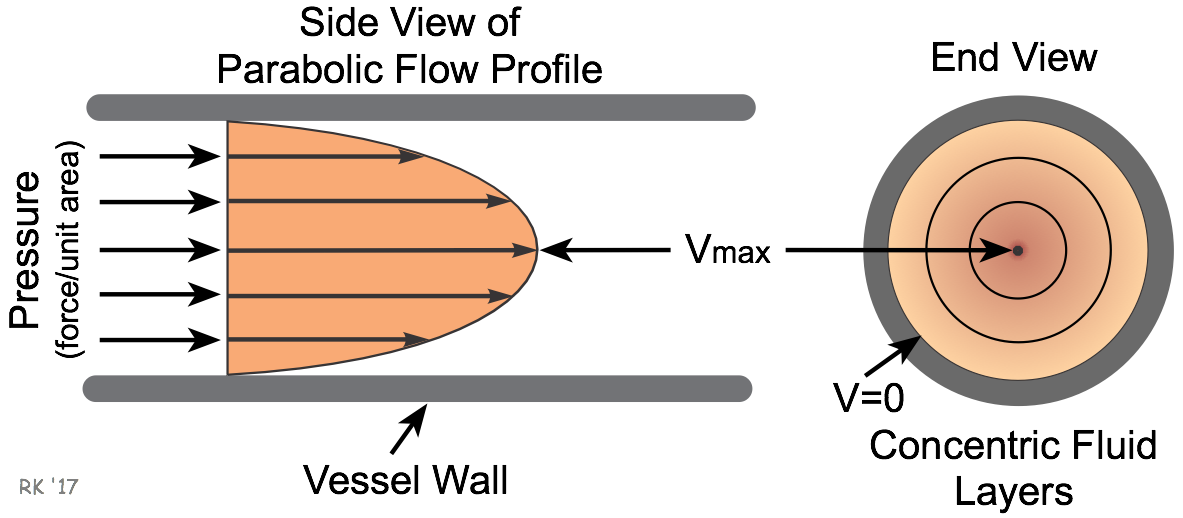
\includegraphics[width=0.7\textwidth]{figures/marco/laminar_flow.png}
    \caption{Perfil de flujo parabólico idealizado, donde la velocidad es máxima en el centro y nula en las paredes. Fuente: Tomado de \cite{klabunde_laminar}.}
    \label{fig:flujo_laminar}
\end{figure}

No obstante, el flujo sanguíneo \textit{in vivo} rara vez es estacionario, ya que su naturaleza es inherentemente pulsátil. Este fenómeno está dictado por las fases de contracción y relajación del ciclo cardíaco (sístole y diástole). Junto con la pulsatilidad, también se incorpora la compleja geometría del árbol vascular (curvaturas y bifurcaciones), generando campos de velocidades complejos que varían dinámicamente en el tiempo \cite{Ku1997}.

Capturar íntegramente esta distribución espacial de velocidades y su naturaleza pulsátil es una condición estricta, ya que esto permitirá el correcto desarrollo de algoritmos de síntesis espectral y sonificación.

\subsection{Adquisición mediante \textit{4D Flow MRI}}

La técnica \textit{4D Flow MRI} se ha consolidado como una herramienta fundamental para capturar la complejidad del flujo sanguíneo. Esta modalidad es una extensión volumétrica y temporal de la técnica convencional de resonancia magnética de contraste de fase (\textit{PC-MRI}, por sus siglas en inglés) \cite{markl2012_4dflow}.

Desde un punto de vista práctico, la base de esta modalidad se sustenta en que los protones en movimiento dentro del torrente sanguíneo experimentan un cambio en la fase de la señal de resonancia, el cual es directamente proporcional a su velocidad espacial. Para cuantificar este desplazamiento sin errores, el parámetro de adquisición más crítico es la codificación de velocidad o VENC (\textit{Velocity Encoding}). Este se define como la velocidad máxima (ya sea positiva o negativa) que puede ser registrada sin errores \cite{pineda2016_4dflow}. Si la velocidad real del flujo sanguíneo supera el VENC preestablecido, se produce un artefacto de ambigüedad conocido como \textit{aliasing} o solapamiento, el cual invierte artificialmente la dirección registrada del flujo y corrompe los datos cinemáticos. En los casos donde las velocidades fisiológicas superan el VENC configurado, es necesario repetir la adquisición con un valor mayor o aplicar técnicas de posprocesamiento para la corrección de fase (\textit{phase unwrapping}). Por consiguiente, resulta indispensable estimar a priori la velocidad máxima del vaso a estudiar para configurar adecuadamente este parámetro.

El concepto de ``cuatro dimensiones'' en la técnica \textit{4D Flow MRI} se deriva de la captura simultánea de tres dimensiones espaciales y una temporal. A diferencia del \textit{PC-MRI} bidimensional que evalúa el flujo en un único plano, esta modalidad codifica los vectores de velocidad en las tres direcciones ortogonales del espacio ($v_x, v_y, v_z$). Simultáneamente, la dimensión temporal se obtiene sincronizando la adquisición con el ciclo cardíaco del paciente mediante el electrocardiograma (ECG). Este acoplamiento divide el ciclo en múltiples intervalos temporales, permitiendo reconstruir la dinámica del flujo tridimensional a lo largo de un latido promedio representativo \cite{pineda2016_4dflow,markl2012_4dflow}.

El resultado final de este proceso es un vasto conjunto de datos discretos compuesto por tres dimensiones espaciales y una dimensión temporal. En cada vóxel (\textit{volumetric pixel}) del dominio tridimensional y para cada instante de tiempo del ciclo cardíaco, se registra la magnitud anatómica y un vector de velocidad espacial tridimensional.

Previo a cualquier análisis computacional, este volumen de datos brutos requiere una etapa de posprocesamiento mediante segmentación vascular \cite{Soulat2020}. El objetivo de este paso es aislar el vaso de interés del resto de los tejidos estáticos capturados durante la resonancia. Esto asegura que la matriz de velocidades resultante contenga exclusivamente la información hemodinámica del vaso deseado. Con este dominio aislado, los datos quedan habilitados para generar representaciones visuales tridimensionales y realizar cálculos cuantitativos sobre el flujo.

\subsection{Ultrasonido Doppler}\label{subsection:doppler_ultrasound}

El ultrasonido Doppler es una técnica de imagenología que permite evaluar la velocidad del flujo sanguíneo de forma no invasiva. Su funcionamiento se fundamenta en el efecto Doppler, un fenómeno físico caracterizado por el cambio en la frecuencia percibida de una onda cuando existe un movimiento relativo entre la fuente emisora y el receptor. En el contexto hemodinámico, un transductor piezoeléctrico emite pulsos acústicos a una frecuencia fundamental ($f_0$) hacia el interior del vaso sanguíneo. Los glóbulos rojos en movimiento actúan como partículas dispersoras (\textit{scatterers}) que reflejan estas ondas de vuelta hacia el transductor con una frecuencia alterada \cite{Poggi2024}.

La diferencia entre la frecuencia emitida y la frecuencia recibida se conoce como \textit{Doppler shift} ($f_d$) y es directamente proporcional a la velocidad de la sangre. Esta relación matemática se expresa mediante la ecuación clásica de Doppler (\ref{eq:doppler_clasica}) \cite{GOFFI2025217}:

\begin{equation}
    f_d = \frac{2 f_0 v \cos(\theta)}{c}
    \label{eq:doppler_clasica}
\end{equation}

Donde $v$ corresponde a la velocidad del flujo, $c$ representa la velocidad de propagación del sonido en los tejidos blandos, y $\theta$ es el ángulo de insonación, es decir, el ángulo formado entre el haz de ultrasonido incidente y el vector de dirección del flujo sanguíneo. La ecuación (\ref{eq:doppler_clasica}) puede ser reescrita para calcular la velocidad del flujo tal como se muestra en la ecuación (\ref{eq:velocidad_doppler}):

\begin{equation}
     v = \frac{c f_d}{2 f_0 \cos(\theta)} 
    \label{eq:velocidad_doppler}
\end{equation}

Como se estableció en \ref{sec:hemodinamica}, el flujo sanguíneo no presenta una velocidad única y homogénea, sino que se distribuye de manera parabólica y pulsa a lo largo del tiempo. Por consiguiente, el haz de ultrasonido no registra un único desplazamiento en la frecuencia, sino un espectro continuo de frecuencias superpuestas provenientes de las distintas capas del fluido. Esta multiplicidad de ecos acústicos genera lo que se conoce en el procesamiento de señales como ensanchamiento espectral (\textit{spectral broadening}) \cite{GOFFI2025217}.

Una visualización de este fenómeno se puede observar en la Figura \ref{fig:doppler_shift}, la cual expone una representación espectral donde se grafican las velocidades del flujo sanguíneo en función del tiempo.
 
\begin{figure}[H]
    \centering
    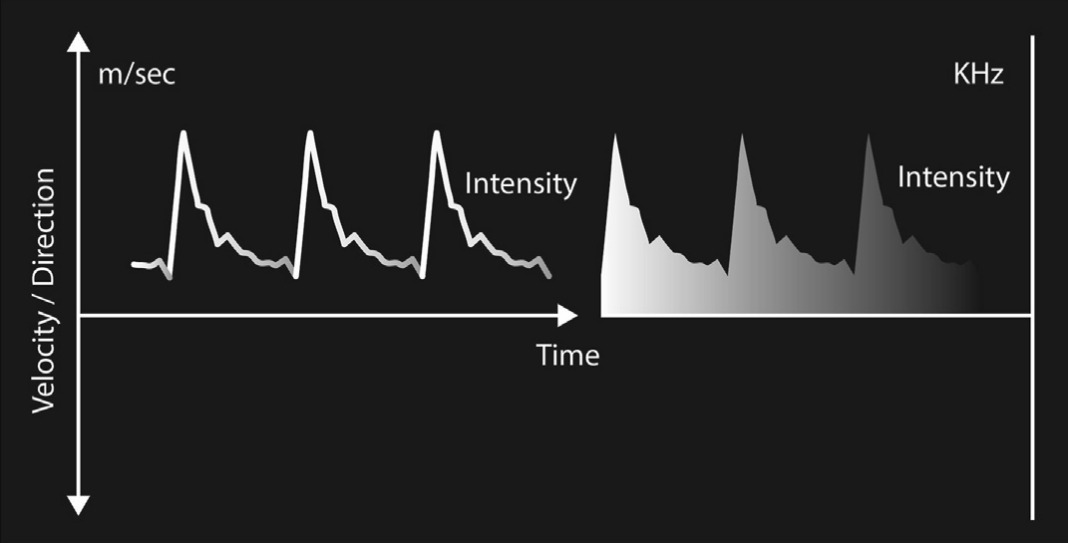
\includegraphics[width=0.7\textwidth]{figures/marco/doppler_shift.jpeg}
    \caption{Representación esquemática del desplazamiento de frecuencia (\textit{Doppler shift}) originado por los glóbulos rojos en movimiento. Fuente: Tomado de \cite{GOFFI2025217}.}
    \label{fig:doppler_shift}
\end{figure}

Una de las modalidades del ultrasonido Doppler que aplica el \textit{Doppler shift} es el \textit{Pulsed Wave Doppler} (\textit{PW-Doppler}). Esta modalidad otorga una resolución espacial, permitiendo definir una región de interés (\textit{ROI} por sus siglas en inglés) o volumen de muestra (\textit{sample volume}) a una profundidad y tamaño específico dentro del vaso sanguíneo. Al posicionar este volumen de muestra sobre el área a evaluar, el sistema es capaz de capturar los diferentes desplazamientos de frecuencia generados por los glóbulos rojos que atraviesan esta delimitación espacial. Dado que el volumen de muestra suele abarcar una región con múltiples velocidades, la señal resultante contiene el ensanchamiento espectral previamente descrito \cite{Oglat2018,GOFFI2025217}.

Para interpretar la superposición de ecos provenientes de la ROI, los sistemas de ultrasonido procesan la señal mediante análisis espectral, empleando clásicamente la Transformada Rápida de Fourier (\textit{FFT}). Este procesamiento matemático se traduce en dos salidas simultáneas: una representación gráfica continua conocida como espectrograma Doppler, y una salida acústica. Esta última ocurre de manera inherente, dado que las frecuencias del \textit{Doppler shift} fisiológico suelen coincidir con el rango de audición humana (típicamente entre 100 Hz y 8 kHz). De este modo, la señal procesada actúa como una sonificación natural que proporciona retroalimentación auditiva en tiempo real, permitiendo identificar características hemodinámicas como la pulsatilidad o la turbulencia a través del sonido \cite{hermann2011sonification}.


\subsection{Procesamiento digital de señales y mapeo de parámetros}

El procesamiento digital de señales (PDS) comprende el análisis, modificación y síntesis de señales representadas en formato discreto. En el ámbito del audio computacional, el PDS proporciona las herramientas matemáticas y algorítmicas necesarias para generar y manipular ondas sonoras a través de operaciones como la generación de osciladores, el filtrado, la modulación y la síntesis espectral \cite{dePoli1983,Moorer1977}.

Previo a la síntesis de audio es necesario que los datos hemodinámicos sean correctamente discretizados. Una forma de modelar la hemodinámica en segmentos específico de un una región vascular, es utilizando una estimación geométrica de la trayectoria principal del vaso, conocida como eje central o \textit{centerline} \cite{Antiga2008}. La extracción y visualización de las velocidades a lo largo de este \textit{centerline} permite establecer un sistema de referencia local. Evaluar planos transversales perpendiculares a este eje, permite extraer matrices que contienen la magnitud y dirección de las diferentes velocidades en cada porción del vaso. Estos son valores de entrada fundamentales para los diferentes algoritmos de PDS.

\subsubsection{Oscilador digital e integración de fase}\label{subsection:integracion_fase}

En el ámbito del procesamiento digital de señales, la generación sintética de sonido se realiza mediante osciladores digitales \cite{tierney1971digital}. Un oscilador básico produce una forma de onda periódica, siendo la onda senoidal la unidad armónica más simple. La representación matemática en tiempo discreto de una señal senoidal $s(n)$ está dada por la ecuación (\ref{eq:senoidal_discreto}):

\begin{equation}    
    s(n) = A \sin(2\pi f n T_s + \phi) 
    \label{eq:senoidal_discreto}
\end{equation}

Donde $A$ representa la amplitud máxima de la señal, $f$ es la frecuencia fundamental en hercios (Hz), $n$ es el índice de la muestra discreta, $T_s$ es el período de muestreo (el inverso de la frecuencia de muestreo $f_s$, típicamente 44100 Hz para audio de alta calidad), y $\phi$ es la fase inicial de la onda.

La ecuación (\ref{eq:senoidal_discreto}) asume un estado estacionario donde la frecuencia $f$ es constante. Por otro lado cuando la frecuencia es variante en el tiempo $f(t)$, la fase de la onda no puede expresarse como un simple producto algebraico. En su lugar, la fase instantánea $\Phi(t)$ se define matemáticamente como la integral de la frecuencia a lo largo del tiempo, esta formulación se puede observar en la ecuación (\ref{eq:integral_fase}) \cite{boashash1992estimating}:

\begin{equation}
    \Phi(t) = 2\pi \int_{0}^{t} f(\tau) d\tau
    \label{eq:integral_fase}
\end{equation}
En consecuencia, un oscilador de frecuencia variable se modela evaluando la función trigonométrica sobre esta fase acumulada ($s(t) = A \cos(\Phi(t))$). Computacionalmente, esta integración analítica se resuelve en el dominio discreto mediante métodos numéricos de integración acumulativa.

\subsubsection{Síntesis de audio}

Dado que la sangre no viaja a una velocidad única $v$, usar un solo oscilador senoidal es insuficiente. Es por esto que para replicar el comportamiento del \textit{Doppler shift}, es necesario usar técnicas más avanzadas, como se puede ver en \cite{dePoli1983} y \cite{Moorer1977}, dos de estas técnicas son:

\begin{itemize}
    \item \textbf{Síntesis aditiva:} Consiste en la suma de múltiples osciladores senoidales operando a frecuencias y amplitudes distintas. La señal resultante $S(n)$ es la sumatoria de $K$ osciladores individuales, esto se ve representado en la ecuación (\ref{eq:sumatoria_ondas}):
    \begin{equation}    
        S(n) = \sum_{k=1}^{K} A_k \sin(2\pi f_k n T_s + \phi_k) 
        \label{eq:sumatoria_ondas}
    \end{equation}
    \item \textbf{Síntesis sustractiva y modulación de ruido:} Consiste en utilizar una señal base rica en armónicos y aplicar filtros que permitan el paso de diferentes frecuencias de la señal original. Los filtros más utilizados son el filtro paso bajo (\textit{Low Pass}), paso alto (\textit{High Pass}) y paso banda (\textit{Band Pass}).
\end{itemize}

\subsubsection{Mapeo de parámetros (\textit{PMSon})}

Para implementar la sonificación, la metodología más estructurada es el Mapeo de Parámetros (\textit{PMson}, por sus siglas en inglés) \cite{hermann2011sonification}, con esto se puede establecer el enlace entre la dimensión espacial y la síntesis espectral.

La función de mapeo principal consiste en trasladar la magnitud de la velocidad calculada ($v$) hacia la frecuencia del oscilador ($f$). Esto requiere definir un rango de velocidades de entrada $[v_{min}, v_{max}]$ y mapearlo hacia un rango de frecuencias audibles $[f_{min}, f_{max}]$. Simultáneamente a este mapeo, otras propiedades cinemáticas se asignan a diferentes dimensiones acústicas para un instante de tiempo. Por ejemplo, la densidad del flujo se puede asociar directamente a la amplitud ($A$) para controlar el volumen, o la dirección del flujo a la salida del audio en un sistema stereo \cite{dubus2013systematic}.

\subsection{Estado del arte}

Contextualizar este trabajo requiere revisar el estado de la sonificación y análisis acústico en el ámbito clínico, pasando por metodologías de clasificación de sonidos del corazón, hasta modelos de sonificación personalizados, diseñados para comunicar estados de salud.

\subsubsection{Clasificación basada en características del sonido}

En la detección de enfermedades cardiovasculares, el análisis computacional del sonido del corazón se apoya en capturar su huella acústica. Una forma de realizar esto es mediante los coeficientes cepstrales de Mel (\textit{MFCC}). Esta transformación matemática traduce el audio en representaciones óptimas para evaluar sus características espaciales y temporales. Como ejemplo de su eficacia, un estudio reciente extrajo características \textit{MFCC} de sonidos del corazón para entrenar un modelo de aprendizaje profundo (\textit{CRNN}), alcanzando un 98\% de exactitud en el diagnóstico \cite{DENG202022}.

\subsubsection{Sonificación de datos multidimensionales}

En \cite{Kitaura2025}, se explora una forma de sonificación de datos multidimensionales. El estudio aborda el desafío de mapear matrices volumétricas hacia el audio, utilizando como caso de estudio la estructura tridimensional del cerebro humano mediante neuroimágenes (\textit{MRI}). El método propuesto cuantifica las correlaciones espaciales de los vóxeles aplicando estadísticas de múltiples puntos en el espacio de Fourier. Al extraer el biespectro de los datos, el algoritmo logra comprimir interacciones espaciales de alto orden y codificarlas en una señal acústica unidimensional. En la Figura \ref{fig:brain_sonification} se puede apreciar un diagrama que ilustra el método de sonificación para datos tridimensionales que utilizaron.

\begin{figure}[H]
    \centering
    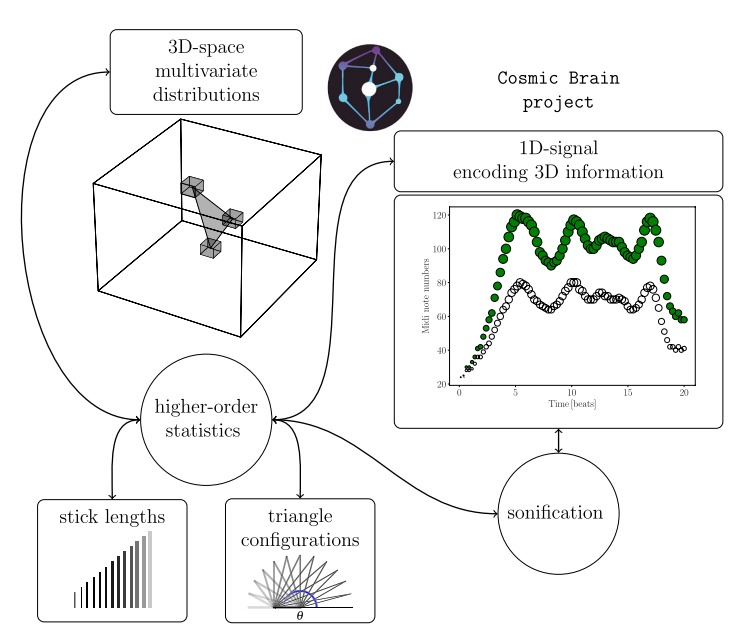
\includegraphics[width=0.8\textwidth]{figures/marco/brain_sonification.jpeg}
    \caption{Diagrama de flujo del proyecto Cosmic Brain, detallando el proceso de codificación de información 3D en una señal 1D para su sonificación. Fuente: Extraído de \cite{Kitaura2025}}
    \label{fig:brain_sonification}
\end{figure}

\subsubsection{Sonificación como alternativa a la navegación}

Otro aspecto importante de la sonificación es que ofrece vias de retroalimentación alternativas. En el trabajo realizado por \cite{Matinfar2023} investigaron la sonificación como una alternativa directa a la navegación quirúrgica visual convencional. Los autores desarrollaron un modelo de cuatro grados de libertad (\textit{4-DOF}) utilizando síntesis de modulación de frecuencia para codificar parámetros espaciales continuos. Los resultados de su estudio revelaron que traducir las métricas de alineación quirúrgica a variaciones acústicas no solo iguala la precisión clínica de las pantallas tradicionales, sino que optimiza la ergonomía cognitiva al evitar que el cirujano deba dividir su atención visual.

\subsubsection{Sonificación como modelo personalizado}
 
La sonificación se ha adaptado para comunicar métricas de salud directamente al paciente. Clark y Doryab \cite{10.1145/3570346} propusieron el uso de modelos musicales personalizados en dispositivos móviles para informar sobre el estado de bienestar del usuario. Su investigación validó que la parametrización de características sonoras, ajustadas a las preferencias individuales, permite transmitir el estado de salud de manera intuitiva y efectiva, abriendo nuevas vías para el diseño de tecnologías orientadas al cambio de comportamiento. En la Figura \ref{fig:features_sonification} se detallan los resultados de esta evaluación, ilustrando la distribución de los puntajes de bienestar (\textit{Health Score}) al ser mapeados a través de cinco dimensiones musicales distintas.

\begin{figure}[H]
    \centering
    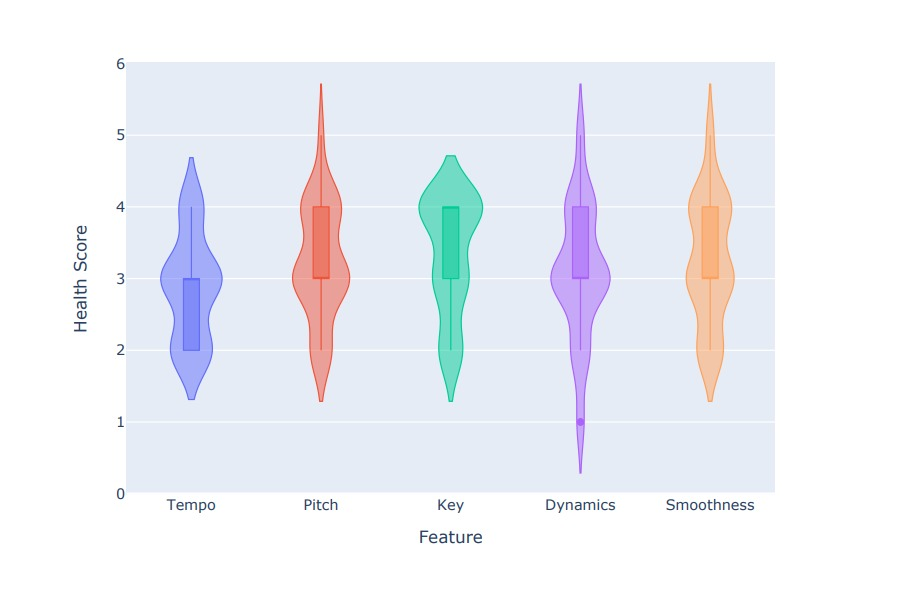
\includegraphics[width=0.8\textwidth]{figures/marco/features_sonification.jpeg}
    \caption{Distribución de puntajes (\textit{Health Score}) para distintas características de la señal acústica: Tempo, Pitch, Key, Dynamics y Smoothness. Fuente: Extraído de \cite{10.1145/3570346}}
    \label{fig:features_sonification}
\end{figure}

\subsubsection{Sonificación de \textit{4D Flow MRI}}

Como un nuevo paso en la aplicación del análisis acústico en el ámbito clínico, este trabajo presenta un modelo de sonificación desarrollado para datos de \textit{4D Flow MRI}. El enfoque principal es abordar la complejidad espacial y temporal de los datos hemodinámicos. Para lograrlo, la metodología extrae las características geométricas y cinemáticas del flujo sanguíneo para mapearlas hacia un modelo de síntesis de audio. Así, al sintetizar acústicamente los datos volumétricos de \textit{4D Flow MRI}, se entrega una nueva forma de análisis sobre estos.
\newpage
\secnumbersection{PROPUESTA DE SOLUCIÓN}\label{ch:propuesta_solucion}

El presente capítulo detalla el diseño, la estructura de la metodología y la implementación del sistema propuesto para la sonificación de datos de \textit{4D Flow MRI}. Para garantizar la escalabilidad y coherencia física de los resultados, el desarrollo de la solución no se abordó como un proceso único, sino que se fue dividido en 3 etapas, las cuales dictan la organización de este capítulo 

\begin{enumerate}
    \item \textbf{Exploración espacial y síntesis acústica:} Esta etapa está enfocada en el preprocesamiento de los datos anatómicos y su traducción acústica. Se detallan la integración del \textit{centerline}, su interpolación espacial, el cálculo iterativo de los planos de corte ortogonales y la formulación trigonométrica para extraer las proyecciones de velocidades. Además, se describe el motor de la síntesis digital de señales encargado de mapear la cinemática del fluido a parámetros sonoros. Todo el procesamiento se consolida dentro de una interfaz gráfica interactiva, la cual permite la inspección y exploración de los diferentes planos y sus flujos. 
    
    \item \textbf{Procesamiento masivo y extracción de características:} Esta segunda etapa se centra en la automatización del flujo de trabajo y la consolidación de la información. Se detalla la implementación de rutinas de procesamiento por lotes (\textit{batch processing}) para extraer y almacenar de forma masiva las proyecciones de velocidad de los diferentes casos de estudio que se ingresan al sistema. La etapa concluye con la construcción de un conjunto de datos estructurado (\textit{dataset}) mediante la extracción automatizada de descriptores correspondientes tanto a la cinemática del fluido como a la síntesis acústica.

    \item \textbf{Esquema de análisis cuantitativo y exploración interactiva:} Constituye la etapa final, destinada a corroborar la eficacia de la herramienta de sonificación. Por un lado, se establece un diseño de agrupamiento estadístico sobre el conjunto de características estructurado para analizar objetivamente la correlación de las variables. Por otro lado, se detalla la arquitectura de un tablero interactivo (\textit{dashboard}) para la exploración perceptiva, permitiendo la comparación simultánea de escenarios hemodinámicos con el fin de comprobar empíricamente si las alteraciones del flujo se traducen en firmas acústicas predecibles y distinguibles.
\end{enumerate}

\subsection{Exploración espacial y síntesis acústica}

La primera etapa del sistema se centra en el acondicionamiento de los datos y la configuración del motor de extracción espacial. El objetivo de esta fase es aislar secciones transversales del vaso sanguíneo para poder evaluar el comportamiento hemodinámico de forma iterativa y secuencial a lo largo de toda la estructura anatómica.


\subsubsection{Interpolacíon del \textit{centerline} y cálculo de planos ortogonales}

El flujo de procesamiento se inicia con la ingesta de los datos espaciales derivados de la resonancia magnética (\textit{4D Flow MRI}). Entre los datos de entrada, el sistema recibe la segmentación anatómica del vaso y una matriz de coordenadas precalculada correspondiente al \textit{centerline}.

Dado que las coordenadas originales del \textit{centerline} se encuentran expresadas en el espacio discreto de la matriz de imagen, el primer paso consiste en transformar estos datos al espacio físico real. Para ello, cada componente cartesiana de la curva se multiplica por la resolución espacial del escáner, definida por el tamaño del vóxel en sus dimensiones $X$, $Y$ y $Z$. Esta operación de escalado permite transicionar del dominio de los píxeles a una métrica en milímetros.

Una vez proyectada en el espacio físico, la curva original puede presentar un muestreo irregular para realizar un análisis continuo. Para estandarizar la topología del vaso, el sistema aplica una interpolación paramétrica mediante trazadores cúbicos (\textit{cubic splines}). Este procedimiento genera una nueva curva espacial suave, de la cual se extrae una resolución espacial de 90 puntos de estudio equidistantes. Cada coordenada interpolada $P_i = (x_i, y_i, z_i)$, con $i \in \{1, 2, \dots, 90\}$, representa el centro geométrico exacto de la región de interés para una iteración de análisis.

Para extraer de manera fidedigna la información hemodinámica en un punto de estudio $P_i$, es estrictamente necesario seccionar los volúmenes de velocidad utilizando un plano que sea perpendicular a la dirección longitudinal del vaso en ese instante específico. La orientación geométrica de este plano oblicuo queda definida por un vector normal $\vec{N}_i$. 
 
La definición de este plano ortogonal se vincula directamente con el principio físico del \textbf{ángulo de insonación} ($\theta$) descrito en el marco teórico. En ultrasonido Doppler, este ángulo —formado entre el haz acústico y la dirección del flujo sanguíneo— dicta la exactitud de la velocidad medida a través del factor de corrección $\cos(\theta)$. Al diseñar el plano de corte de manera estrictamente perpendicular a la línea central del vaso, el sistema garantiza que el vector normal $\vec{N}_i$ se mantenga paralelo a la dirección principal del flujo sanguíneo. Esta decisión de diseño equivale a establecer un escenario de exploración ideal con un ángulo de insonación computacional tendiente a $0^\circ$ ($\cos(0^\circ) = 1$), lo que maximiza los valores de \textit{Doppler shift} medidos.

Computacionalmente, este vector director se estima evaluando la derivada posicional mediante una aproximación de diferencias finitas con los puntos adyacentes de la curva interpolada:

$$\vec{N}_i = P_{i+1} - P_{i-1}$$

Donde $P_{i+1}$ y $P_{i-1}$ corresponden al punto posterior y anterior en la secuencia espacial del vaso, respectivamente. En los extremos anatómicos (el primer y el último punto), el cálculo se ajusta utilizando el punto actual y su único vecino disponible. La correcta definición del origen del plano $P_i$ y su vector normal $\vec{N}_i$ proporciona los parámetros exactos requeridos para aislar y proyectar las velocidades tridimensionales del fluido, proceso que constituye el núcleo del motor de extracción.


\subsubsection{Extracción geométrica y proyección de velocidades}

Una vez establecidos el origen del plano $P_i$ y su vector normal $\vec{N}_i$ en una iteración dada, el sistema normaliza este vector para obtener un vector director unitario $\hat{n}_i = \frac{\vec{N}_i}{||\vec{N}_i||}$. Este vector unitario es fundamental para garantizar que las transformaciones geométricas subsecuentes preserven las magnitudes físicas originales del fluido.

Con los parámetros espaciales definidos, el sistema ejecuta la sección de las matrices volumétricas correspondientes a las tres componentes espaciales de la velocidad capturadas por el resonador ($V_x$, $V_y$, $V_z$, muchas veces representadas por $V_RL$, $V_AP$ y $V_FH$). Esta se implementa mediante la extracción de un corte oblicuo (\textit{oblique slice}) a través de los volúmenes tridimensionales. La matriz bidimensional resultante contiene, en cada uno de sus píxeles, un vector de velocidad tridimensional $\vec{V} = (v_x, v_y, v_z)$ que describe el movimiento del fluido en esa región transversal específica.

Sin embargo, el realizar un corte oblicuo sobre la segmentación anatómica, la representación resultante no siempre es una región única. Con frecuencia presenta múltiples regiones aisladas o \textit{islas}. Estas discrepancias topologícas pueden ser producto de ruido inherente en la imagen, ramificaciones vasculares secundarias o vasos sanguíneos adyacentes que cruzan el mismo plano de corte.

Para aislar de manera efectiva la estructura de interés, el sistema implementa un algoritmo de etiquetado de componentes conexos (\textit{connected-component labeling}). Esta operación analiza la conectividad espacial de los píxeles y asigna una etiqueta discreta a cada agrupación independiente. A continuación, el algoritmo evalúa las propiedades geométricas de cada componente detectado —específicamente su área superficial y la distancia topológica hacia la coordenada interpolada de la línea central $P_i$—. Mediante este análisis, el sistema selecciona y extrae exclusivamente la componente conexa principal, descartando automáticamente cualquier artefacto o estructura vascular paralela.

Muchas veces los vóxeles ubicados en la periferia anatómica del vaso son altamente propensos a sufrir efectos de volumen parcial (\textit{Partial Volume Effect, PVE}), presentando una baja relación señal-ruido. Para evitar que estas mediciones introduzcan artefactos, a la región aislada se le aplica una operación de erosión que descarta las capas de píxeles más externas.

Esta nueva máscara depurada se utiliza entonces como un filtro lógico sobre las matrices de velocidad cortadas, enmascarando con valor nulo todos los píxeles fuera de la región segura. Como resultado, se obtiene una matriz tridimensional $\vec{V} = (v_x, v_y, v_z)$ que contiene vectores cinemáticos de alta fidelidad.

Sin embargo, el ultrasonido Doppler no evalúa campos vectoriales tridimensionales, sino que registra únicamente la componente de la velocidad paralela al eje de insonación. Para emular computacionalmente esta restricción física y transformar el dato volumétrico en una señal unidimensional, el sistema ejecuta un proceso de proyección ortogonal en dos etapas: aislamiento escalar y recuperación de la direccionalidad.

En primera instancia, el algoritmo calcula la proyección vectorial de la velocidad tridimensional sobre el vector normal unitario del plano. Matemáticamente, esto se formula extrayendo el vector proyectado $\vec{V}_{proj}$ y calculando su magnitud absoluta o norma euclidiana:

$$||\vec{V}_{proj}|| = ||(\vec{V} \cdot \hat{n}_i) \hat{n}_i|| = \sqrt{V_{px}^2 + V_{py}^2 + V_{pz}^2}$$


Esta magnitud $||\vec{V}_{proj}||$ representa la velocidad neta del flujo a lo largo del eje, pero carece de sentido direccional al ser un valor estrictamente positivo. Para determinar si el flujo se acerca o se aleja del plano, el sistema implementa una evaluación trigonométrica. Se calcula el cociente entre el producto escalar del vector proyectado con la normal y su magnitud absoluta, limitando el resultado al rango $[-1, 1]$ para evitar inestabilidades numéricas. Al evaluar el arcoseno de este cociente, el algoritmo extrae un factor de signo correspondiente a las orientaciones ortogonales extremas ($+90^\circ$ o $-90^\circ$).

Al normalizar este ángulo y multiplicarlo por la magnitud absoluta previa, el sistema genera la velocidad proyectada final ($V_p$). Mediante esta secuencia algorítmica y trigonométrica, se logra colapsar la complejidad del \textit{4D Flow MRI} en un perfil bidimensional, direccional y libre de ruido perimetral, estableciendo la entrada directa para el motor de sonificación.

\subsubsection{Construcción espectral y síntesis acústica}

El núcleo del sistema radica en la traducción de las velocidades proyectadas hacia el dominio auditivo y visual. El sistema emula la física detrás del ultrasonido Doppler generando un espectrograma y luego se realiza la síntesis. 

En la práctica, el espectrograma Doppler representa la distribución temporal de las velocidades del flujo. Para emular correctamente esta firma, el sistema construye una matriz espectral virtual analizando la matriz bidimensional de velocidades proyectadas a lo largo de las distintas fases del ciclo cardíaco.

El proceso se inicia definiendo dinámicamente los límites de la escala de velocidad, calculando los percentiles extremos (0.5 y 99.5) de todas las mediciones transversales para descartar valores atípicos y asegurar una representación robusta. Posteriormente, para cada fase temporal temporal, se agrupan las velocidades en un histograma continuo de 128 niveles (\textit{bins}). Este conteo captura la densidad de la sangre (cantidad de vóxeles) moviéndose a cada rango de velocidad.

Para asegurar una transición fluida en la representación visual, el algoritmo interpola las fases temporales discretas del \textit{4D Flow MRI} hacia el dominio de muestreo de audio de alta resolución mediante trazadores polinómicos (\textit{splines}). Finalmente, a la matriz resultante se le aplica una compresión no lineal mediante un factor Gamma ($\gamma = 0.65$):

$$M_{ij}' = M_{ij}^\gamma$$

Esta corrección Gamma es fundamental, ya que expande visualmente las intensidades bajas del histograma, permitiendo al observador distinguir componentes de flujo sutiles que de otro modo quedarían enmascarados por las velocidades dominantes.

Mientras que la matriz espectral gestiona la representación visual, la generación del audio se fundamenta en el principio físico del \textit{Pulsed Wave Doppler, PW}. Esto se debe a que se emula el comportamiento de una compuerta de muestra (\textit{sample volume} o \textit{gate}) al evaluar de forma aislada las velocidades contenidas en un plano transversal específico ($P_i$).

Para la síntesis acústica de esta sección espacial, el algoritmo calcula el \textit{Doppler shift} ($\Delta f$) de cada vóxel basándose en la ecuación del ultrasonido Doppler (ver Sección \ref{subsection:doppler_ultrasound}). En esta implementación, la variable $v$ corresponde a la velocidad proyectada. Asimismo, los parámetros operativos del transductor virtual se fijan en $f_0 = 1.25$ MHz para la frecuencia de emisión emulada y $c = 154,000$ cm/s para la velocidad de propagación del sonido en el tejido blando.

Una vez definido el \textit{Doppler shift} instantáneo, el sistema calcula la fase acústica acumulada integrando numéricamente la variación de la frecuencia a lo largo del tiempo del latido cardíaco (ver Sección \ref{subsection:integracion_fase}).

Finalmente, la onda acústica base de cada vóxel se genera evaluando la función coseno sobre su respectiva fase acumulada ($\cos(\Phi(t))$). Esta operación transforma la cinemática aislada de la resonancia en oscilaciones mecánicas virtuales, dejándolas listas para la consolidación del sonido final. Una vez calculadas las ondas cosenoidales individuales para cada vóxel de la región transversal, el sistema consolida el audio global del plano mediante la técnica de síntesis aditiva.

Previo a la sumatoria, el sistema implementa una espacialización dinámica basada en la dirección del flujo. Se utiliza una función tangente hiperbólica ($\tanh$) sobre las velocidades proyectadas para calcular coeficientes de ponderación estéreo. Este enfoque permite enrutar suavemente los flujos anterógrados (velocidades positivas) hacia el canal derecho y los flujos retrógrados (velocidades negativas) hacia el canal izquierdo, emulando la separación direccional presente en el \textit{hardware} de un ecógrafo real:

$$ W_{der} = 0.5 \cdot \left(1 + \tanh(v(t))\right) $$
$$ W_{izq} = 1 - W_{der} $$

La consolidación del sonido se logra multiplicando cada onda acústica individual por su respectivo peso espacial y aplicando la sumatoria a todas las componentes. Esta operación materializa la síntesis aditiva:

$$ S_{der}(t) = \sum_{i=1}^{N} \cos(\Phi_i(t)) \cdot W_{der, i} $$
$$ S_{izq}(t) = \sum_{i=1}^{N} \cos(\Phi_i(t)) \cdot W_{izq, i} $$

Previo a la etapa final de filtrado, la señal acústica debe ser moldeada para reflejar la dinámica del ciclo cardíaco. Para ello, el sistema calcula una envolvente temporal de amplitud basada en la sumatoria del flujo absoluto que atraviesa el plano transversal en cada fase. Esta curva es sometida a un suavizado gaussiano para evitar transiciones bruscas que generen clics digitales. Al multiplicar la señal de audio estéreo por esta envolvente, se garantiza que la presión sonora resultante sea directamente proporcional a la energía cinética del fluido, produciendo incrementos de volumen en sístole y atenuaciones en diástole.

Para maximizar el realismo acústico, la señal es sometida a un procesamiento final de filtrado y modulación. En primer lugar, se emula el ``golpe de pared'' (\textit{Wall Thump}), un artefacto sonoro de baja frecuencia producido por la distensión mecánica de la pared vascular durante la sístole. El algoritmo calcula la aceleración global del flujo y la utiliza para modular la amplitud de una señal estocástica grave, integrando este impacto característico al audio principal.

Finalmente, aplicando los principios de la síntesis sustractiva, las señales estéreo transitan por una etapa de filtrado digital discreto. Se implementan filtros tipo Butterworth de fase cero (\textit{filtfilt}) para esculpir la señal acústica sin introducir distorsiones de retardo temporal:

\begin{itemize}
    \item \textbf{Filtro de pared (\textit{High Pass}):} Se aplica una frecuencia de corte de 150 Hz para suprimir componentes de muy baja frecuencia.     

    \item \textbf{Filtro de paso bajo (\textit{Low Pass}):} Con una frecuencia de corte fijada en 1200 Hz, este filtro actúa como un limitador de banda para suavizar la respuesta acústica y eliminar artefactos de aliasing digital. 
\end{itemize}

El resultado de esta cadena de procesamiento algorítmico es una señal estéreo bidireccional y depurada, que recrea con alta fidelidad tanto la cinemática de los datos del \textit{4D Flow MRI} como las características sonoras del ultrasonido Doppler .

\subsubsection{Consolidación visual y exploración}

La matemática y síntesis de sonido descrita anteriormente se encapsula dentro de una interfaz gráfica de usuario, diseñada para la exploración de la estructura vascular. Este panel, ilustrado en la Figura \ref{fig:explorador_gui}, se divide en 3 visores principales sincronizados dinámicamente:

\begin{itemize}
    \item \textbf{Visor anatómico 3D:} Esta parte de la interfaz renderiza una isosuperficie (\textit{isosurface}) semi-transparente de la matriz de segmentación del vaso sanguíneo, superponiendo el \textit{centerline} interpolado. Un marcador espacial indica en tiempo real la coordenada exacta $P_i$ que está siendo procesada y su correspondiente corte oblicuo, proporcionando contexto topológico al usuario mediante un control deslizante.

    \item \textbf{Panel espectral:} Genera el espectrograma Doppler a partir de la matriz de velocidades proyectadas.
    
    \item \textbf{Panel acústico:} Grafica la forma de la onda (\textit{waveform}) de la señal de audio sintetizada.
\end{itemize}

\begin{figure}[H]
    \centering
    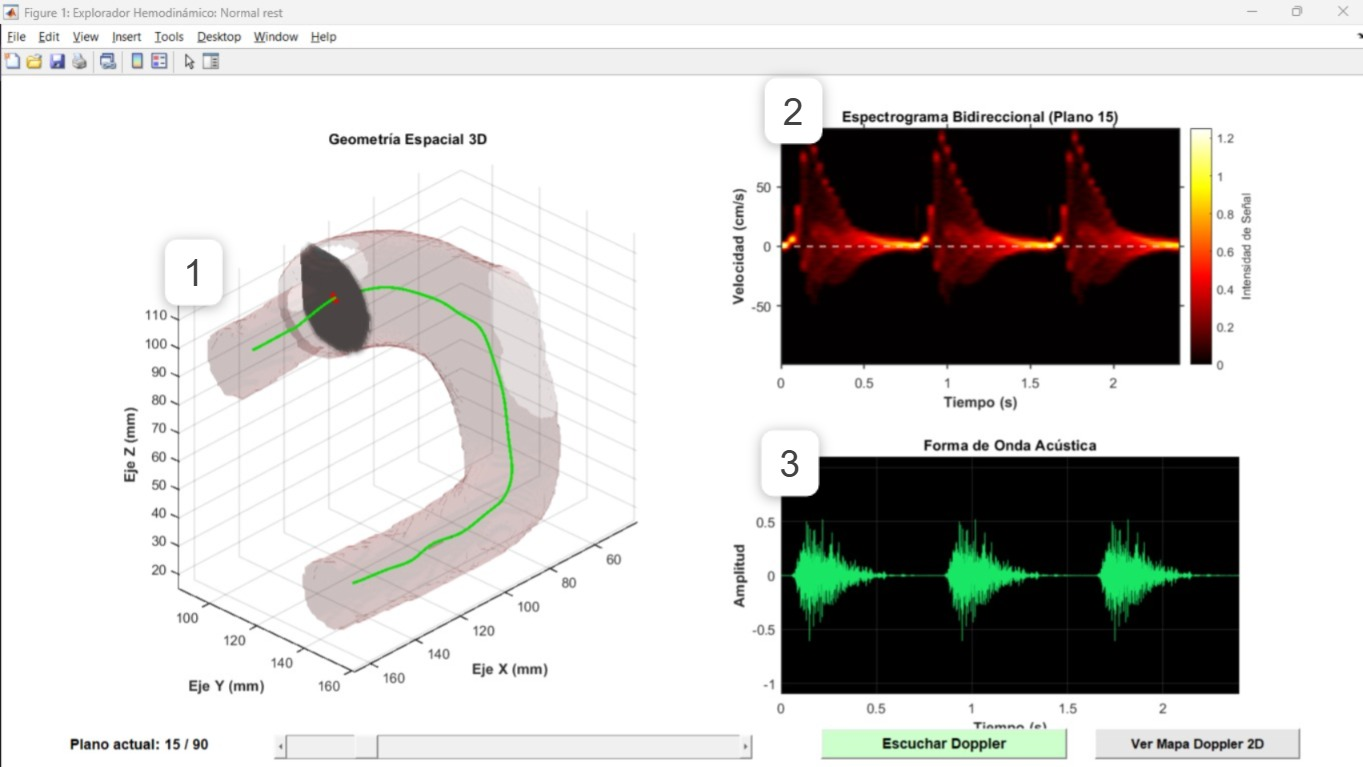
\includegraphics[width=0.9\textwidth]{figures/propuesta/explorador.jpeg}
    \caption{Interfaz del Explorador Hemodinámico: Dado un punto en el \textit{centerline} se renderiza el plano oblicuo de corte junto con la visualización anatómica (1), el panel espectral (2) y el panel acústico (3). Fuente: Elaboración propia.}
    \label{fig:explorador_gui}
\end{figure}

Adicionalmente, el sistema integra un módulo de visualización bidimensional que emula la modalidad de \textit{Color Doppler} cuyo resultado se presenta en la Figura \ref{fig:doppler_2d_gui}. A diferencia del espectrograma, que sintetiza el comportamiento dinámico del flujo en el tiempo, este módulo genera representaciones transversales para cada fase del ciclo cardíaco.

Mediante el uso de la máscara geométrica, el algoritmo proyecta las velocidades locales sobre un mapa de calor dinámico que codifica la información hemodinámica mediante una escala cromática dicotómica:
\begin{itemize}
\item \textbf{Tonalidades cálidas:} Representan el flujo anterógrado (velocidades positivas).
\item \textbf{Tonalidades frías:} Representan el flujo retrógrado (velocidades negativas).
\end{itemize}

En esta representación, la saturación del color escala proporcionalmente con la magnitud de la velocidad, permitiendo la identificación visual de gradientes hemodinámicos en la sección transversal del vaso.


\begin{figure}[H]
    \centering
    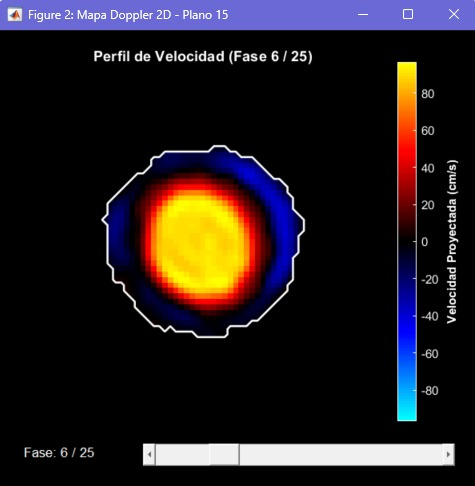
\includegraphics[width=0.65\textwidth]{figures/propuesta/doppler_2d.jpeg}
    \caption{Módulo que emula el \textit{Color Doppler} (Plano 15, Fase 6/25). Las tonalidades cálidas representan flujo anterógrado y las frías flujo retrógrado. Fuente: Elaboración propia.}
    \label{fig:doppler_2d_gui}
\end{figure}

\subsection{Procesamiento masivo y extracción de características}

La segunda etapa del desarrollo consiste en transicionar de una herramienta de exploración visual interactiva a un motor de medición automatizado. Para evaluar el impacto de diferentes morfologías y condiciones de flujo, es necesario extraer descriptores matemáticos discretos a partir de las matrices extraídas en la primera fase. Esta etapa detalla la optimización del procesamiento por lotes y la parametrización de las señales cinemáticas y acústicas.

\subsubsection{Procesamiento secuencial y gestión de memoria}

Dada la alta dimensionalidad de los volúmenes de \textit{4D Flow MRI}, la extracción manual de parámetros para las diferentes secciones transversales de cada modelo anatómico resulta inviable. Por ello, se implementó un algoritmo orquestador encargado de invocar el motor de extracción espacial de forma secuencial y autónoma para las diferentes fuentes de datos.

Durante este procesamiento masivo, el principal cuello de botella computacional es la saturación de la memoria volátil (RAM) al operar simultáneamente con múltiples matrices de gran tamaño. Para garantizar la escalabilidad, el sistema fue diseñado bajo una arquitectura de canalización (\textit{pipeline}): el orquestador ejecuta el corte y la proyección plano a plano, y exporta inmediatamente las matrices bidimensionales resultantes al almacenamiento local en formato de arreglos binarios. Este diseño transforma el modelo tridimensional pesado en un repositorio de datos ligero y fragmentado, permitiendo el procesamiento ininterrumpido sin comprometer la estabilidad del sistema computacional.

\subsubsection{Parametrización cinemática y acústica (\textit{Feature Extraction})}

Con las señales espaciales exportadas, el sistema ejecuta un módulo de parametrización encargado de traducir los campos vectoriales y las ondas de sonido en métricas escalares concretas. Para garantizar una comparación coherente a lo largo de toda la estructura, el sistema implementa una sincronización temporal dinámica basada en el caudal volumétrico.

Computacionalmente, la integración espacial del campo de velocidades se ejecuta mediante una sumatoria discreta de las magnitudes absolutas de todos los vóxeles válidos para cada fase temporal $t$:

$$ Q(t) = \sum_{j=1}^{N} |v_j(t)| $$

Donde $N$ es el número total de vóxeles que conforman el lumen en el plano transversal analizado, y $v_j(t)$ es la velocidad proyectada de cada vóxel. La utilización del valor absoluto en esta formulación es una consideración fundamental: garantiza que la presencia de flujos retrógrados o vórtices locales sumen a la energía cinética total de la sección en lugar de cancelarse matemáticamente con el flujo anterógrado.

Una vez construido el vector de caudal $Q(t)$ para todo el ciclo cardíaco, el algoritmo identifica el instante donde se alcanza el máximo valor del ciclo ($t_{sistole} = \arg\max Q(t)$). La fase temporal que satisface esta condición es etiquetada como el pico sistólico, estableciendo el punto de medición estándar para la extracción de características estáticas.

La extracción de parámetros se divide en dos dominios complementarios:

\textbf{Métricas de la dinámica de fluidos:} Estos parámetros cuantifican la física del flujo a partir de la cinemática volumétrica del latido:
\begin{itemize}
    \item \textbf{Velocidad máxima ($V_{max}$) y media ($V_{mean}$):} La velocidad máxima se obtiene utilizando el percentil 99.5 de la distribución de velocidades del plano en el pico sistólico. La aplicación de este límite probabilístico, en lugar del valor máximo absoluto, es una contramedida algorítmica para mitigar el impacto de valores anómalos (\textit{outliers}) propios del ruido de la resonancia.
    
    \item \textbf{Varianza y asimetría espacial (\textit{Skewness}):} Describen estadísticamente la distribución de los gradientes de velocidad transversal. Valores elevados indican una alteración del perfil parabólico normal, caracterizando la pérdida de laminaridad, flujos caóticos o zonas de recirculación.
    
    \item \textbf{Índice de pulsatilidad (PI):} Parámetro hemodinámico clásico calculado a partir de la evolución temporal de todo el ciclo cardíaco, relacionando la amplitud de la velocidad (sístole menos diástole) con la velocidad media del ciclo.
\end{itemize}

\textbf{Métricas de la señal digital:} Aprovechando el motor de síntesis, las proyecciones espaciales se transforman en señales de audio. Para estandarizar el análisis, la señal es truncada a una ventana de observación correspondiente a exactamente un ciclo cardíaco. Sobre esta onda modulada se extraen los siguientes descriptores de audio digital:
\begin{itemize}
    \item \textbf{Análisis en el dominio del tiempo:} Se calcula la energía cuadrática media (\textit{RMS}) y la tasa de cruces por cero (\textit{Zero-Crossing Rate, ZCR}). Estas variables traducen la presión sonora aparente y la densidad de fluctuaciones de la señal acústica\cite{eronen2000musical}.
    
    \item \textbf{Análisis en el dominio de la frecuencia:} Mediante la Transformada Rápida de Fourier (FFT), se proyecta la señal sonora a su espectro de frecuencias para derivar su Centroide Espectral y su Dispersión Espectral (\textit{Spectral Spread}). Estas variables modelan matemáticamente el ensanchamiento espectral (\textit{Spectral Broadening}).
    
    \item \textbf{Coeficientes Cepstrales en las Frecuencias de Mel (MFCC 1 al 3):} Descriptores fundamentales en el reconocimiento de patrones sonoros. Al aplicar un banco de filtros espaciados según la escala Mel, se modela la resolución no lineal de la audición humana. La extracción de estos coeficientes permite cuantificar el ``timbre'' del flujo\cite{zheng2015heart}.
\end{itemize}

La extracción sistemática de estas métricas genera una matriz de datos que unifica las características cinemáticas del flujo con su firma acústica, esta matriz representa un conjunto de datos estructurados o \textit{dataset}.

\subsection{Esquema de análisis cuantitativo y exploración interactiva}

La etapa final consiste en establecer el esquema de evaluación sobre el espacio de características multimodal. Con este fin, se desarrolla una herramienta de análisis comparativo interactiva. El objetivo de esta implementación es contar con un mecanismo objetivo para comprobar si la traducción cinemática-acústica es efectiva, y evidenciar si las alteraciones del flujo sanguíneo generan, bajo los criterios de sonificación establecidos, firmas sonoras predecibles y distinguibles.

\subsubsection{Agrupamiento estadístico y análisis de importancia}


Para evaluar matemáticamente la capacidad de discriminación del \textit{dataset} construido, se implementa una etapa de aprendizaje automático no supervisado. El análisis se aborda mediante la ejecución del algoritmo de agrupamiento $K$-Means, configurado para particionar los datos en $k$ clústeres. Con el fin de aislar el peso predictivo de cada dominio, el agrupamiento se itera sobre tres subconjuntos independientes: un espacio estrictamente cinemático, un espacio puramente acústico y el espacio multimodal fusionado

La validación de los clústeres descubiertos se estructura en dos niveles. A nivel interno, se cuantifica la cohesión y separación de los grupos utilizando el coeficiente de \textit{Silhouette} y el índice de Calinski-Harabasz. A nivel externo, se generan tablas de contingencia (\textit{cross-tables}) que cruzan las asignaciones del algoritmo con los metadatos inherentes a cada registro, es decir, el identificador del modelo físico y la condición de flujo simulada. Este cruce permite evaluar si las agrupaciones descubiertas logran segmentar de forma natural los diferentes escenarios clínicos abordados.

Adicionalmente, para comprender la contribución de cada variable en la formación de estos patrones, se aplica un Análisis de Componentes Principales (PCA). La extracción de los pesos absolutos del primer componente principal ($PC_1$) permite identificar cuáles descriptores actúan como los marcadores de varianza más fuertes dentro del modelo no supervisado.

% \subsubsection{Entorno interactivo de evaluación clínica}

% El segundo frente del esquema de evaluación, orientado a la percepción cualitativa, consiste en el despliegue del \textit{Dashboard Hemodinámico Interactivo}. Esta interfaz se vincula de forma directa con la primera etapa de la metodología, al heredar la reconstrucción geométrica tridimensional del vaso y la discretización espacial de los 90 planos transversales. Asimismo, la herramienta representa un aprovechamiento integral del motor de síntesis desarrollado en la segunda etapa, explotando la emulación computacional del ultrasonido Doppler para transformar instantáneamente las métricas cinemáticas locales en señales sonoras. Su diseño está concebido para realizar pruebas comparativas simultáneas (\textit{A/B testing}) entre distintos escenarios anatómicos o estados de flujo.

% Para articular analíticamente esta integración, el entorno dual sincroniza las siguientes dimensiones operativas:
% \begin{itemize}
%     \item \textbf{Navegación y control espacial (Vínculo con Etapa 1):} Utiliza el renderizado tridimensional de la isosuperficie del vaso y su eje central (\textit{centerline}) para permitir al usuario desplazar un marcador interactivo a lo largo de los puntos de estudio equidistantes ($P_i$). Esto permite seleccionar con precisión anatómica la sección transversal exacta que se desea evaluar.
%     \item \textbf{Procesamiento y audición bajo demanda (Aprovechamiento de Etapa 2):} Al posicionar el marcador en un plano específico, el sistema extrae automáticamente el vector de características cinemáticas y activa las rutinas de síntesis acústica. Esto genera e invoca de manera inmediata la sonificación estéreo basada en el comportamiento local del fluido.
%     \item \textbf{Representación visual de las señales:} Despliega bidireccionalmente las matrices de densidad espectral (espectrogramas) y las formas de onda en el dominio del tiempo resultantes de la síntesis, autoescalando los ejes paramétricos para garantizar una comparación visual y acústica coherente entre ambos casos estudiados.
% \end{itemize}

% El significado metodológico de este comparador interactivo radica en su capacidad para unificar los hallazgos de las fases previas en una experiencia analítica unificada. Al enlazar la ubicación espacial exacta determinada en la Etapa 1 con la respuesta acústica simulada en la Etapa 2, la interfaz proporciona un mecanismo objetivo y multisensorial para comprobar si los criterios de sonificación establecidos logran traducir de manera efectiva las anomalías hemodinámicas en firmas sonoras clínica y perceptivamente distinguibles.



\newpage
\section{VALIDACIÓN DE LA SOLUCIÓN}

El presente capítulo tiene como objetivo fundamental comprobar la eficacia de la solución metodológica y tecnológica propuesta. Para someter el sistema a una prueba rigurosa, se estableció un marco experimental basado en el procesamiento de adquisiciones controladas de resonancia magnética. 

La demostración empírica de la propuesta se divide en dos ejes principales de evaluación:

\begin{itemize}
    \item \textbf{Verificación del procesamiento espacial y acústico (Etapas \ref{item:etapa1} y \ref{item:etapa2}):} Consiste en verificar el correcto desempeño operativo de los módulos de \textit{software}. Se analizan los resultados de la adaptación espacial y de la síntesis de audio, corroborando que el sistema logra aislar la anatomía del fantoma y transformar exitosamente su cinemática en señales sonoras y espectrogramas representativos.

    
    \item \textbf{Validación estadística y perceptiva (Etapa 3):} Se centra en la comparación y capacidad discriminatoria del modelo sobre los datos generados. Inicia con un análisis cuantitativo apoyado en técnicas de aprendizaje no supervisado para medir la separación estadística de las métricas. Culmina con una validación cualitativa en el entorno interactivo, demostrando que el contraste de estas sonificaciones permite identificar firmas acústicas distinguibles frente a variaciones del flujo.
\end{itemize}


\subsection{Caracterización de los datos experimentales}

Previa a la exposición de los resultados, es necesario detallar las características del conjunto de datos de prueba utilizado. El marco experimental está compuesto por adquisiciones de \textit{4D Flow MRI} correspondientes a fantomas cardiovasculares. En el ámbito de la hemodinámica, un fantoma es un modelo físico calibrado diseñado específicamente para emular la geometría del sistema cardiovascular.

Para evaluar la capacidad de respuesta del sistema ante alteraciones complejas, el conjunto de pruebas contempló modelos con distintos grados de coartación, un estrechamiento anatómico del vaso que obliga al fluido a acelerarse abruptamente y generar turbulencia. Al procesar diferentes diámetros para esta lesión, se busca verificar si el algoritmo logra capturar y parametrizar acústicamente los diferentes escenarios.

Para comprobar que el modelo acústico es capaz de distinguir diferentes niveles de intensidad hemodinámica, las geometrías fueron sometidas a dos condiciones de flujo contrastantes:

\begin{itemize}
    \item \textbf{Condición de reposo (\textit{rest}):} Emula el comportamiento fisiológico basal, definiendo un patrón de velocidades no alterado por factores externos.
    
    \item \textbf{Condición de estrés (\textit{stress}):} Representa un estado de alta demanda cardiovascular, el cual fuerza un aumento drástico en las velocidades en el flujo.
\end{itemize}

Las configuraciones que definen los escenarios de estudio evaluados se resumen en la Tabla \ref{table:casos_estudio}.

\begin{table}[h]
    \centering
    \caption{\label{table:casos_estudio} Conjunto de datos evaluados en la experimentación.}
    \begin{tabular}{|l|l|}
        \hline
        \textbf{Geometría del Fantoma} & \textbf{Condiciones Evaluadas} \\
        \hline
        Normal & Reposo (\textit{rest}), Estrés (\textit{stress}) \\
        \hline
        13 mm & Reposo (\textit{rest}), Estrés (\textit{stress}) \\
        \hline
        11 mm & Reposo (\textit{rest}), Estrés (\textit{stress}) \\
        \hline
        9 mm & Reposo (\textit{rest}), Estrés (\textit{stress}) \\
        \hline
    \end{tabular}
\end{table}


Definidos los ocho escenarios de estudio, la primera fase de validación aborda el desempeño de los módulos de procesamiento espacial y acústico. Considerando que los volúmenes hemodinámicos, las segmentaciones y los \textit{centerlines} se proporcionan como datos de entrada, el objetivo de esta etapa es demostrar la correcta integración y transformación de estos elementos. A continuación, se verifica la capacidad del algoritmo para iterar sobre la trayectoria anatómica y extraer los perfiles de velocidad locales, para finalmente exhibir cómo esta cinemática se convierte exitosamente en las señales sonoras y espectrogramas representativos del fantoma.


\subsection{Verificación del procesamiento espacial y acústico}

La verificación de este flujo de trabajo se expone en dos partes. Primero, se analiza el desempeño del algoritmo base (Etapa \ref{item:etapa1}), demostrando cómo el sistema es capaz de integrar la anatomía, extraer la cinemática del fluido y sintetizar su respectivo audio. Segundo, se documenta la automatización del proceso (Etapa \ref{item:etapa2}), confirmando que el código logró procesar con éxito la totalidad de los escenarios de prueba.

\subsubsection{Validación de la reconstrucción geómetrica}

El paso inicial en la ejecución del flujo de trabajo consistió en corroborar la correcta lectura e integración de los datos anatómicos de entrada. El módulo de procesamiento arranca con la ingesta de la segmentación volumétrica del vaso y proyectando espacialmente su respectivo \textit{centerline}. 

Una vez asimilada la estructura anatómica, la discretización de la línea central se ejecuta utilizando la rutina \textit{interparc}\footnote{\url{https://la.mathworks.com/matlabcentral/fileexchange/34874-interparc}}. Este procedimiento subdivide el \textit{centerline} en un conjunto de coordenadas espacialmente equidistantes. Como producto directo de esta discretización, el algoritmo logra calcular los vectores normales locales y generar, en cada iteración, los planos transversales ortogonales a la dirección del vaso. Verificar la correcta proyección de estos planos es un paso obligatorio, ya que sobre ellos se aislarán posteriormente las velocidades locales.

La Figura \ref{fig:geometrias_fantomas} muestra la salida visual de este procesamiento espacial, contrastando un modelo sano con uno patológico.

\begin{figure}[h]
    \centering
    \begin{subfigure}{0.48\textwidth}
        \centering
        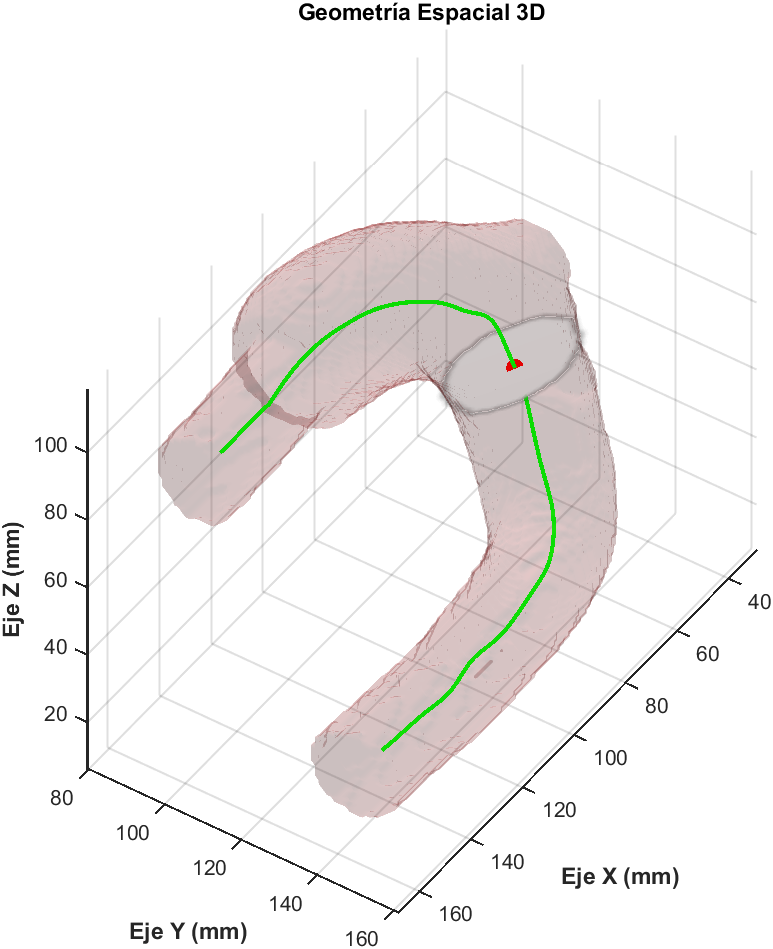
\includegraphics[width=\linewidth]{figures/validacion/fase1/geometria_normal_p45.png}
        \caption{Fantoma normal (Plano 45)}
        \label{fig:geo_normal}
    \end{subfigure}\hfill
    \begin{subfigure}{0.48\textwidth}
        \centering
        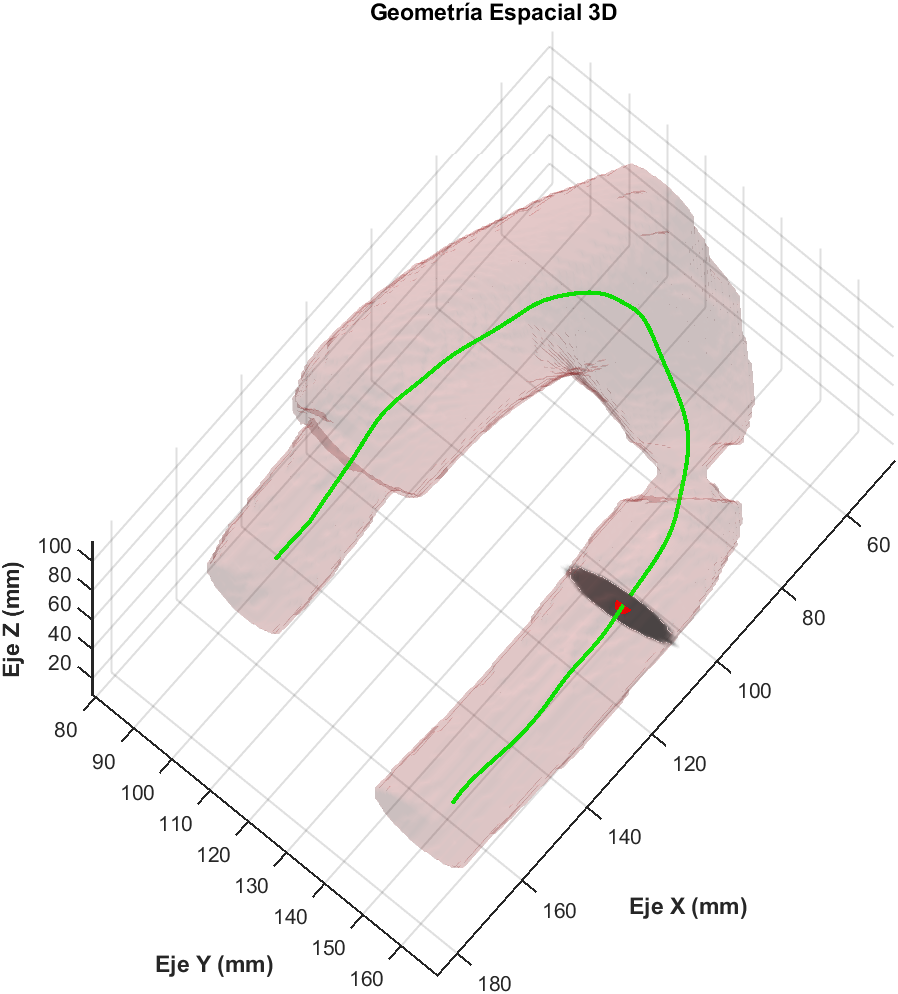
\includegraphics[width=\linewidth]{figures/validacion/fase1/geometria_9mm_p70.png}
        \caption{Fantoma 9 mm (Plano 70)}
        \label{fig:geo_9mm}
    \end{subfigure}
    \caption{Representación espacial tridimensional generada por el sistema. Se evidencia la generación de la isosuperficie, el \textit{centerline} (verde) y el plano transversal de discretización en su respectiva iteración. Destaca la clara captura del estrechamiento en la zona de coartación (b). Fuente: Elaboración propia.}\label{fig:geometrias_fantomas}
\end{figure}

Como se observa en la representación gráfica, el sistema logra integrar la isosuperficie con la discretización del \textit{centerline}, proyectando los planos de corte de manera precisa. La comparación visual confirma la captura de los cambios morfológicos entre fantomas, evidenciando la caída abrupta de diámetro del fantoma con coartación frente a la continuidad del vaso sano.


\subsubsection{Validación de la síntesis acústica y análisis espectral}

Una vez validada la discretización del \textit{centerline}, el flujo de trabajo procede con la proyección de las velocidadades y su transformación en señales sonoras. El objetivo en esta instancia es corroborar que el motor de emulación es capaz de procesar la cinemática aislada y generar exitosamente la síntesis acústica y espectrales.

Para evidenciar la correcta ejecución de esta etapa, la Figura \ref{fig:sintesis_acustica} expone las salidas generadas por el \textit{software} para el fantoma normal (plano 45) y el fantoma con coartación de 9 mm (plano 70).

\begin{figure}[H]
    \centering
    % Fila 1: Espectrogramas
    \begin{subfigure}{0.48\textwidth}
        \centering
        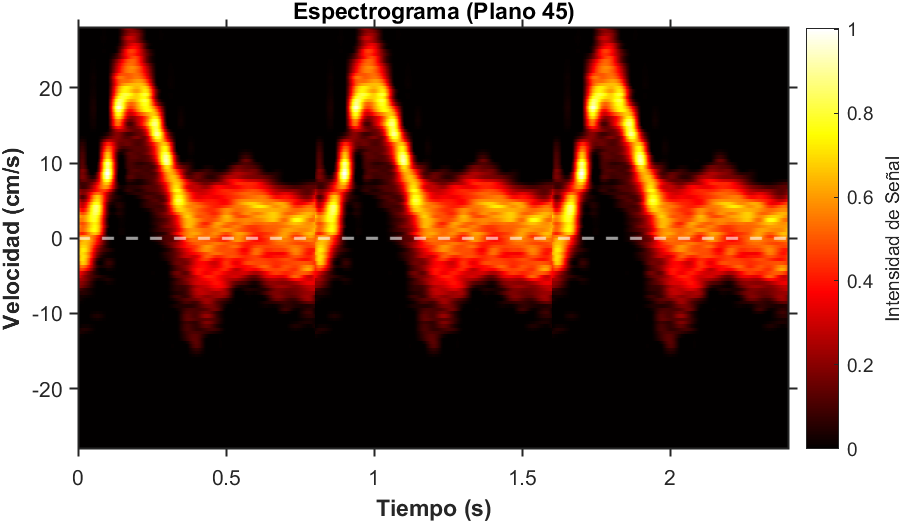
\includegraphics[width=\linewidth]{figures/validacion/fase1/gn_espectro_p45.png}
        \caption{Espectrograma - Fantoma normal}
        \label{fig:spec_normal}
    \end{subfigure}\hfill
    \begin{subfigure}{0.48\textwidth}
        \centering
        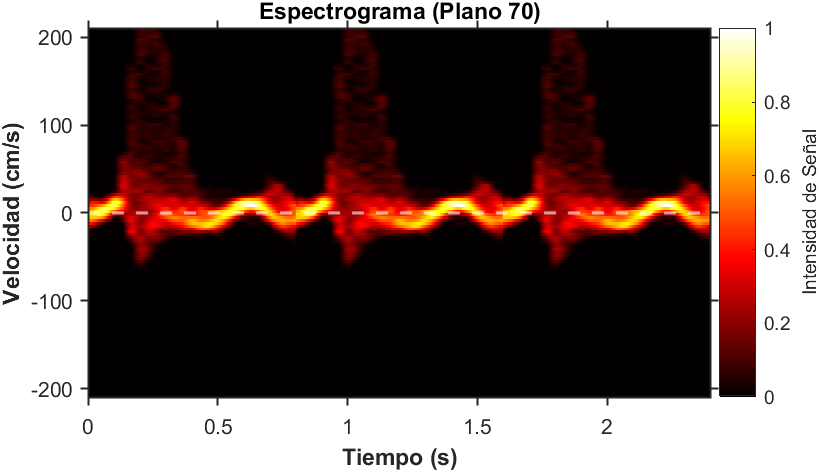
\includegraphics[width=\linewidth]{figures/validacion/fase1/g9_espectro_p70.png}
        \caption{Espectrograma - Fantoma 9 mm}
        \label{fig:spec_9mm}
    \end{subfigure}
    
    \vspace{0.5cm} % Espacio entre filas
    
    % Fila 2: Formas de Onda
    \begin{subfigure}{0.48\textwidth}
        \centering
        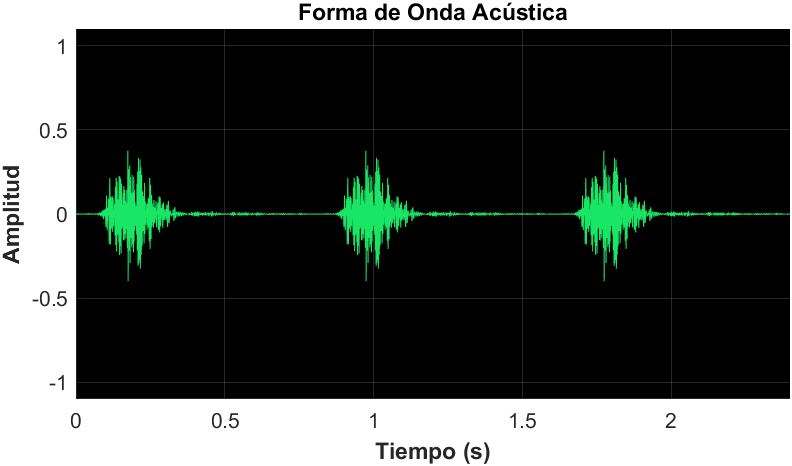
\includegraphics[width=\linewidth]{figures/validacion/fase1/gn_sonido_p45.png}
        \caption{Onda acústica - Fantoma normal (a)}
        \label{fig:onda_normal}
    \end{subfigure}\hfill
    \begin{subfigure}{0.48\textwidth}
        \centering
        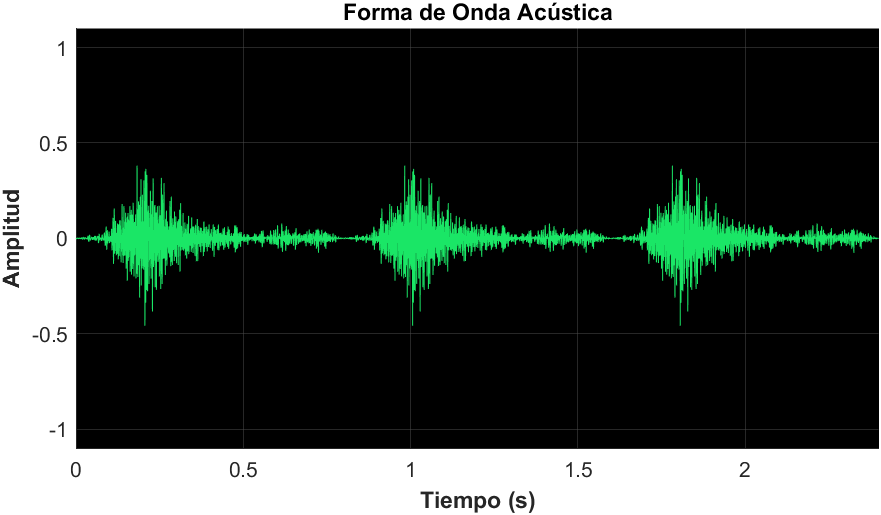
\includegraphics[width=\linewidth]{figures/validacion/fase1/g9_sonido_p70.png}
        \caption{Onda acústica - Fantoma 9 mm (b)}
        \label{fig:onda_9mm}
    \end{subfigure}
    \caption{\label{fig:sintesis_acustica} Espectrograma y onda acústica en condición de reposo (\textit{rest}) para diferentes escenarios morfológicos y topológicos. Fuente: Elaboración propia.}
\end{figure}

Como se observa en los resultados, el sistema logra extraer la información de los planos de corte y traducirla en archivos acústicos y gráficos estructurados. La clara diferencia en las escalas y amplitudes registradas entre ambos modelos confirma que el algoritmo de síntesis responde a los distintos perfiles de velocidad del \textit{4D Flow MRI}, comprobando el correcto desempeño operativo del módulo base. Para complementar esta validación visual, es posible acceder a la reproducción de las señales generadas mediante los siguientes enlaces: \href{https://drive.google.com/file/d/1xQmC3SaCplyq4cFz9ADJMwVXydT0yq6e/view?usp=sharing}{salida acústica del fantoma normal (a)} y \href{https://drive.google.com/file/d/1KgReb6jlhsudJGxGEyWbSvPVMoqxSP4G/view?usp=sharing}{salida acústica del fantoma de 9 mm (b)}.

Complementando la validación espectral y sonora, es necesario comprobar la correcta ejecución del módulo de emulación del \textit{Color Doppler}. Este componente es sirve para corroborar que el algoritmo proyecta adecuadamente los vectores de velocidad de forma dinámica, respondiendo a la evolución fisiológica del ciclo cardíaco sin introducir artefactos topológicos.

A fin de ilustrar esta capacidad, la Figura \ref{fig:validacion_doppler2d_temporal} detalla el mapeo bidimensional de velocidades para el fantoma sin estenosis (Normal) en condición \textit{rest}. La evaluación se focaliza en el plano transversal 45, zona anatómica representativa de la porción central del conducto. Al desplegar esta proyección en cuatro fases discretas del ciclo cardíaco, es posible visualizar la evolución de las proyecciones generadas.

\begin{figure}[H]
    \centering
    % Fila 1
    \begin{subfigure}{0.48\textwidth}
        \centering
        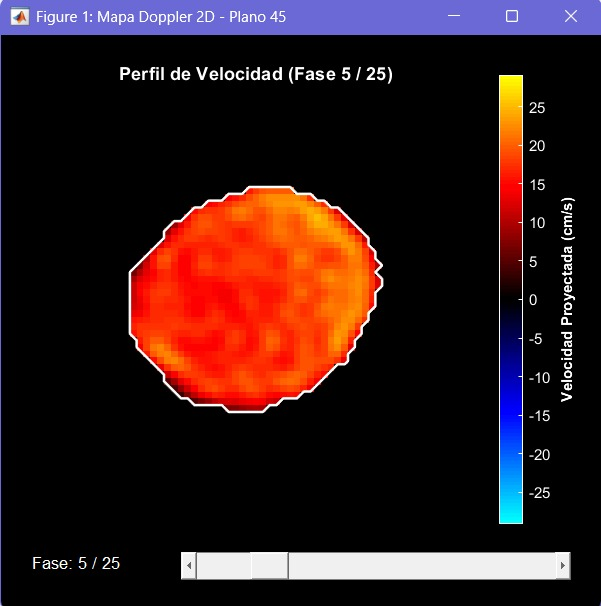
\includegraphics[width=\linewidth]{figures/validacion/fase1/gn_2d_p45_fase5.jpeg} 
        \caption{Fase 5}
        \label{fig:mapa2d_f5}
    \end{subfigure}\hfill
    \begin{subfigure}{0.48\textwidth}
        \centering
        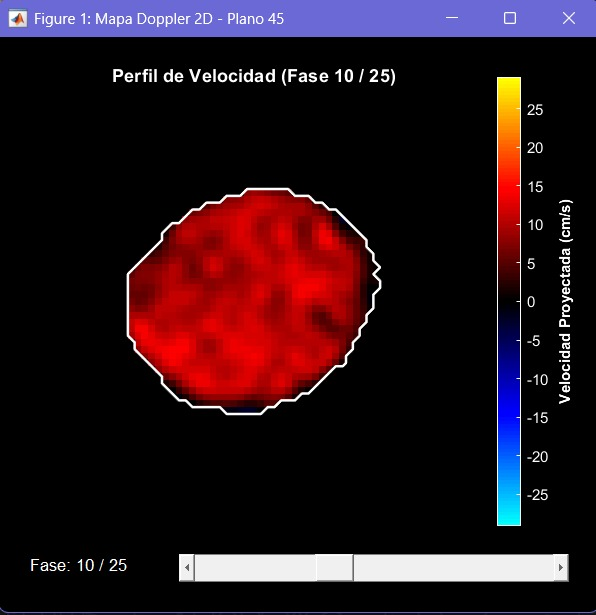
\includegraphics[width=\linewidth]{figures/validacion/fase1/gn_2d_p45_fase10.jpeg} 
        \caption{Fase 10}
        \label{fig:mapa2d_f10}
    \end{subfigure}
    
    \vspace{0.5cm} % Espacio entre filas
    
    % Fila 2
    \begin{subfigure}{0.48\textwidth}
        \centering
        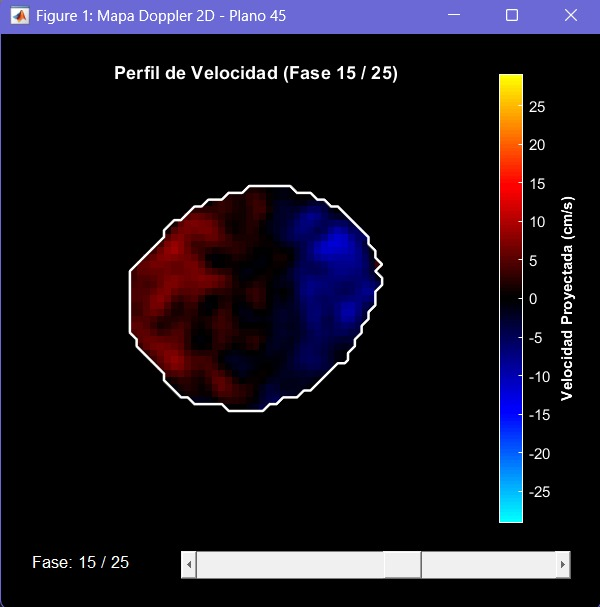
\includegraphics[width=\linewidth]{figures/validacion/fase1/gn_2d_p45_fase15.jpeg} 
        \caption{Fase 15}
        \label{fig:mapa2d_f15}
    \end{subfigure}\hfill
    \begin{subfigure}{0.48\textwidth}
        \centering
        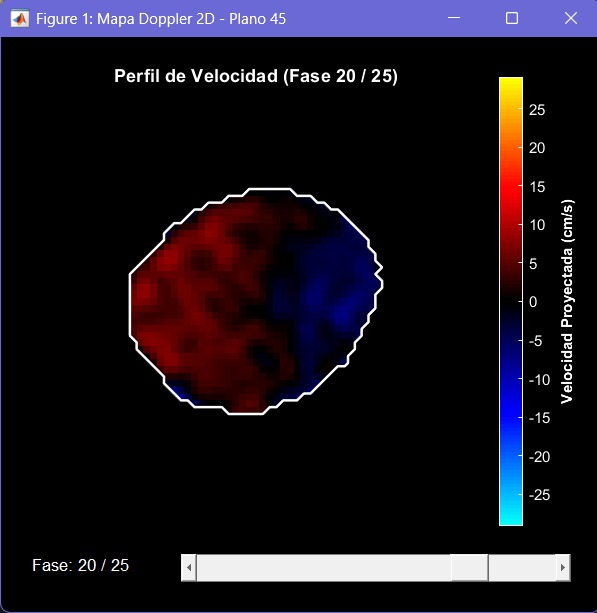
\includegraphics[width=\linewidth]{figures/validacion/fase1/gn_2d_p45_fase20.jpeg} 
        \caption{Fase 20}
        \label{fig:mapa2d_f20}
    \end{subfigure}
    \caption{\label{fig:validacion_doppler2d_temporal} Evolución temporal del \textit{Color Doppler} virtual en el plano 45 del fantoma Normal. Fuente: Elaboración propia.}
\end{figure}

Como se aprecia en la secuencia visual, el sistema aísla exitosamente el plano transversal que atraviesa el vaso, conteniendo exclusivamente los perfiles hemodinámicos de la región de interés. 

En síntesis, el sistema ha demostrado su capacidad para procesar la complejidad de los datos provenientes del \textit{4D Flow MRI}, logrando aislar topológicamente el vaso y traducir su cinemática en representaciones acústicas, espectrales y espaciales consistentes entre sí. No obstante, aunque esta herramienta resulta fundamental para una primera inspección cualitativa, el análisis comparativo entre múltiples morfologías y secciones transversales exige un enfoque paramétrico y escalable. Por consiguiente, la siguiente etapa de validación abordará la segunda fase de la investigación, comprobando cómo este núcleo de procesamiento fue automatizado para extraer, de forma masiva, los descriptores numéricos que caracterizan la hemodinámica de todos los modelos de estudio.


% \subsubsection{Validación de la extracción paramétrica y procesamiento masivo}

% Tras comprobar la fidelidad espacial y acústica del motor base, la validación de la segunda etapa se enfoca estrictamente en verificar el correcto desempeño computacional del algoritmo de procesamiento por lotes (\textit{batch processing}) y la integridad estructural de los datos exportados. El objetivo de esta fase fue procesar de forma ininterrumpida las matrices correspondientes a los diferentes escenarios hemodinámicos para consolidar exitosamente un espacio de características multidimensional, garantizando que el sistema operara de manera autónoma sin pérdida de información.

% El procesamiento continuo de los 8 modelos de estudio (condiciones de reposo y estrés) permitió evaluar un total de 720 secciones transversales anatómicas. Durante la ejecución de esta etapa, la inspección del repositorio intermedio expuso una varianza empírica significativa en la huella de almacenamiento de los archivos. Lejos de representar una anomalía computacional, esta fluctuación constituye una validación geométrica intrínseca: el peso de cada archivo es directamente proporcional al área anatómica de la sección transversal del lumen vascular. Planos amplios contienen un mayor número de vóxeles catalogados como flujo, generando matrices más pesadas, mientras que las zonas estrechas o de coartación producen arreglos sustancialmente más ligeros. Esta correspondencia demuestra que el sistema aísla y se adapta dinámicamente a la morfología real del vaso iteración tras iteración.

% En cuanto a la arquitectura de datos, el diseño computacional priorizó la máxima fidelidad matemática. Durante las etapas preliminares, el sistema operaba los tensores en precisión simple (\textit{single}, 32 bits) para minimizar el impacto en la memoria. No obstante, para evitar errores de truncamiento acumulativos durante la integración de las señales acústicas y el cómputo del espectro de Fourier, se determinó escalar y fijar el procesamiento a precisión doble (\textit{double}, 64 bits). 

% Evidentemente, esta exigencia matemática duplicaba la carga sobre la memoria volátil. Para mitigar este cuello de botella y evitar la saturación de la memoria RAM, se implementó la arquitectura de canalización que exporta de manera fragmentada las matrices de cada plano hacia el almacenamiento local en archivos binarios (\textit{.mat}). Para evidenciar el impacto de esta decisión de ingeniería y la carga que el sistema logró gestionar exitosamente, la Figura \ref{fig:exportacion_batch_precision} contrasta la huella de memoria entre la precisión base y la implementación final de alta resolución.

% \begin{figure}[H]
%     \centering
%     \begin{subfigure}{0.85\textwidth}
%         \centering
%         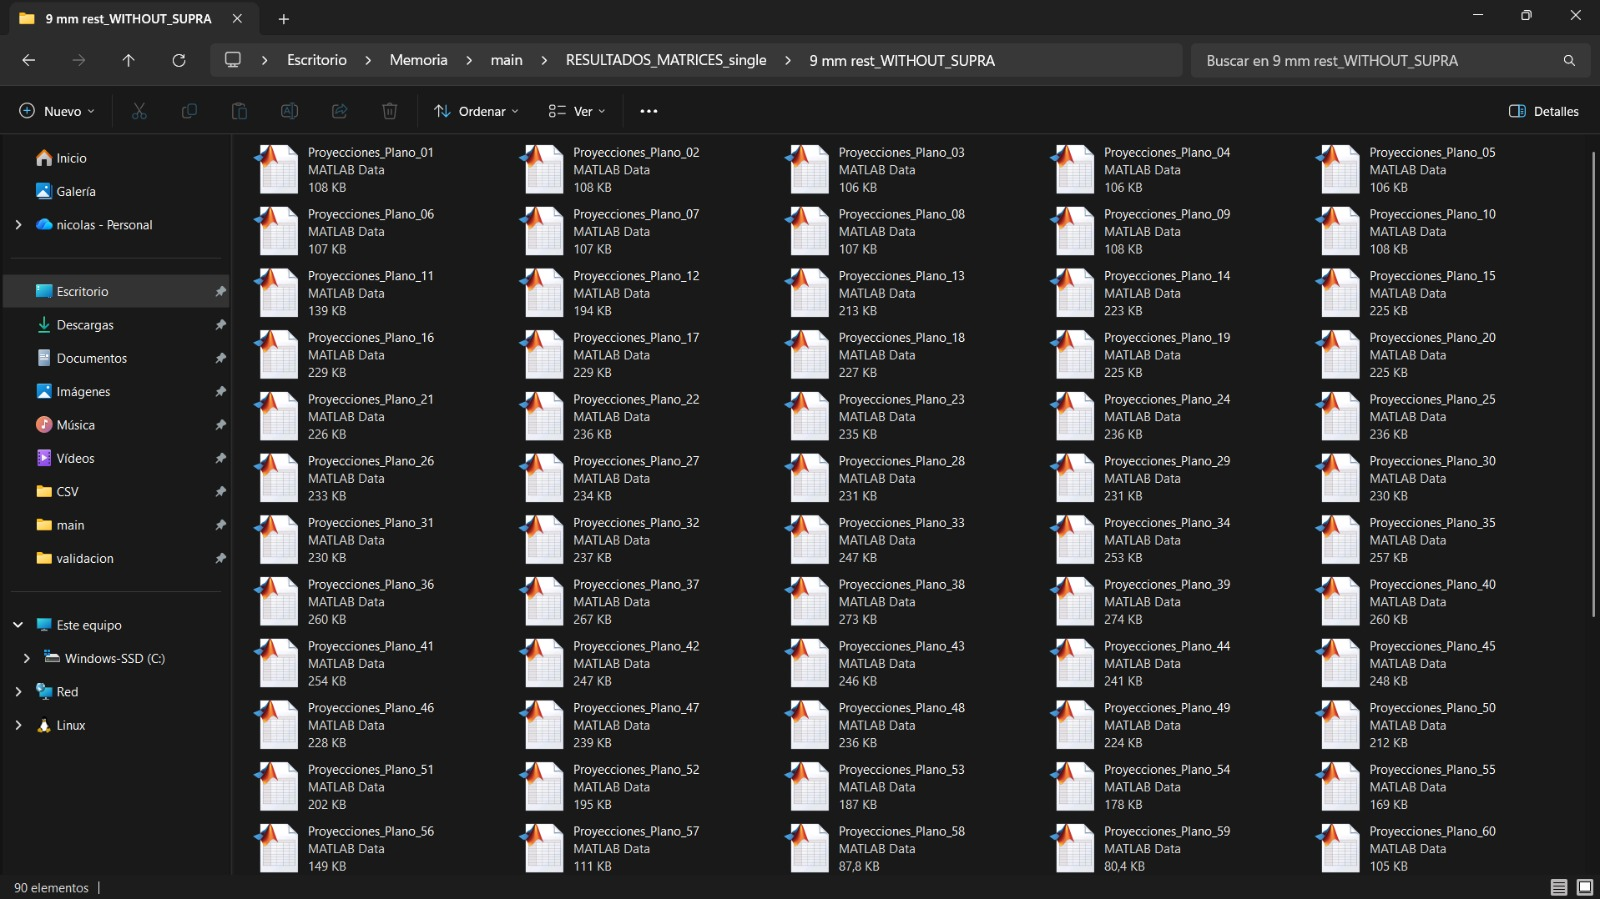
\includegraphics[width=\linewidth]{figures/validacion/fase2/carpetas_single.jpeg} 
%         \caption{Implementación preliminar: Precisión \textit{single} (32 bits)}
%         \label{fig:memoria_single}
%     \end{subfigure}
    
%     \vspace{0.4cm}
    
%     \begin{subfigure}{0.85\textwidth}
%         \centering
%         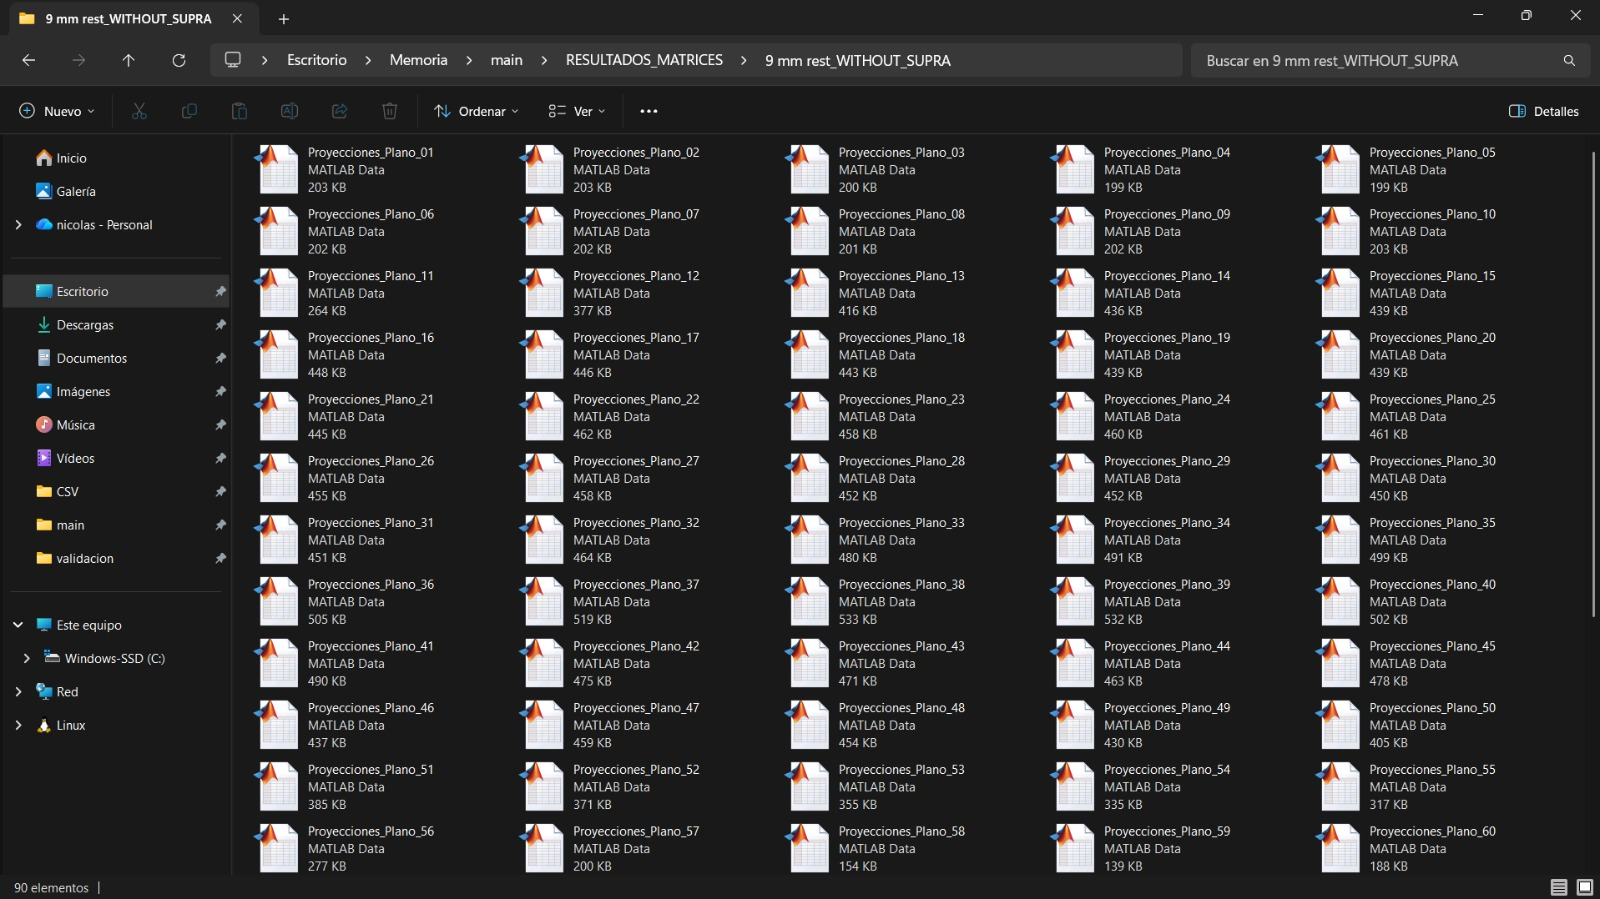
\includegraphics[width=\linewidth]{figures/validacion/fase2/carpetas_double.jpeg} 
%         \caption{Implementación definitiva: Precisión \textit{double} (64 bits)}
%         \label{fig:memoria_double}
%     \end{subfigure}
%     \caption{\label{fig:exportacion_batch_precision} Comparativa del impacto en el almacenamiento local (\textit{Storage Footprint}) generado por el orquestador. El salto hacia la alta precisión (\textit{double}) incrementó el peso por iteración de $\sim$109 KB a $\sim$204 KB; sin embargo, la exportación iterativa evitó la saturación de la RAM, garantizando la máxima integridad para la síntesis acústica. Fuente: Elaboración propia.}
% \end{figure}

% La correcta generación de este repositorio fragmentado y de alta precisión permitió que el módulo de parametrización (\textit{Feature Extraction}) iterara sobre los archivos locales de manera eficiente. El algoritmo extrajo con éxito los descriptores cinemáticos y sonoros para cada plano, culminando en la consolidación de la matriz tabular final (\textit{Dataset}). Esta estructura de datos bidimensional cierra formalmente la etapa de digitalización, sentando las bases numéricas estrictamente necesarias para la validación clínica mediante el descubrimiento de patrones no supervisados.
\newpage
\secnumbersection{CONCLUSIONES}\label{ch:conclusiones}

\subsection{Conclusiones generales}

El principal aporte de esta memoria radica en el diseño, implementación y validación de una nueva metodología computacional capaz de transformar adquisiciones hemodinámicas de \textit{4D Flow MRI} en representaciones auditivas. El desarrollo de esta nueva forma de análisis integra diferentes campos de estudio, tales como el procesamiento de imágenes médicas, el procesamiento digital de señales y la mecánica de fluidos cardiovasculares (hemodinámica).

La metodología desarrollada se materializó en dos herramientas computacionales principales:

\begin{itemize}
    \item \textbf{Explorador hemodinámico:} Constituyó el núcleo del motor acústico y espectral. Operó como la plataforma base durante las fases iniciales para iterar sobre los algoritmos de proyección de velocidades y definir las estrategias de síntesis sonora.

    \item \textbf{Comparador interactivo:} Se consolidó como el instrumento principal para la evaluación cruzada de los escenarios de estudio. Heredando la arquitectura de procesamiento del \textit{Explorador hemodinámico}, esta interfaz facilitó un contraste rápido, simultáneo y eficiente de las firmas acústicas y espectrales entre las distintas morfologías.
\end{itemize}

A través de la utilización de estas interfaces sobre los datos extraídos de los diferentes fantomas, se logró evaluar empíricamente el desempeño del modelo computacional. Los resultados evidencian la capacidad de este último para producir salidas concordantes con la entrada hemodinámica local. De esta manera, se demuestra la aptitud del sistema para capturar y traducir las variaciones del fluido en firmas acústicas y espectrales distintivas.

Se comprobó que el mapeo sonoro es sensible a la física del sistema. Al evaluar los distintos grados de coartación bajo condiciones de estrés, las representaciones espectrales mostraron cambios proporcionales a su nivel. Así, se confirma que la sonificación resultante actúa como un reflejo del comportamiento del fluido.


Adicionalmente, el análisis estadístico y de aprendizaje no supervisado permitió capturar el valor analítico de los descriptores extraídos. Mediante el Análisis de Componentes Principales (\textit{PCA}), se comprobó que las características espectrales —particularmente los coeficientes cepstrales (\textit{MFCCs})— poseen un peso estadístico equivalente a las variables cinemáticas dentro de un modelo multimodal. Sin embargo, la evaluación del agrupamiento autónomo mediante \textit{K-Means} reveló que, si bien el dominio cinemático presenta una alta separabilidad geométrica, la incorporación de las características acústicas introduce una mayor complejidad topológica, resultando en agrupamientos más débiles. En conclusión, aunque bajo los criterios de sonificación establecidos el sonido sintetizado es un descriptor paramétricamente robusto para capturar la varianza del flujo, su naturaleza requiere enfoques distintos para tareas de clasificación.

\subsection{Cumplimiento de objetivos}

El objetivo general de esta memoria se alcanzó de manera satisfactoria mediante el cumplimiento progresivo de los objetivos específicos planteados:

En primer lugar, la extracción y procesamiento de métricas cinemáticas se logró con éxito mediante la asimilación de las matrices volumétricas de \textit{4D Flow MRI}. El algoritmo implementado permitió discretizar el dominio espacial a lo largo del \textit{centerline}, extrayendo perfiles transversales que facilitaron el cálculo de variables como la velocidad máxima, la varianza espacial y el índice de pulsatilidad.

En segundo lugar, la síntesis de características acústicas se concretó a través del desarrollo del motor de sonificación. Este módulo logró emular computacionalmente el ultrasonido Doppler, mapeando directamente los parámetros hemodinámicos locales hacia señales de audio. De estas señales se extrajeron descriptores como los coeficientes cepstrales de Mel (\textit{MFCCs}).

El tercer objetivo se materializó con la programación de las herramientas de análisis, destacando el \textit{Explorador hemodinámico} y el \textit{Comparador interactivo}. Estas interfaces gráficas permitieron la navegación espacial sobre la geometría tridimensional del vaso sanguíneo, logrando una sincronización precisa entre la posición anatómica, la retroalimentación visual (espectrogramas) y la reproducción auditiva.

Finalmente, la coherencia del espacio de características fue validada empíricamente al contrastar como los distintos fantomas bajo condiciones de reposo y estrés producen firmas acústicas distinguibles entre sí. De este modo, se confirma que el modelo de sonificación logra una traducción fiel, donde la severidad de la coartación y el estrés del caudal generan firmas sonoras coherentes y perceptualmente distinguibles.

\subsection{Trabajo a futuro}

A partir de los resultados obtenidos y las limitaciones identificadas durante el desarrollo de esta memoria, se proponen las siguientes líneas de investigación para la expansión y optimización de la metodología:

\begin{itemize}
    \item \textbf{Optimización de la emulación Doppler:} Aunque el motor actual considera el ángulo de insonación y el volumen de muestra, su implementación inicial asume condiciones idealizadas. Se propone desarrollar un modelo de insonación dinámico, donde el ángulo de incidencia y las dimensiones del volumen de muestra sean espacialmente variables.

    \item \textbf{Exploración de estrategias de sonificación:} Dado que el esquema de parametrización actual en \textit{PMSon} se basó en criterios heurísticos y experiencia en síntesis de audio, existe un amplio margen para investigar nuevas formas de representación. Se sugiere diseñar y evaluar nuevas lógicas de mapeo de  parámetros, posiblemente integrando estudios psicoacústicos que determinen qué timbres o motores de síntesis facilitan una mejor discriminación auditiva para el usuario.
    
    \item \textbf{Expansión del análisis no supervisado:} Se propone ampliar el espacio de características acústicas extraídas para enriquecer la representación matemática. Asimismo, para superar los agrupamientos débiles observados, se plantea sustituir o complementar \textit{K-Means} con otros algoritmos de aprendizaje no supervisado capaces de manejar topologías de datos más complejas.
    
    \item \textbf{Validación clínica (\textit{in-vivo}):} El paso fundamental para consolidar esta herramienta es su transición hacia el procesamiento de adquisiciones \textit{4D Flow MRI} reales. Evaluar el sistema con datos \textit{in-vivo} permitirá medir la robustez del algoritmo frente a variaciones biológicas.
\end{itemize}

\newpage
\secnumberlesssection{ANEXOS}

\section{Matrices de contingencia del agrupamiento K-Means}
\label{anexo:matrices_kmeans}

Se presentan las tablas de contingencia que detallan la distribución cuantitativa de cada clúster descubierto por el algoritmo \textit{K-Means} ($k=4$). 
\begin{table}[H]
\centering
\caption{Tabla de contingencia: Distribución de planos anatómicos por clúster para el dominio de características cinemáticas.}
\label{tab:anexo_cinematico}
\resizebox{\textwidth}{!}{
\begin{tabular}{lcccccccc}
\hline
 & \multicolumn{2}{c}{\textbf{Fantoma Normal}} & \multicolumn{2}{c}{\textbf{Estenosis 9 mm}} & \multicolumn{2}{c}{\textbf{Estenosis 11 mm}} & \multicolumn{2}{c}{\textbf{Estenosis 13 mm}} \\ \cline{2-9} 
\textbf{Clúster asignado} & \textit{Rest} & \textit{Stress} & \textit{Rest} & \textit{Stress} & \textit{Rest} & \textit{Stress} & \textit{Rest} & \textit{Stress} \\ \hline
\textbf{Clúster 1} & 12 & 16 & 19 & 16 & 28 & 29 & 30 & 36 \\
\textbf{Clúster 2} & 0 & 0 & 20 & 26 & 8 & 11 & 0 & 0 \\
\textbf{Clúster 3} & 67 & 63 & 39 & 34 & 42 & 36 & 48 & 40 \\
\textbf{Clúster 4} & 11 & 11 & 12 & 14 & 12 & 14 & 12 & 14 \\ \hline
\end{tabular}
}
\end{table}

\begin{table}[H]
\centering
\caption{Tabla de contingencia: Distribución de planos anatómicos por clúster para el dominio de características acústicas.}
\label{tab:anexo_acustico}
\resizebox{\textwidth}{!}{
\begin{tabular}{lcccccccc}
\hline
 & \multicolumn{2}{c}{\textbf{Fantoma Normal}} & \multicolumn{2}{c}{\textbf{Estenosis 9 mm}} & \multicolumn{2}{c}{\textbf{Estenosis 11 mm}} & \multicolumn{2}{c}{\textbf{Estenosis 13 mm}} \\ \cline{2-9} 
\textbf{Clúster asignado} & \textit{Rest} & \textit{Stress} & \textit{Rest} & \textit{Stress} & \textit{Rest} & \textit{Stress} & \textit{Rest} & \textit{Stress} \\ \hline
\textbf{Clúster 1} & 48 & 22 & 24 & 10 & 28 & 11 & 30 & 12 \\
\textbf{Clúster 2} & 4 & 7 & 17 & 24 & 10 & 14 & 8 & 15 \\
\textbf{Clúster 3} & 0 & 45 & 9 & 47 & 4 & 58 & 3 & 52 \\
\textbf{Clúster 4} & 38 & 16 & 40 & 9 & 48 & 7 & 49 & 11 \\ \hline
\end{tabular}
}
\end{table}

\begin{table}[H]
\centering
\caption{Tabla de contingencia: Distribución de planos anatómicos por clúster para el dominio multimodal.}
\label{tab:anexo_multimodal}
\resizebox{\textwidth}{!}{
\begin{tabular}{lcccccccc}
\hline
 & \multicolumn{2}{c}{\textbf{Fantoma Normal}} & \multicolumn{2}{c}{\textbf{Estenosis 9 mm}} & \multicolumn{2}{c}{\textbf{Estenosis 11 mm}} & \multicolumn{2}{c}{\textbf{Estenosis 13 mm}} \\ \cline{2-9} 
\textbf{Clúster asignado} & \textit{Rest} & \textit{Stress} & \textit{Rest} & \textit{Stress} & \textit{Rest} & \textit{Stress} & \textit{Rest} & \textit{Stress} \\ \hline
\textbf{Clúster 1} & 14 & 49 & 29 & 30 & 31 & 37 & 31 & 47 \\
\textbf{Clúster 2} & 3 & 6 & 23 & 36 & 16 & 28 & 7 & 16 \\
\textbf{Clúster 3} & 11 & 11 & 12 & 13 & 13 & 13 & 14 & 14 \\
\textbf{Clúster 4} & 62 & 24 & 26 & 11 & 30 & 12 & 38 & 13 \\ \hline
\end{tabular}
}
\end{table}

\section{Exploración perceptiva y espectral bajo condición de reposo (\textit{rest})}
\label{anexo:comparacion_casos}
En este anexo se documenta la evolución espectral y acústica de los cuatro modelos morfológicos (Normal, 13 mm, 11 mm y 9 mm) evaluados bajo la condición hemodinámica de reposo (\textit{rest}). Se mantiene la misma discretización espacial definida en el análisis principal para facilitar la comparación cruzada.

\subsection{Análisis comparativo: Aorta ascendente (plano 21)}

\begin{figure}[H]
    \centering
    \begin{minipage}{0.75\textwidth}
        \begin{subfigure}{0.48\linewidth}
            \centering
            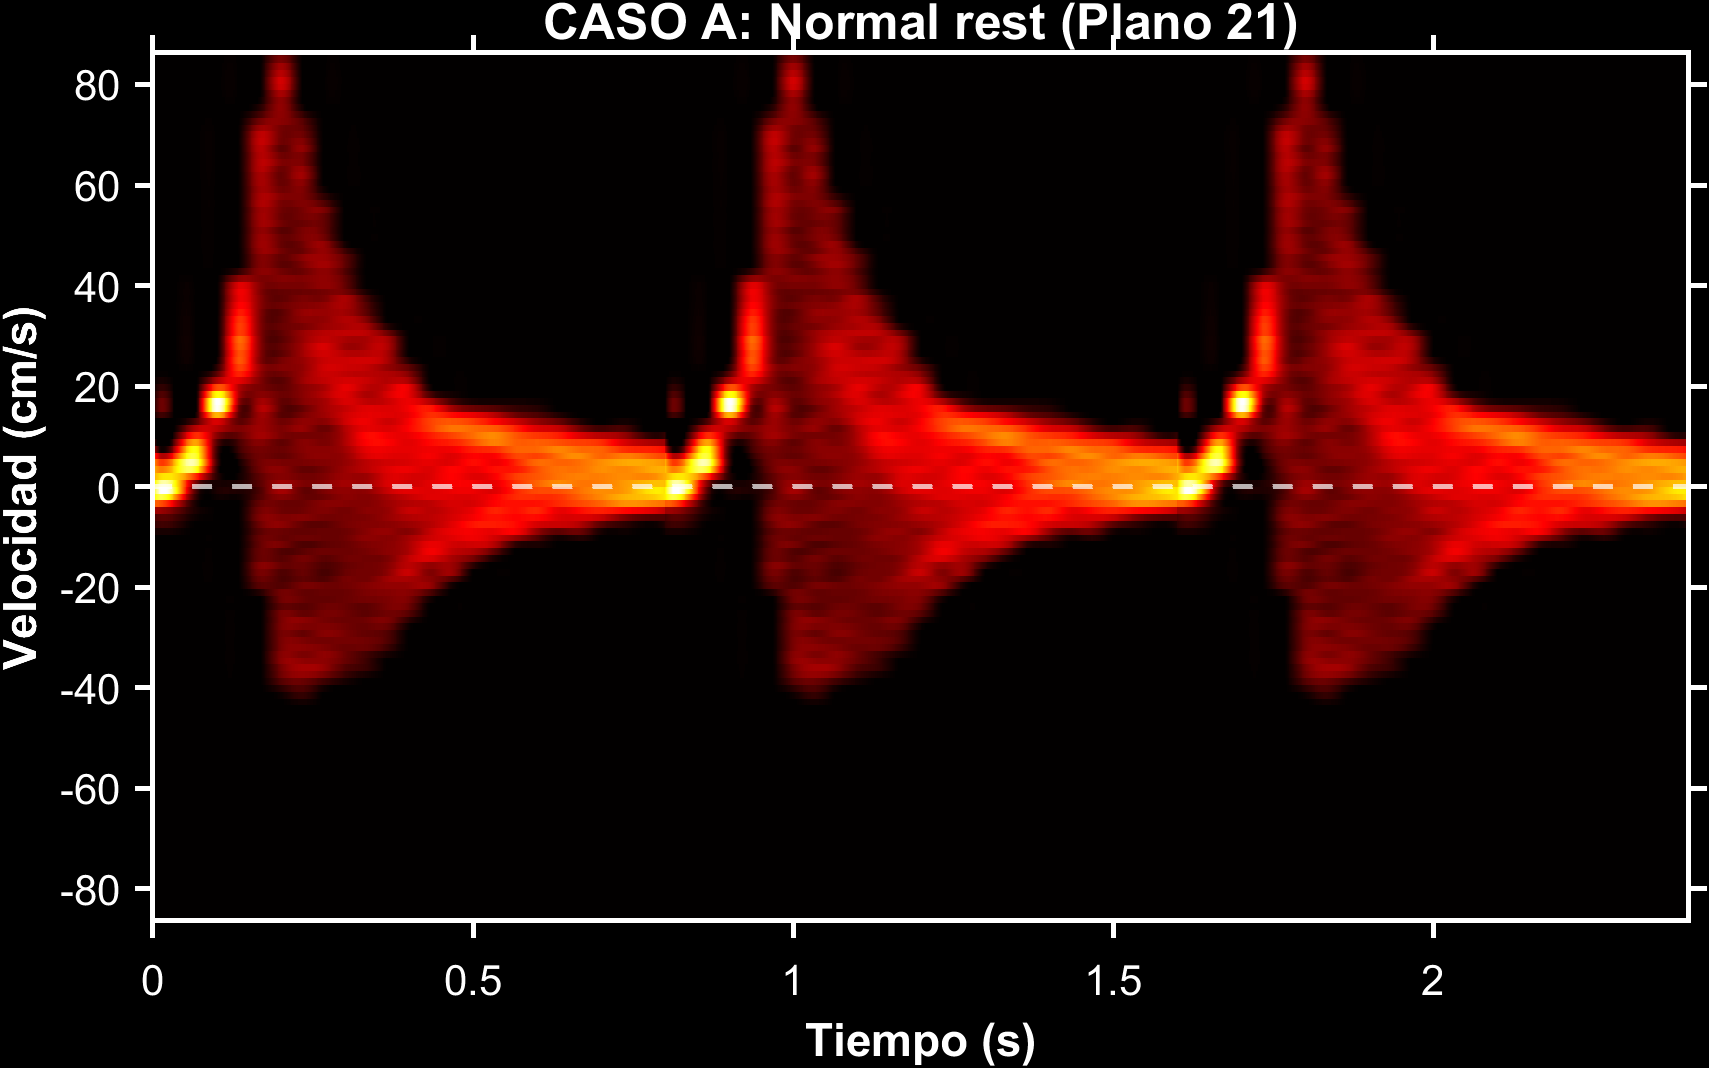
\includegraphics[width=\linewidth]{figures/anexos/Normal_rest_Plano21.png}
            \caption{\href{https://drive.google.com/file/d/1ZKAqWONgGDq1fNld8xxtLIQJTtJ9YBZD/view?usp=sharing}{Fantoma normal \textbf{(Escuchar)}}}
            \label{fig:anexo_p21_normal}
        \end{subfigure}\hfill
        \begin{subfigure}{0.48\linewidth}
            \centering
            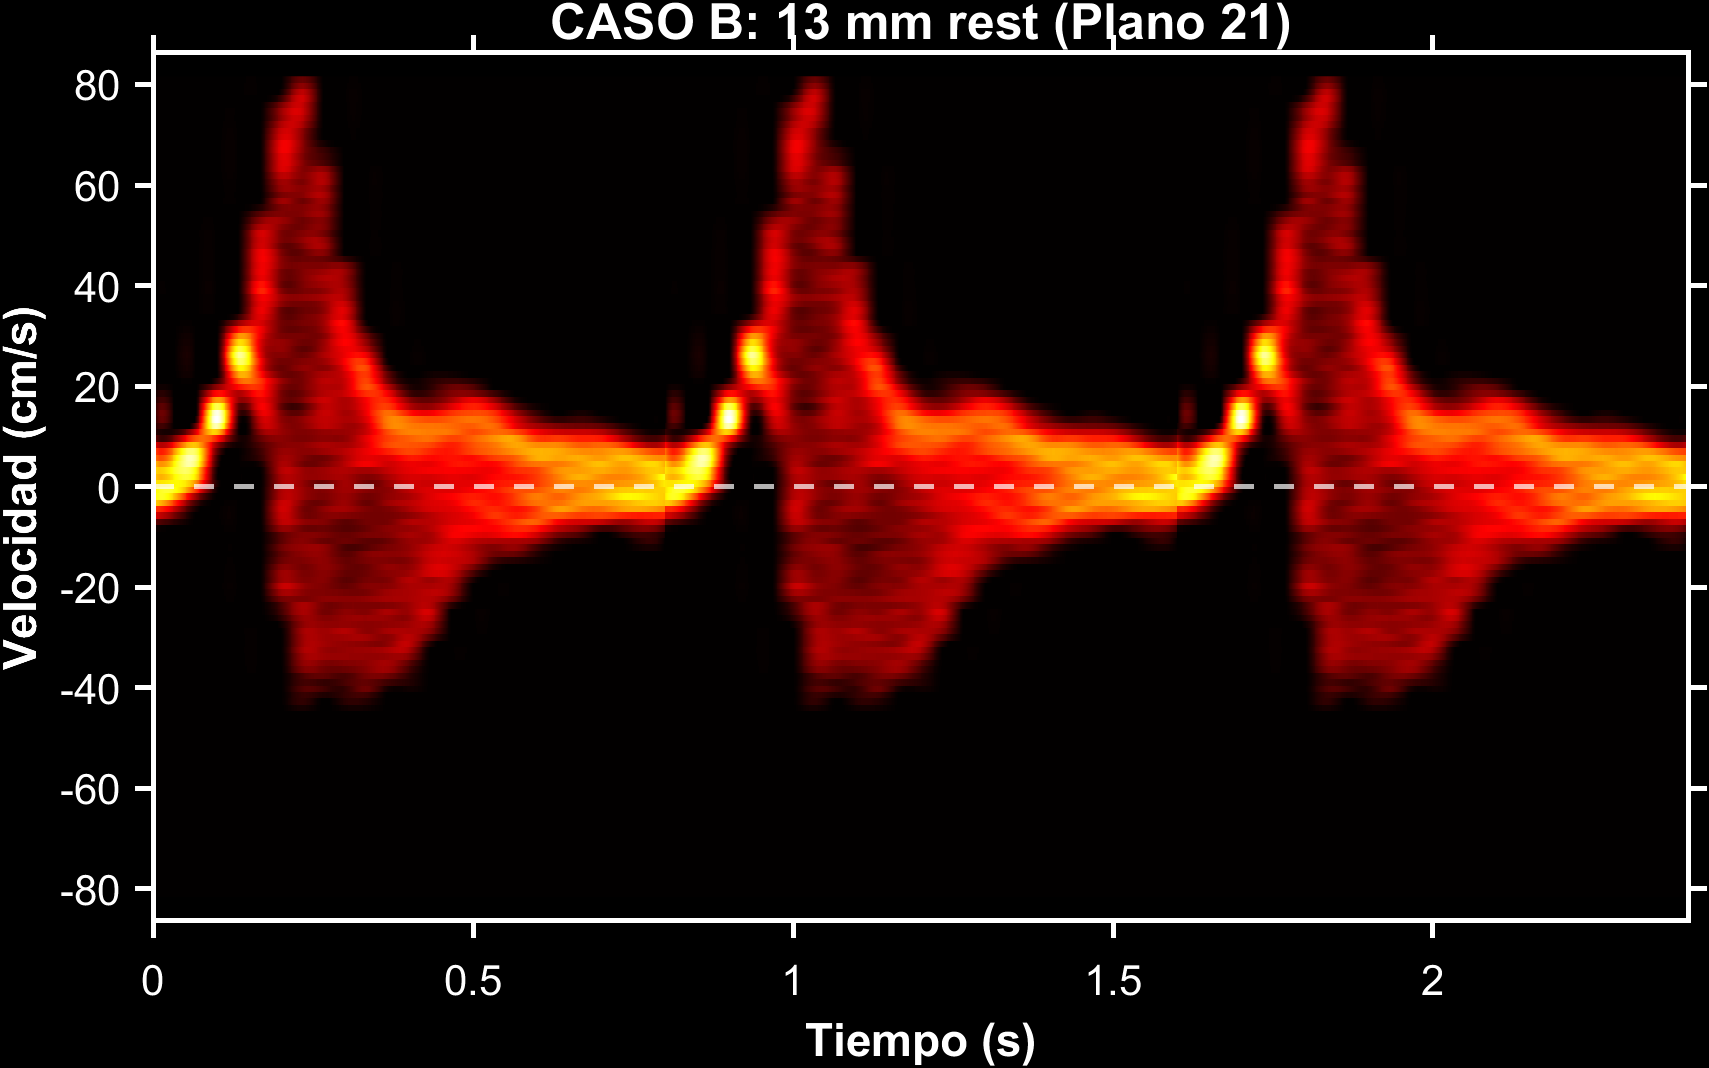
\includegraphics[width=\linewidth]{figures/anexos/13_mm_rest_Plano21.png}
            \caption{\href{https://drive.google.com/file/d/1NNRotryh_QmV-Zc-VIlffoJ7tDrSEmsP/view?usp=sharing}{Fantoma 13 mm \textbf{(Escuchar)}}}
            \label{fig:anexo_p21_13mm}
        \end{subfigure}
        
        \vspace{0.4cm}
        
        \begin{subfigure}{0.48\linewidth}
            \centering
            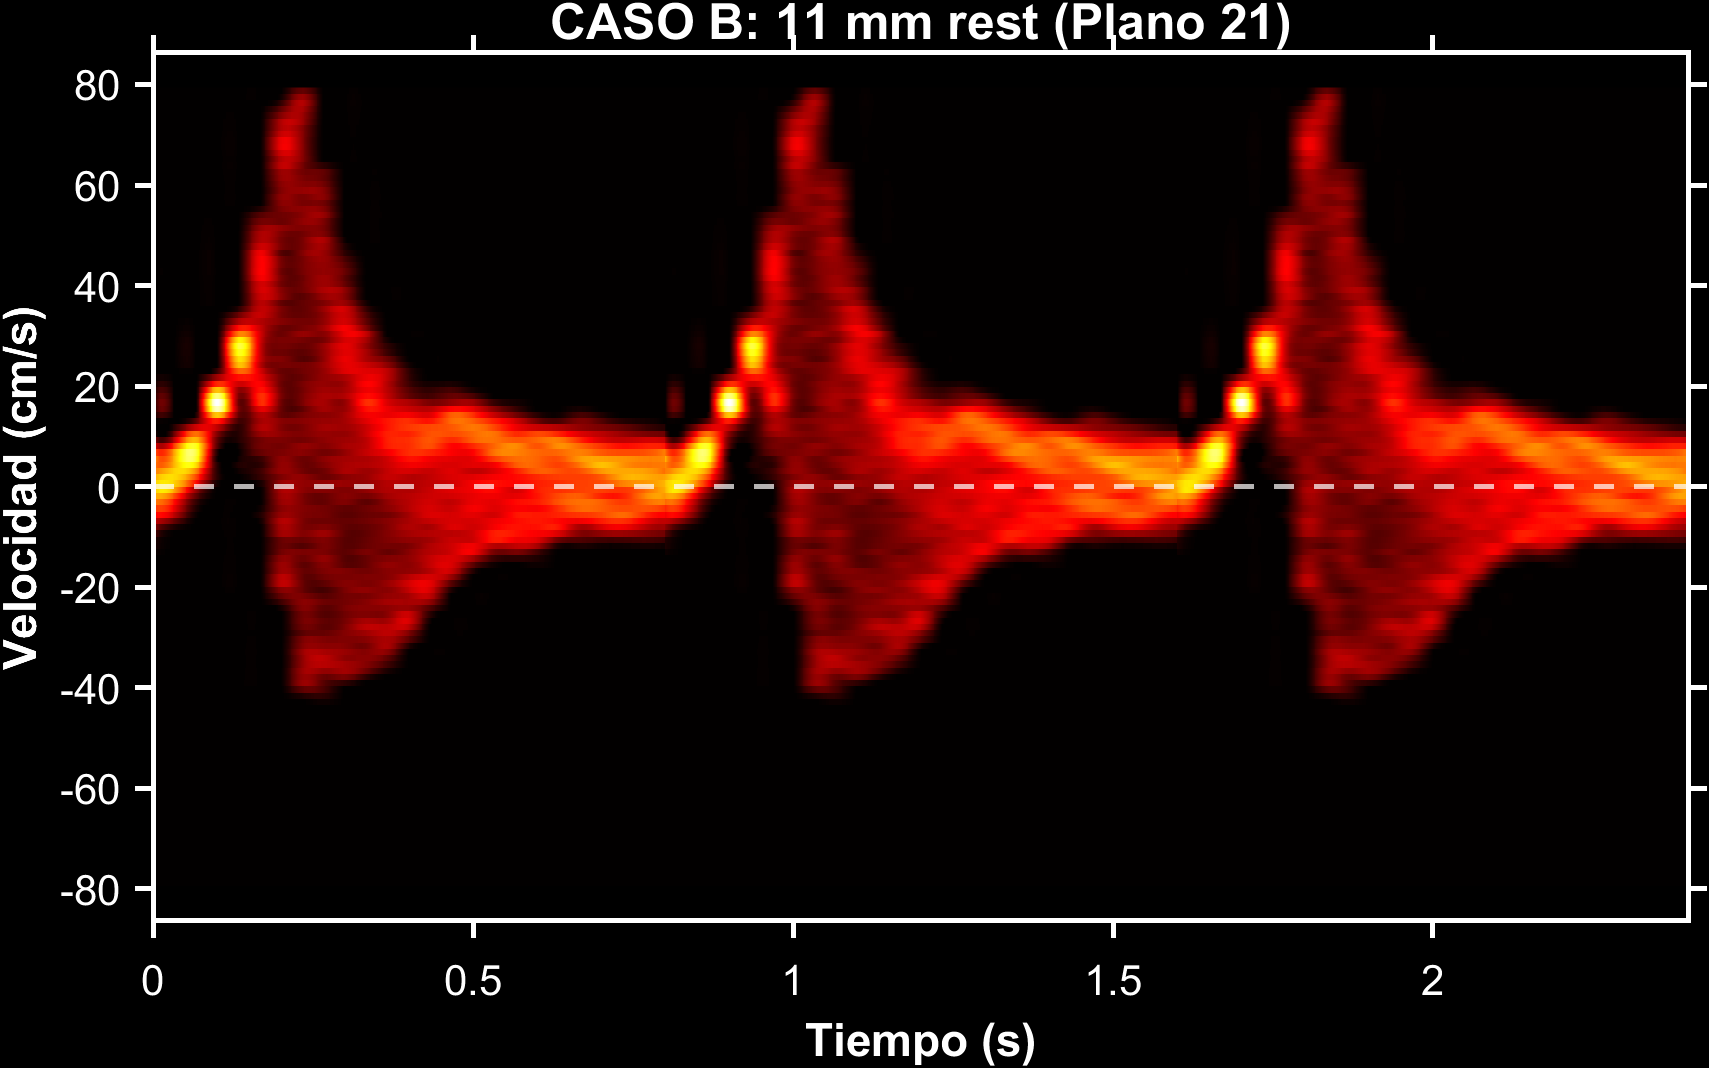
\includegraphics[width=\linewidth]{figures/anexos/11_mm_rest_Plano21.png}
            \caption{\href{https://drive.google.com/file/d/1eQq_XtXl69I2DC_eBFoO1hlGUNPU-k-t/view?usp=sharing}{Fantoma 11 mm \textbf{(Escuchar)}}}
            \label{fig:anexo_p21_11mm}
        \end{subfigure}\hfill
        \begin{subfigure}{0.48\linewidth}
            \centering
            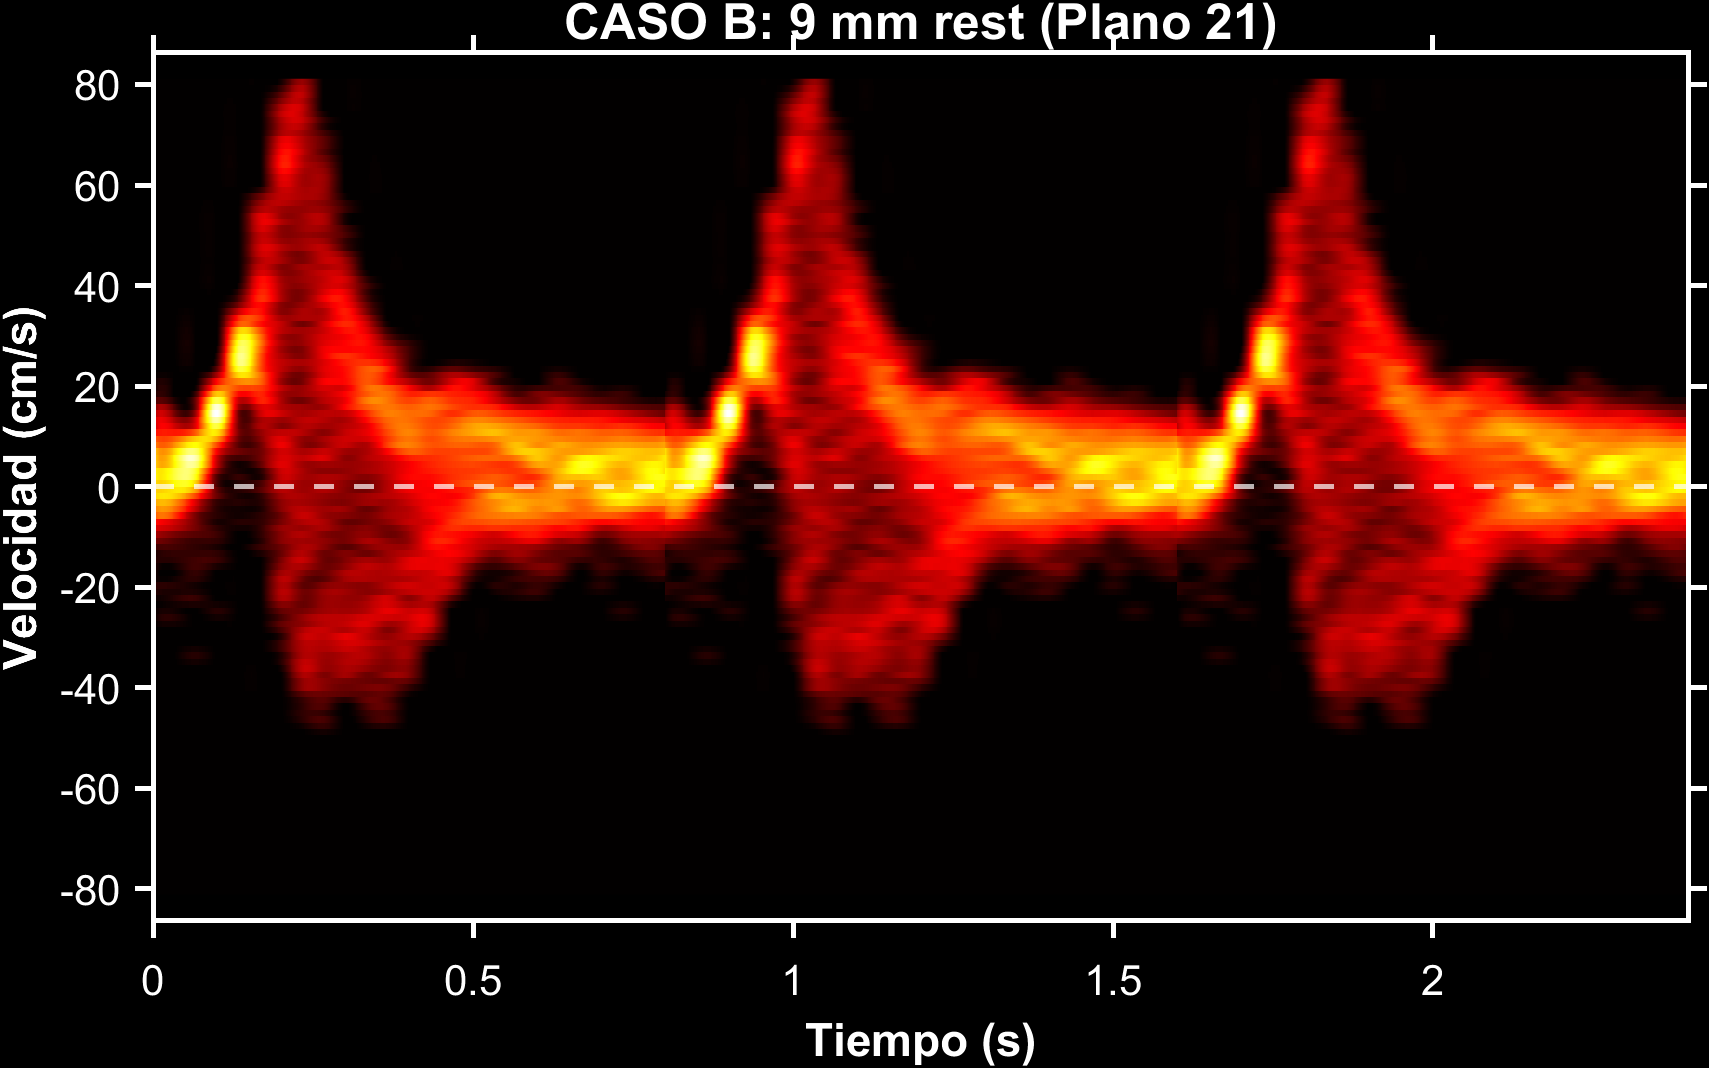
\includegraphics[width=\linewidth]{figures/anexos/9_mm_rest_Plano21.png}
            \caption{\href{https://drive.google.com/file/d/1aXkjKpO1hv90QrdGfdTchuTl22igPRqt/view?usp=sharing}{Fantoma 9 mm \textbf{(Escuchar)}}}
            \label{fig:anexo_p21_9mm}
        \end{subfigure}
    \end{minipage}
    \caption{\label{fig:anexo_comparacion_p21} Evolución espectral en la zona de la aorta ascendente bajo condición de reposo. Fuente: Elaboración propia.}
\end{figure}


\subsection{Análisis comparativo: Arco aórtico (plano 45)}

\begin{figure}[H]
    \centering
    \begin{minipage}{0.75\textwidth}
        \begin{subfigure}{0.48\linewidth}
            \centering
            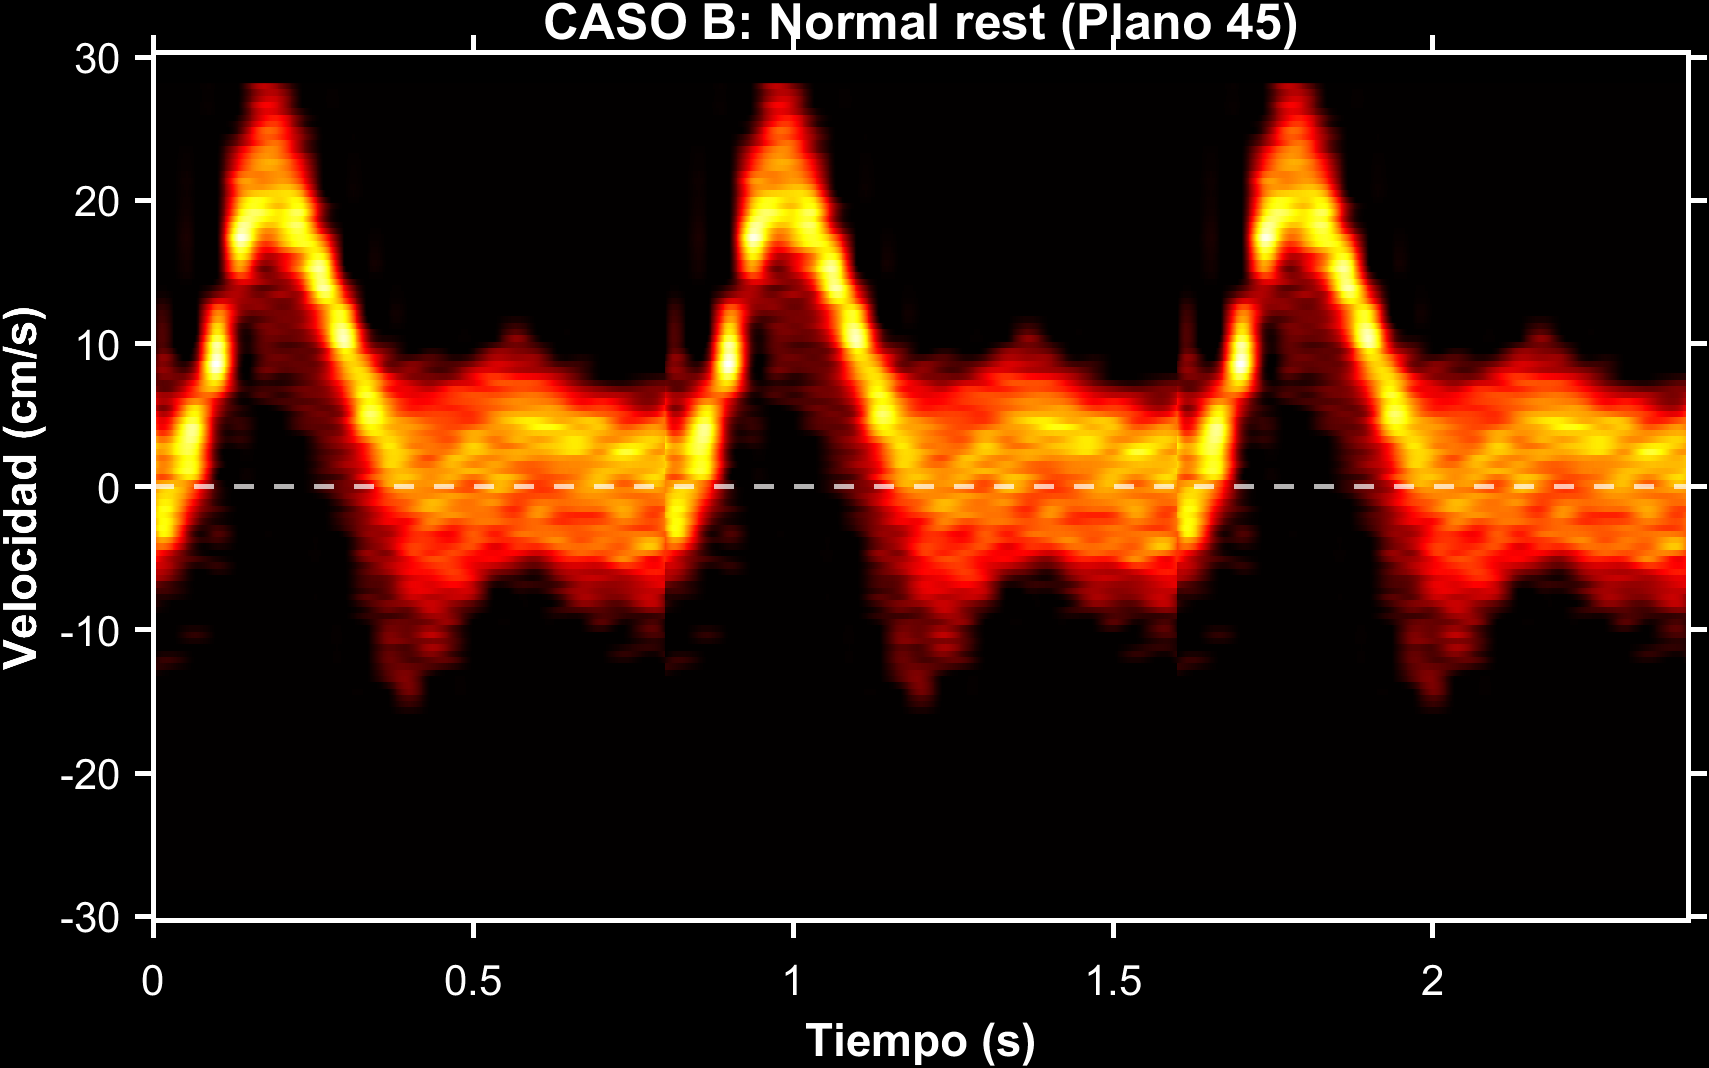
\includegraphics[width=\linewidth]{figures/anexos/Normal_rest_Plano45.png}
            \caption{\href{https://drive.google.com/file/d/1bsp7yoFzJn6wdYWwkefdBuo5repDJPdR/view?usp=sharing}{Fantoma normal \textbf{(Escuchar)}}}
            \label{fig:anexo_p45_normal}
        \end{subfigure}\hfill
        \begin{subfigure}{0.48\linewidth}
            \centering
            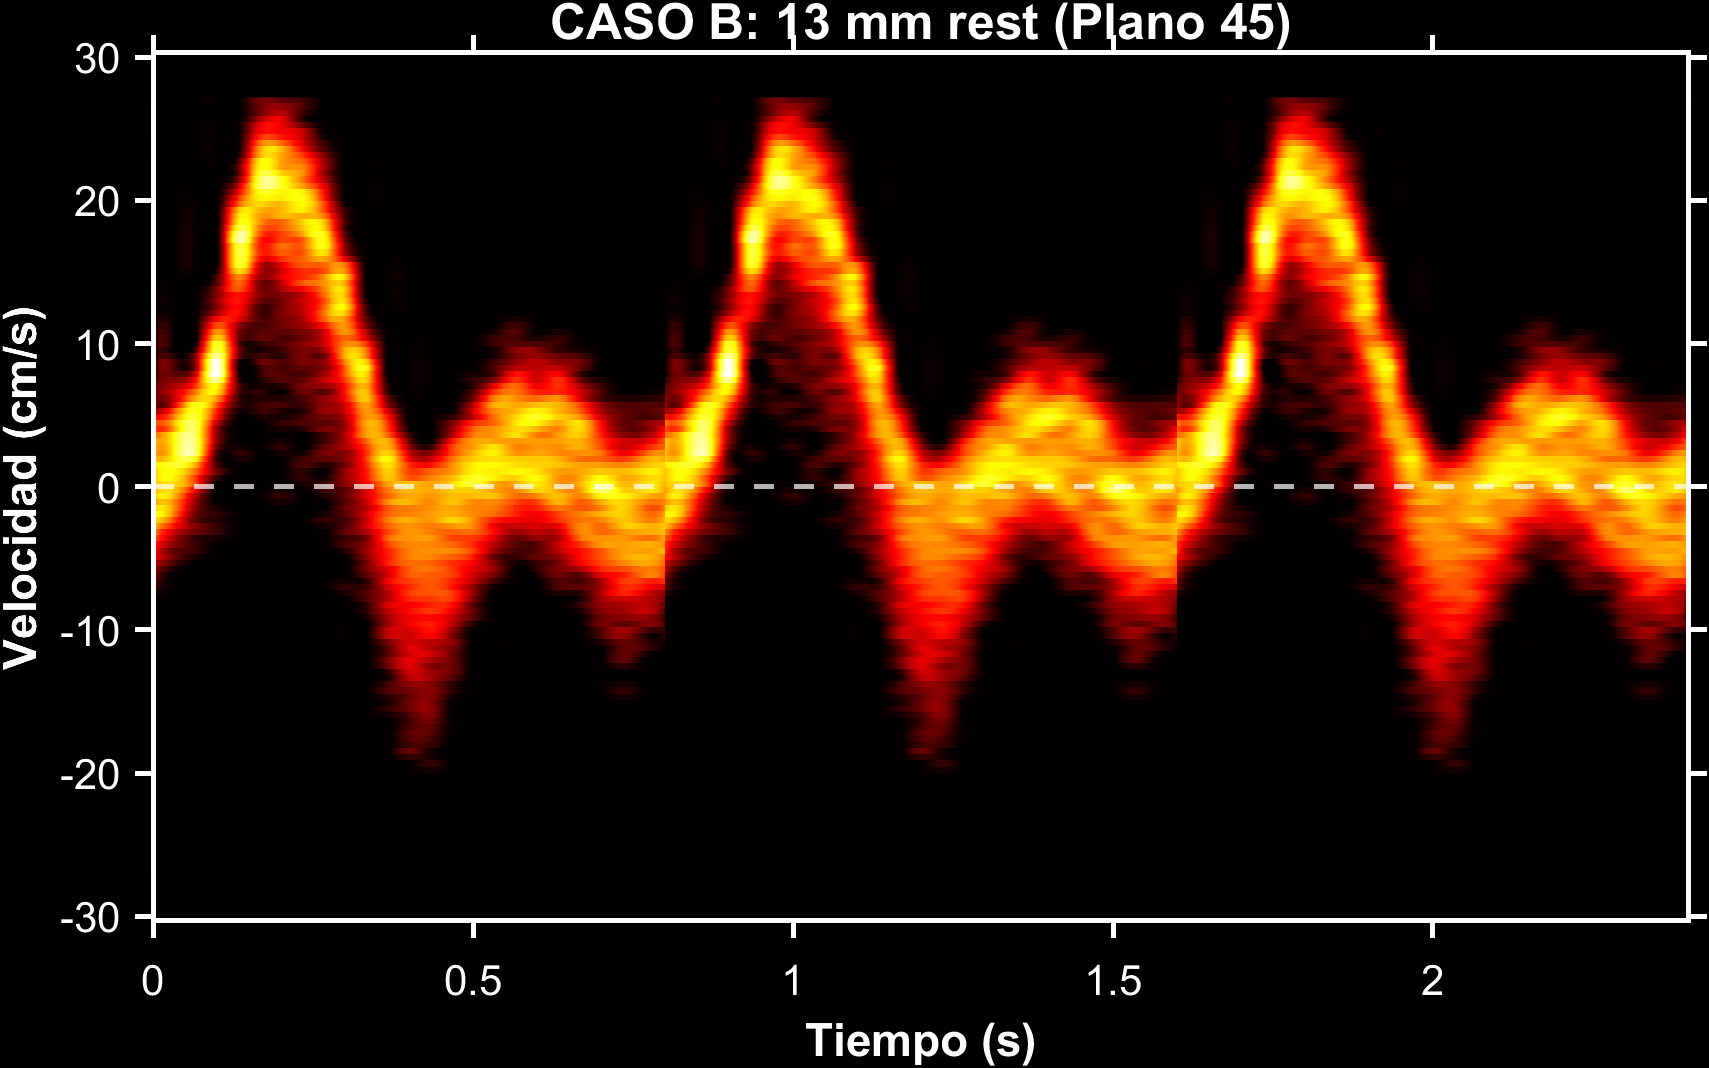
\includegraphics[width=\linewidth]{figures/anexos/13_mm_rest_Plano45.png}
            \caption{\href{https://drive.google.com/file/d/1LgYvr6ug48dCXbW_NYl_JJqlRzGxxMOV/view?usp=sharing}{Fantoma 13 mm \textbf{(Escuchar)}}}
            \label{fig:anexo_p45_13mm}
        \end{subfigure}
        
        \vspace{0.4cm}
        
        \begin{subfigure}{0.48\linewidth}
            \centering
            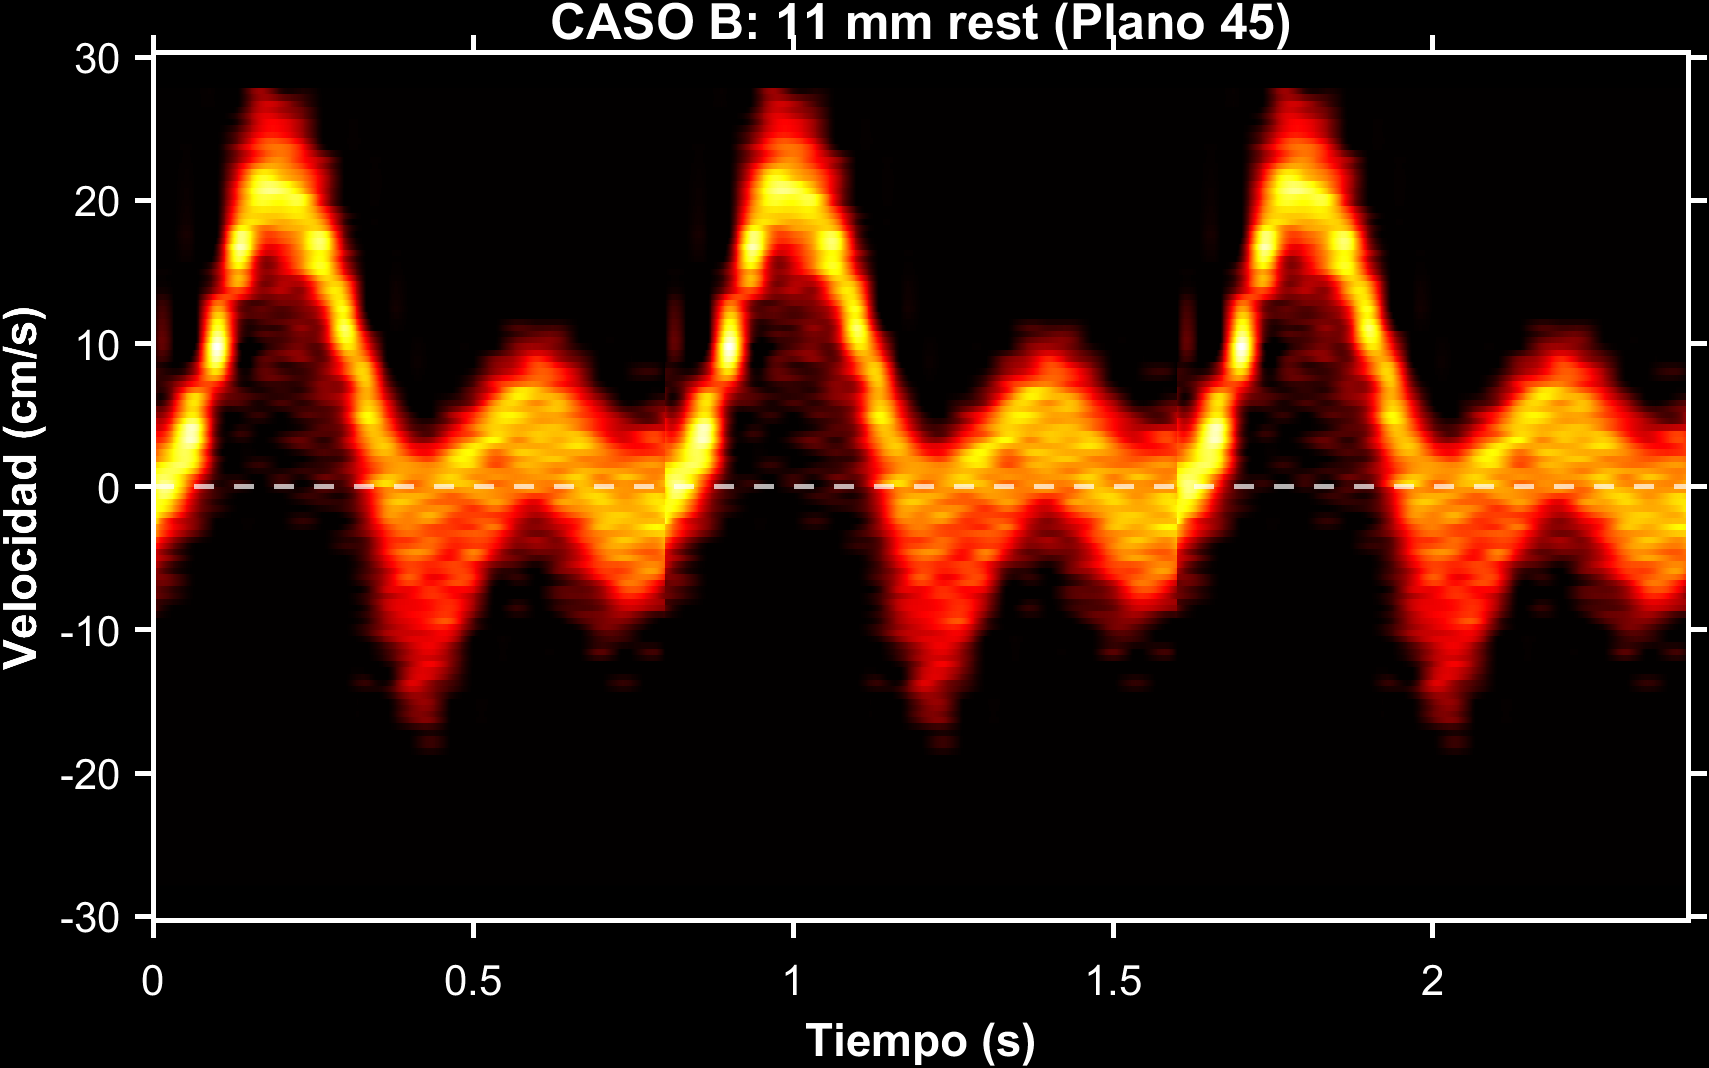
\includegraphics[width=\linewidth]{figures/anexos/11_mm_rest_Plano45.png}
            \caption{\href{https://drive.google.com/file/d/13VOYyAe2TLGDEpzZFB-JEHpD3smXe__b/view?usp=sharing}{Fantoma 11 mm \textbf{(Escuchar)}}}
            \label{fig:anexo_p45_11mm}
        \end{subfigure}\hfill
        \begin{subfigure}{0.48\linewidth}
            \centering
            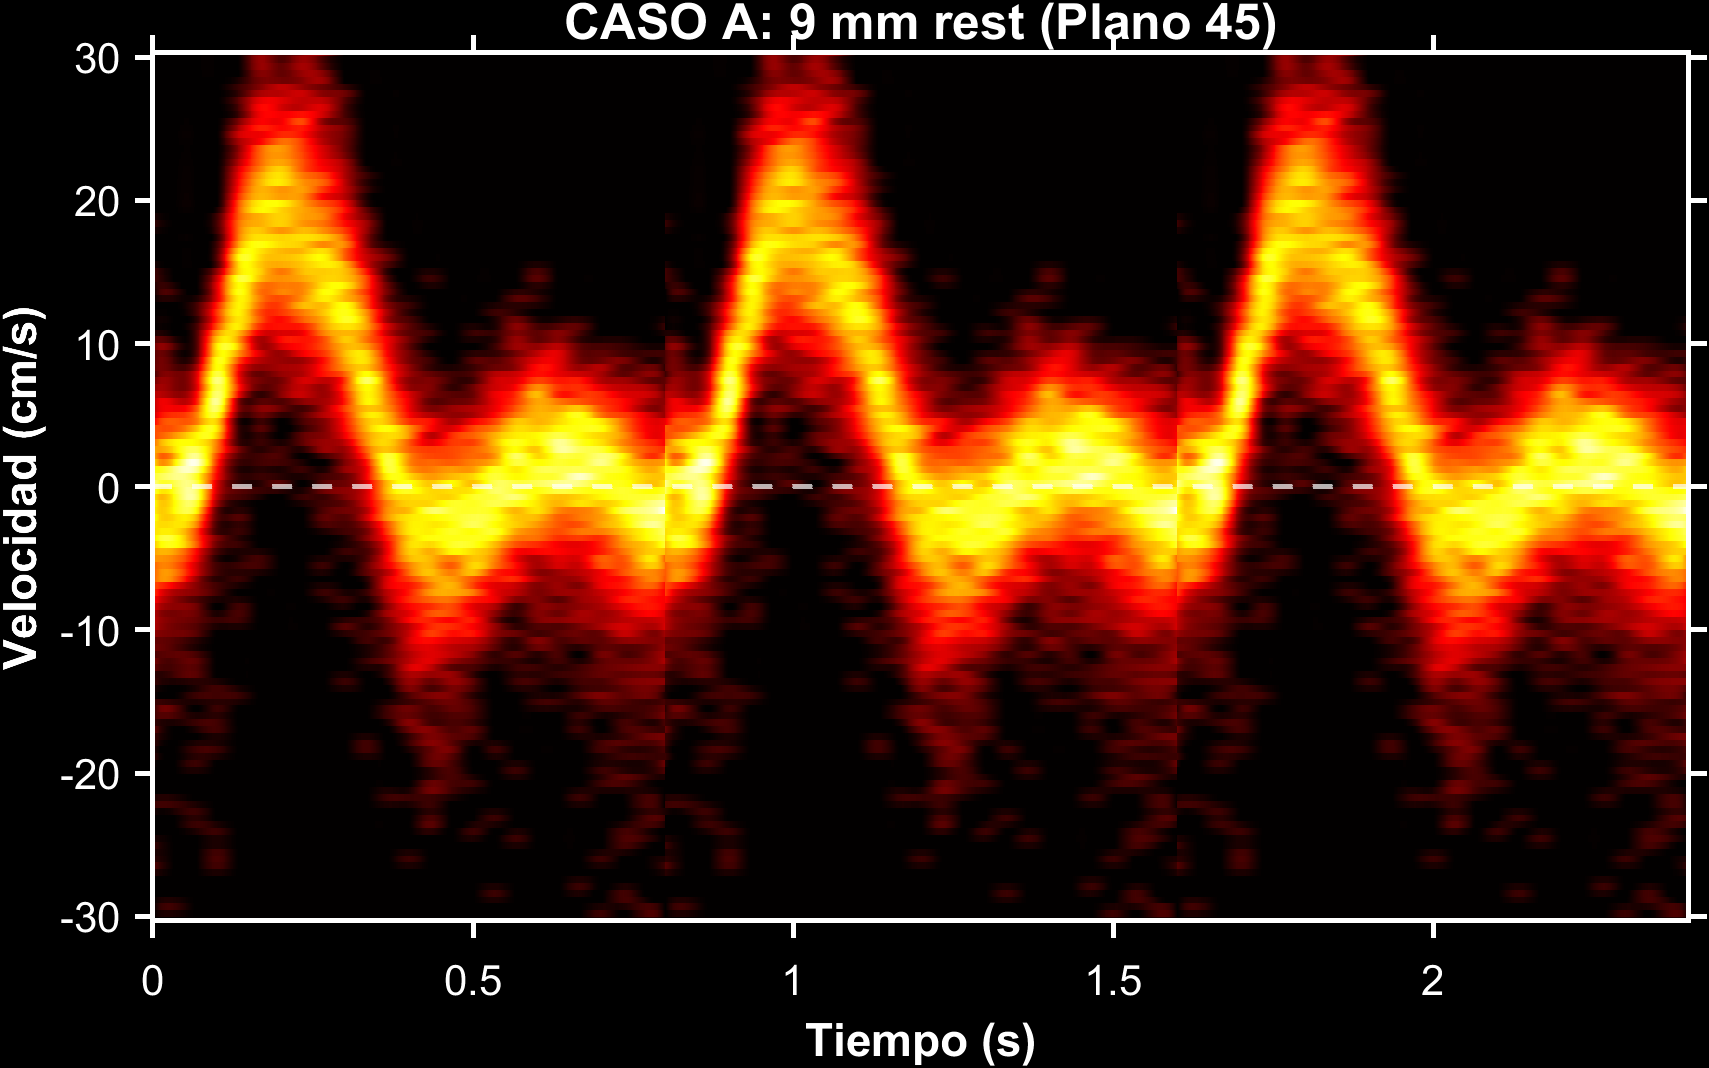
\includegraphics[width=\linewidth]{figures/anexos/9_mm_rest_Plano45.png}
            \caption{\href{https://drive.google.com/file/d/1a5bmth4i0mA5p9IGHgH1vpA63KkmTlW6/view?usp=sharing}{Fantoma 9 mm \textbf{(Escuchar)}}}
            \label{fig:anexo_p45_9mm}
        \end{subfigure}
    \end{minipage}
    \caption{\label{fig:anexo_comparacion_p45}Evolución espectral en la zona del arco aórtico bajo condición de reposo. Fuente: Elaboración propia.}
\end{figure}


\subsection{Análisis comparativo: Pre-coartación (plano 53)}

\begin{figure}[H]
    \centering
    \begin{minipage}{0.75\textwidth}
        \begin{subfigure}{0.48\linewidth}
            \centering
            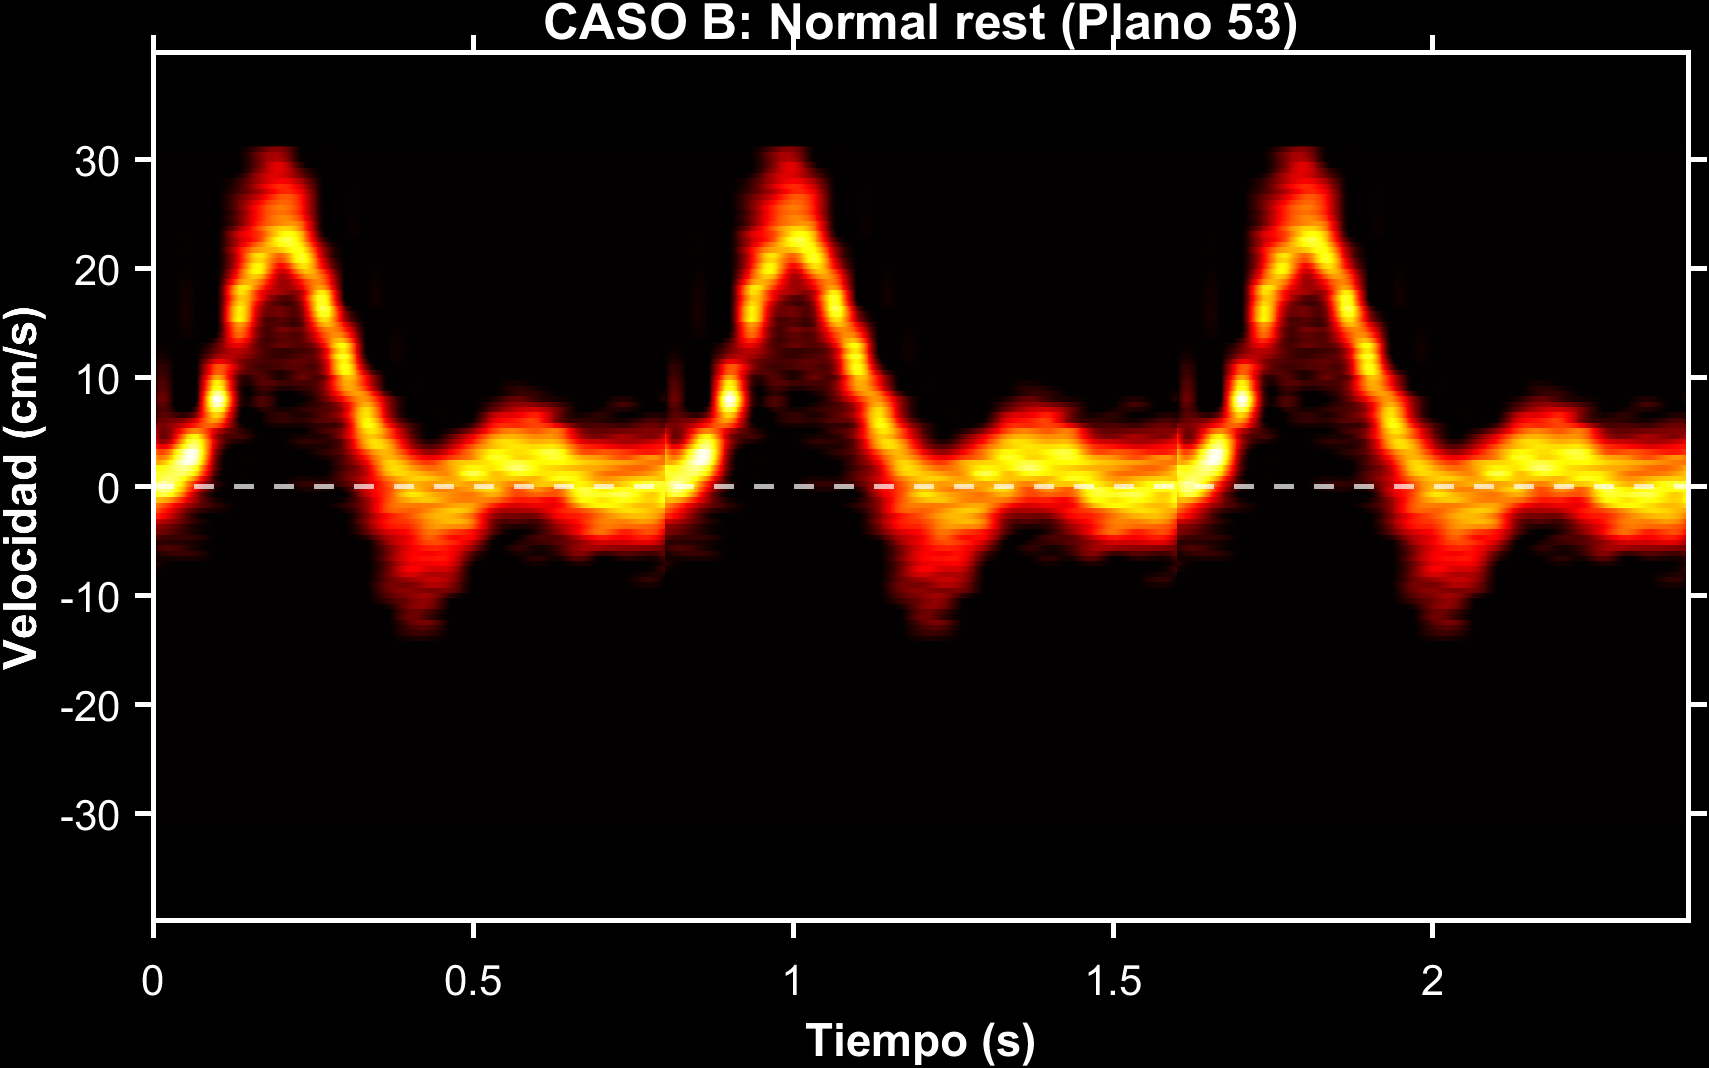
\includegraphics[width=\linewidth]{figures/anexos/Normal_rest_Plano53.png}
            \caption{\href{https://drive.google.com/file/d/1HOFjscXZdn0Xqr6QBVaSOorMYazGTOI1/view?usp=sharing}{Fantoma normal \textbf{(Escuchar)}}}
            \label{fig:anexo_p53_normal}
        \end{subfigure}\hfill
        \begin{subfigure}{0.48\linewidth}
            \centering
            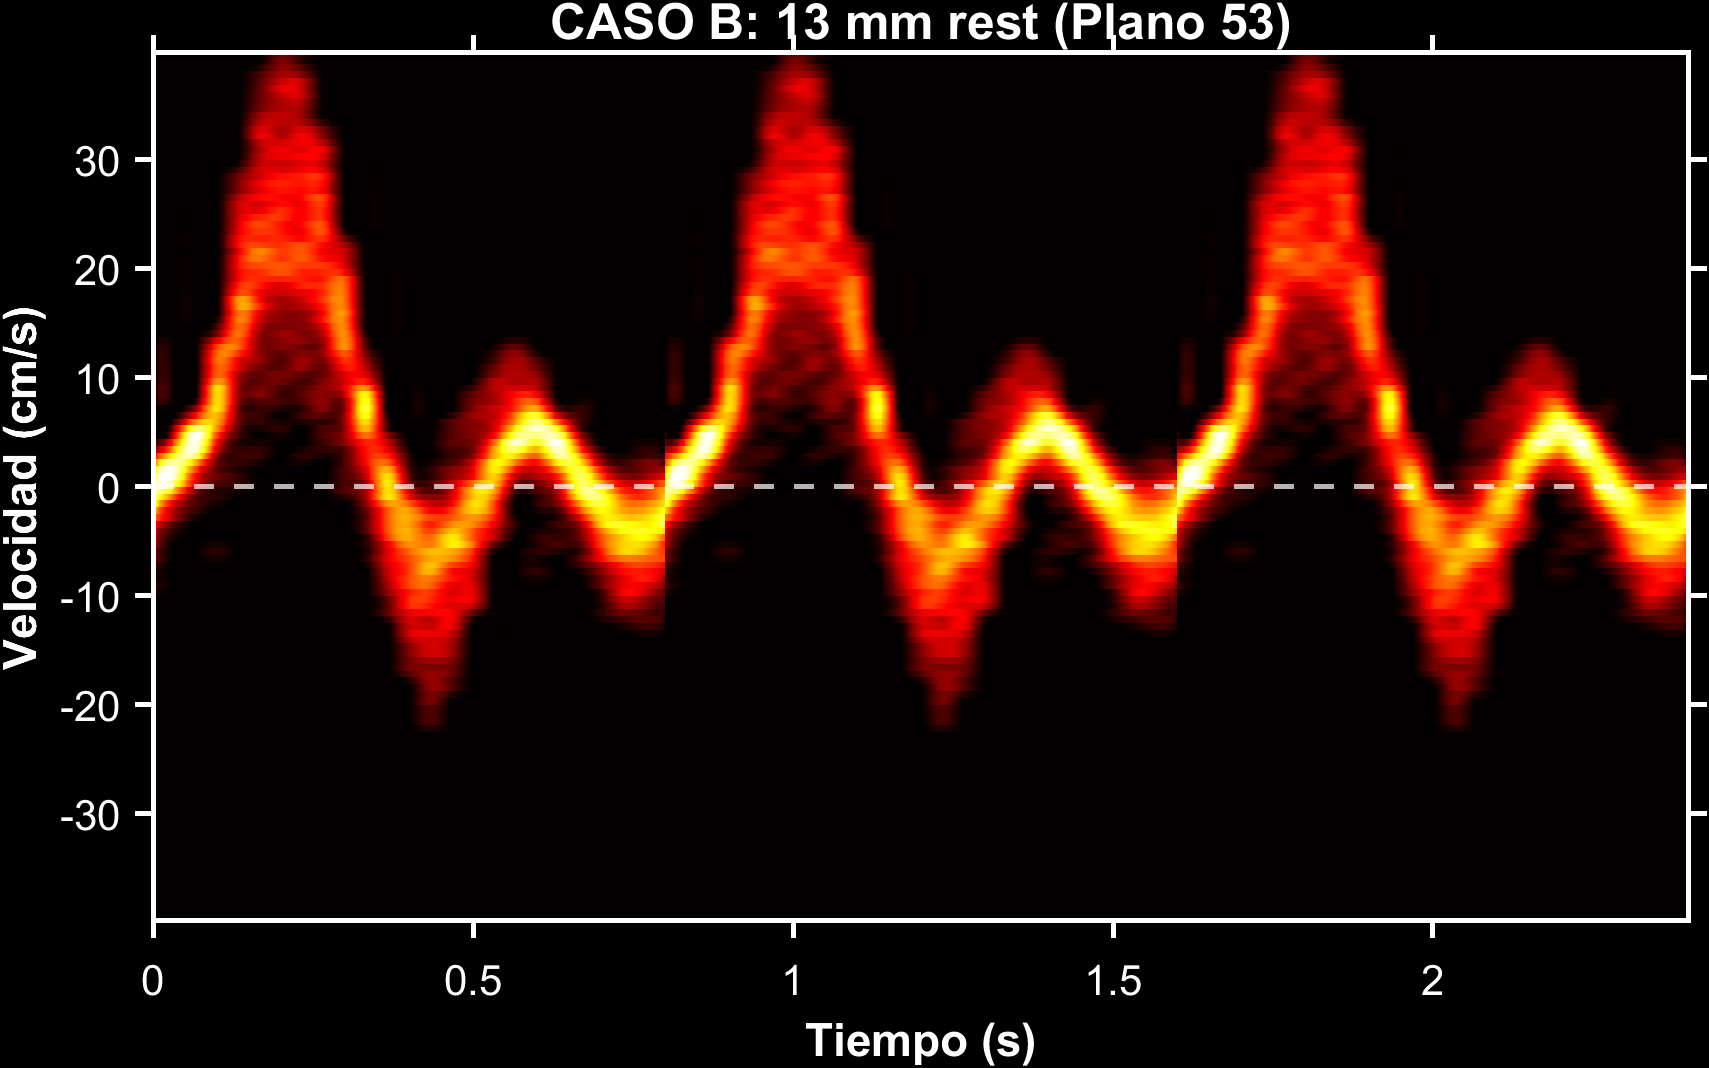
\includegraphics[width=\linewidth]{figures/anexos/13_mm_rest_Plano53.png}
            \caption{\href{https://drive.google.com/file/d/13ViBrWH2iWedRAWQrjs2DRwnu1cg7DFN/view?usp=sharing}{Fantoma 13 mm \textbf{(Escuchar)}}}
            \label{fig:anexo_p53_13mm}
        \end{subfigure}
        
        \vspace{0.4cm}
        
        \begin{subfigure}{0.48\linewidth}
            \centering
            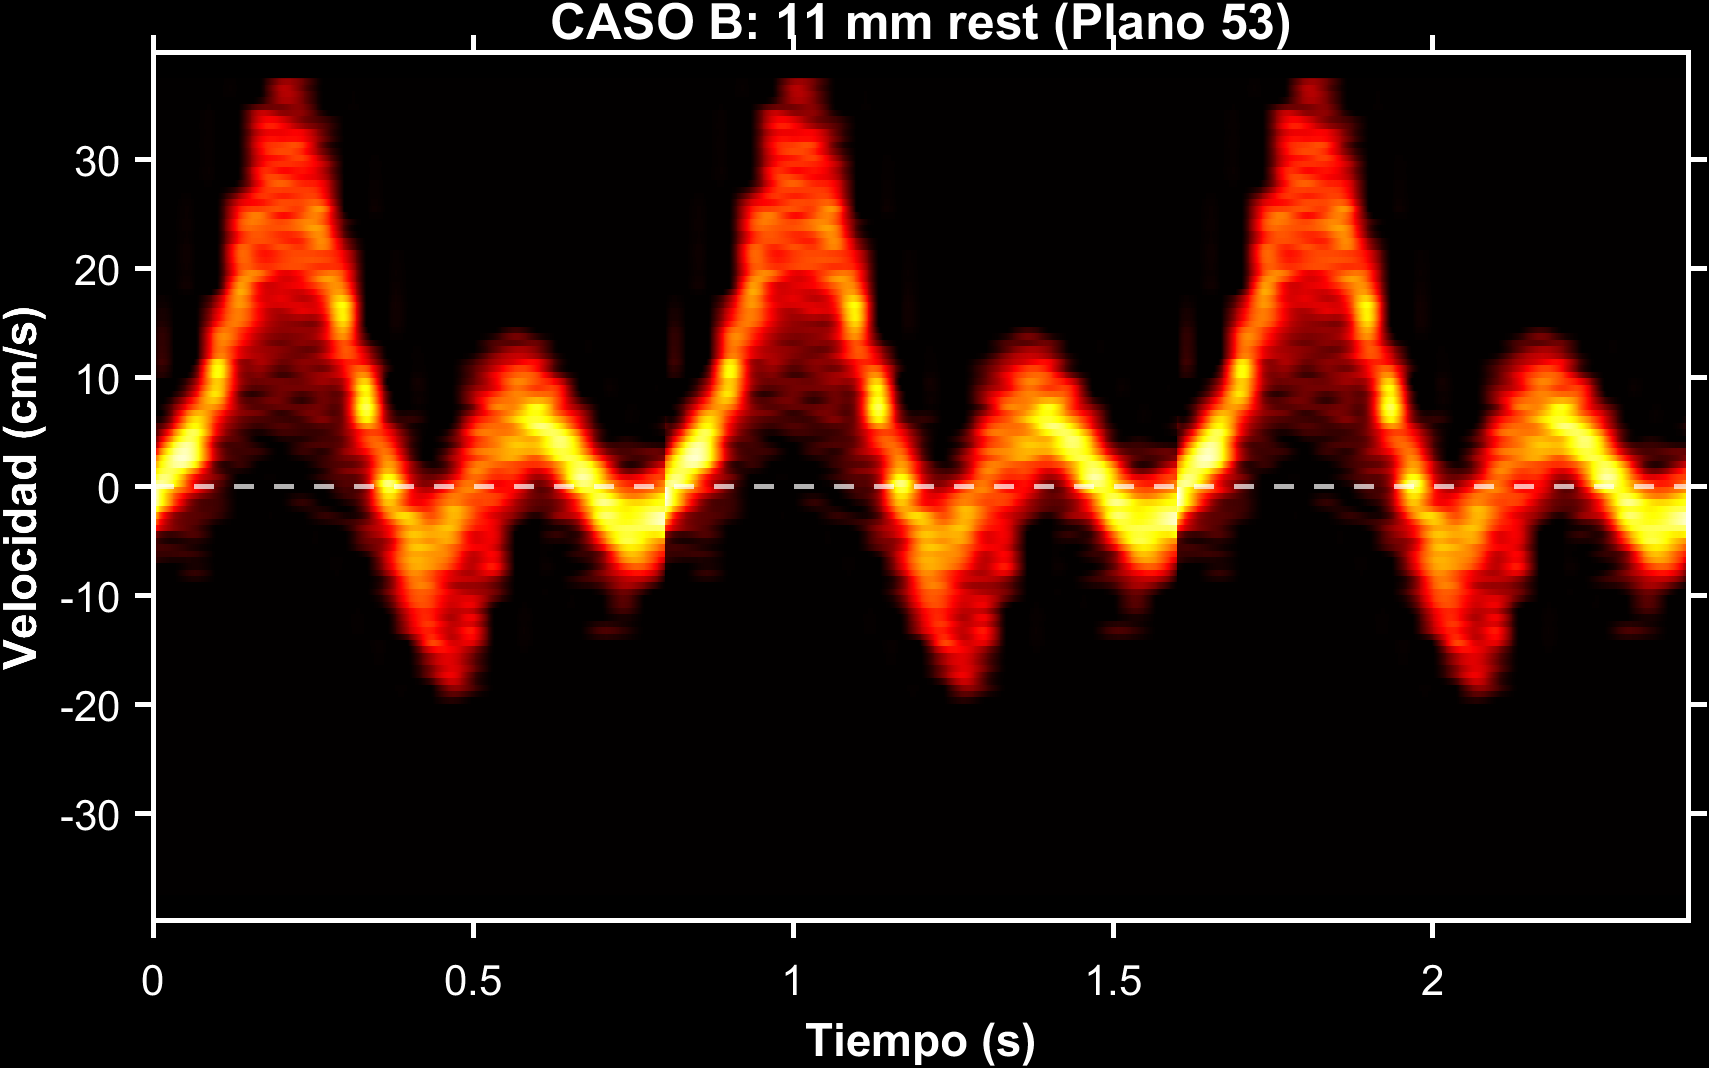
\includegraphics[width=\linewidth]{figures/anexos/11_mm_rest_Plano53.png}
            \caption{\href{https://drive.google.com/file/d/1gsotKFrU7cHhEvFR5qXwZjdcTrV017aL/view?usp=sharing}{Fantoma 11 mm \textbf{(Escuchar)}}}
            \label{fig:anexo_p53_11mm}
        \end{subfigure}\hfill
        \begin{subfigure}{0.48\linewidth}
            \centering
            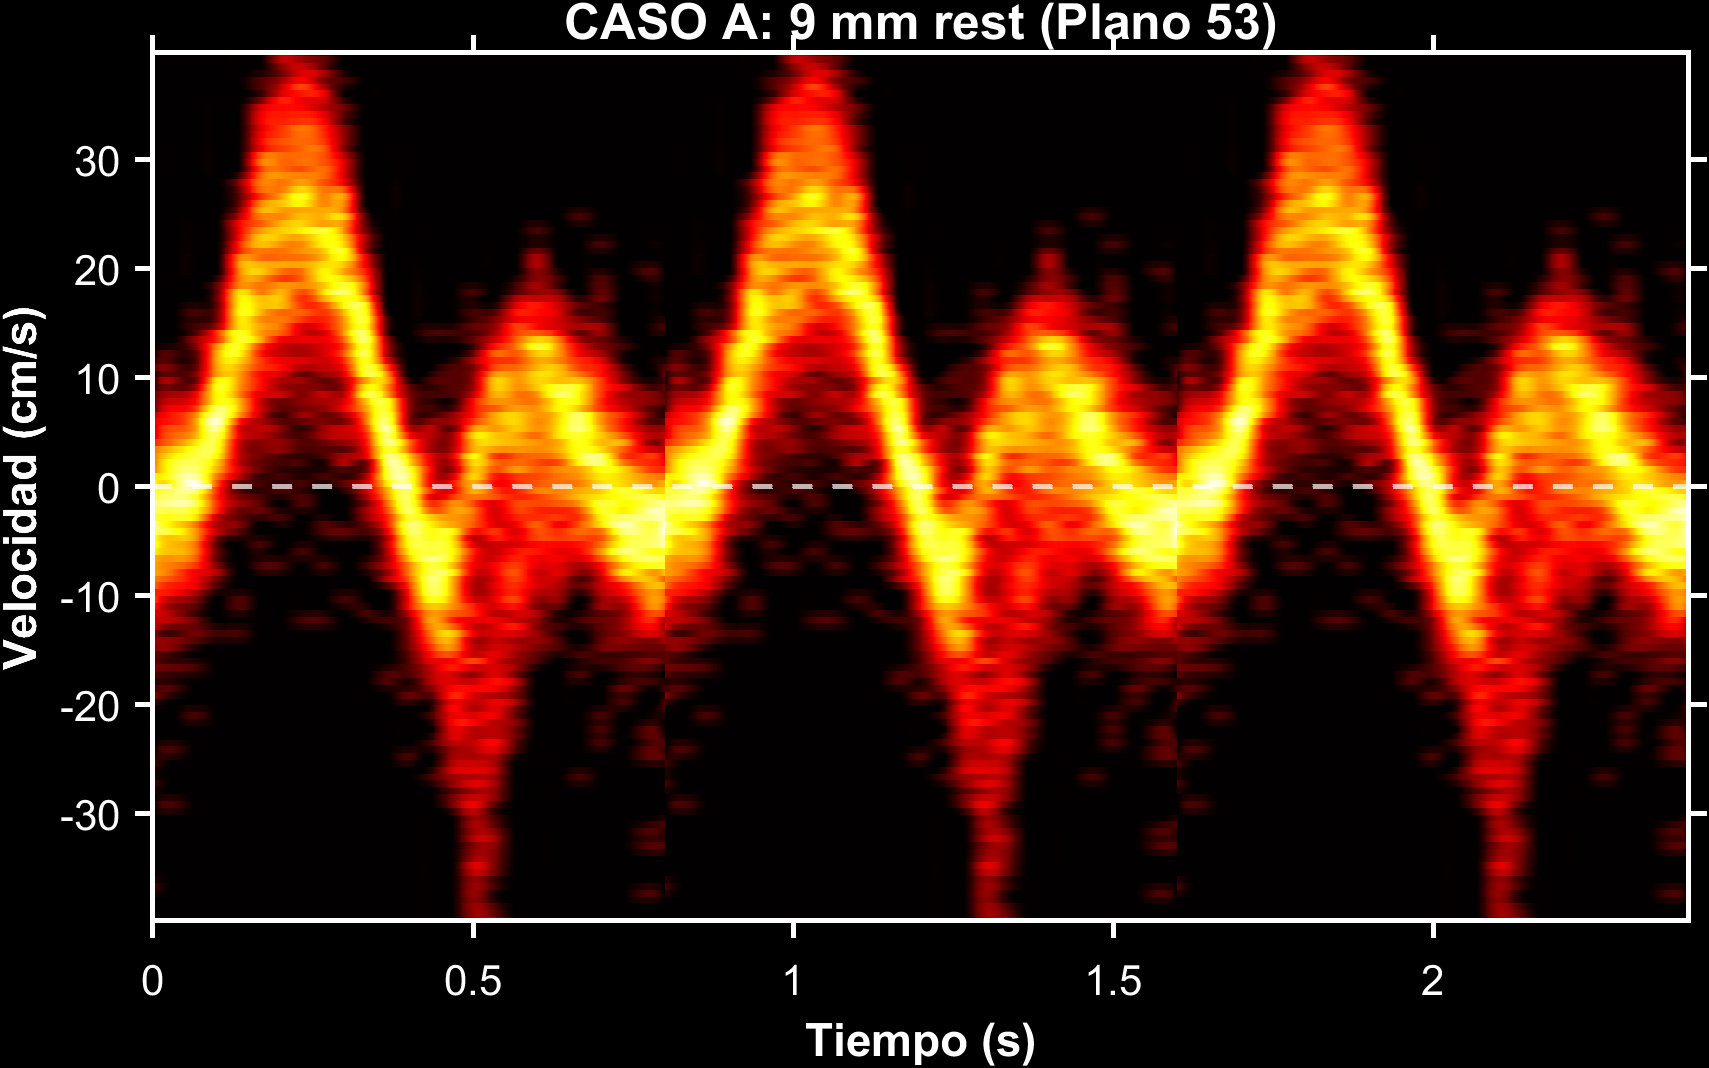
\includegraphics[width=\linewidth]{figures/anexos/9_mm_rest_Plano53.png}
            \caption{\href{https://drive.google.com/file/d/1iDhg9IqTgnRclAD8EpGDnmnlDcU6DA5I/view?usp=sharing}{Fantoma 9 mm \textbf{(Escuchar)}}}
            \label{fig:anexo_p53_9mm}
        \end{subfigure}
    \end{minipage}
    \caption{\label{fig:anexo_comparacion_p53} Evolución espectral en la zona pre-coartación bajo condición de reposo. Fuente: Elaboración propia.}
\end{figure}


\subsection{Análisis comparativo: Post-coartación (plano 70)}

\begin{figure}[H]
    \centering
    \begin{minipage}{0.75\textwidth}
        \begin{subfigure}{0.48\linewidth}
            \centering
            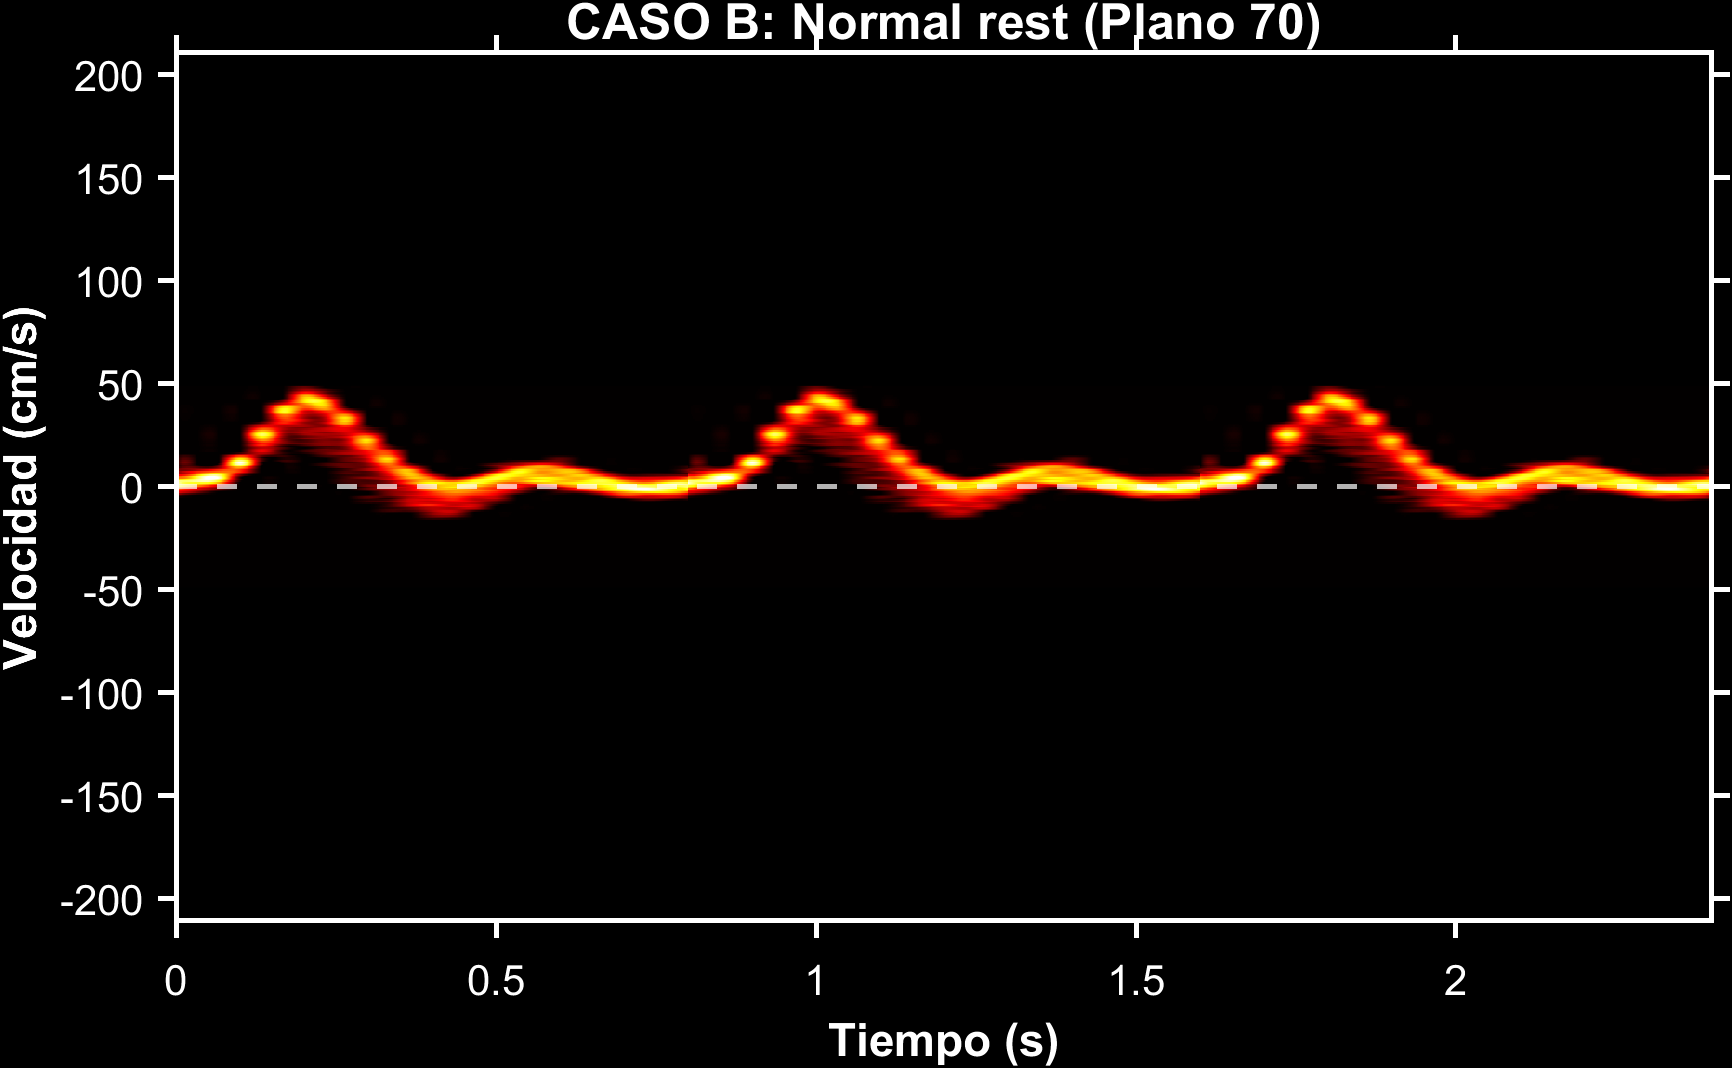
\includegraphics[width=\linewidth]{figures/anexos/Normal_rest_Plano70.png}
            \caption{\href{https://drive.google.com/file/d/1Ji-aclVUsA0XJH64ZcgiSzRloFJDtPAL/view?usp=sharing}{Fantoma normal \textbf{(Escuchar)}}}
            \label{fig:anexo_p70_normal}
        \end{subfigure}\hfill
        \begin{subfigure}{0.48\linewidth}
            \centering
            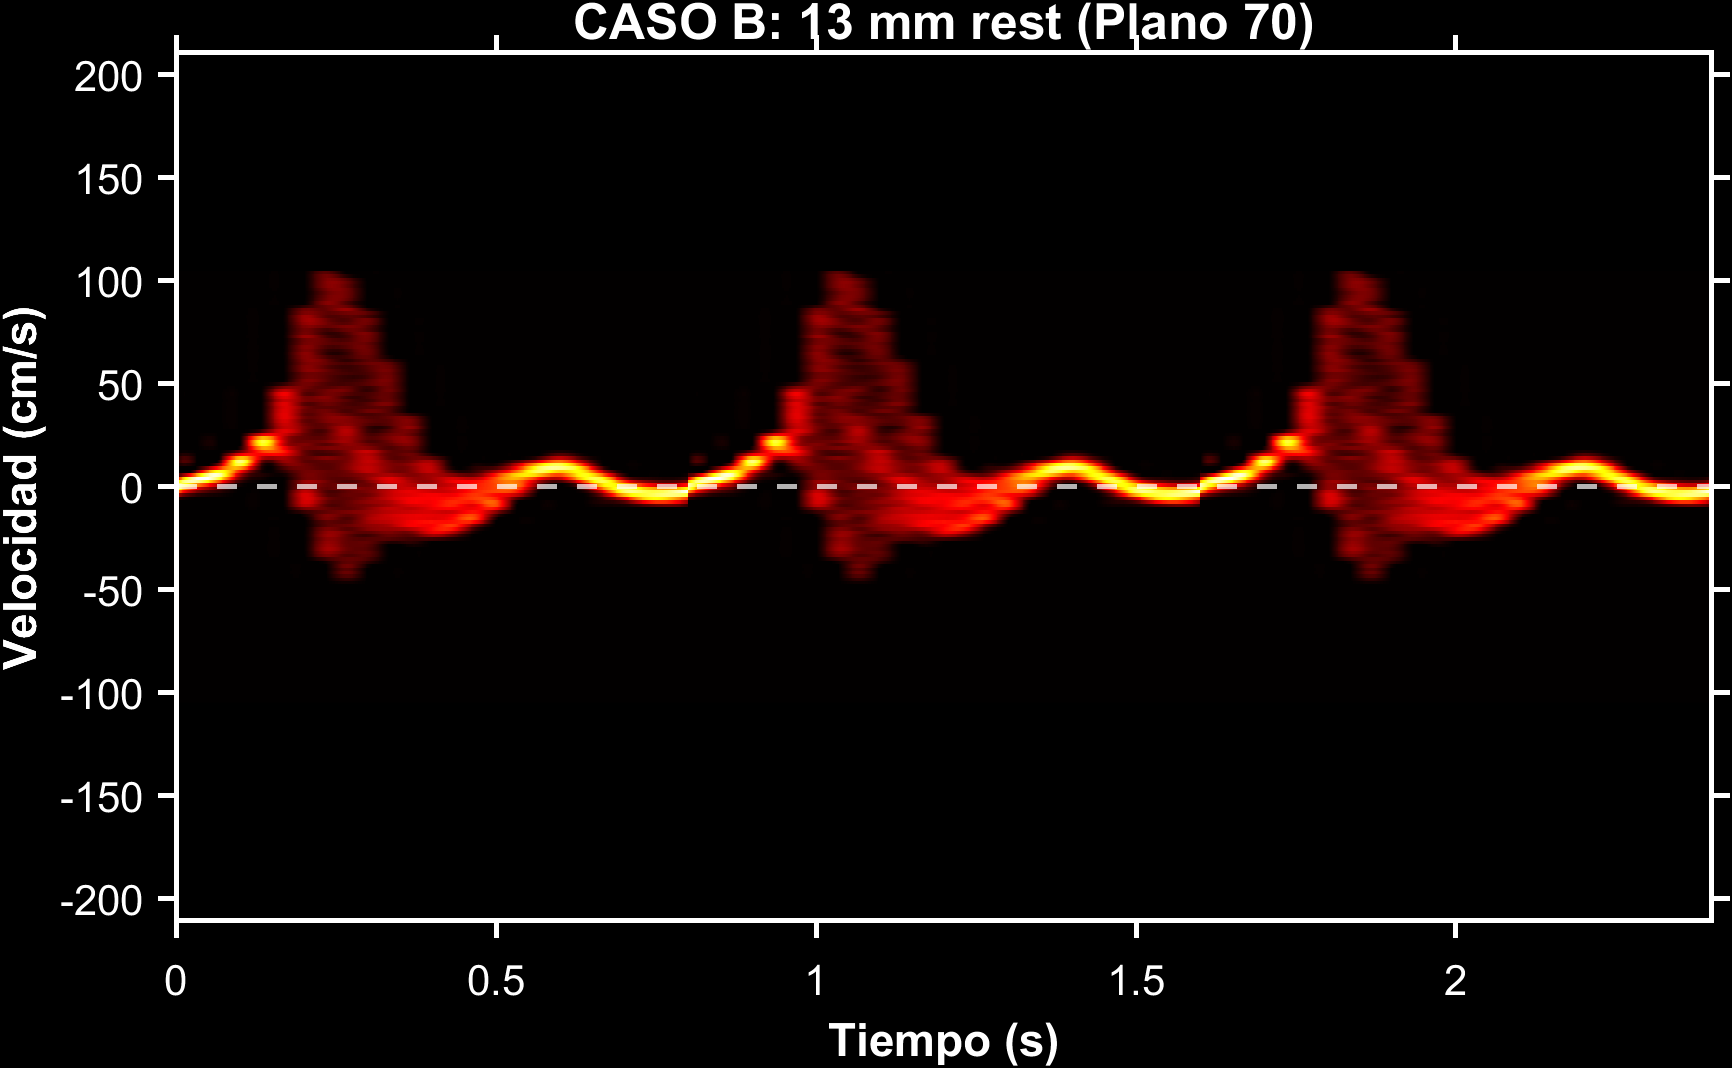
\includegraphics[width=\linewidth]{figures/anexos/13_mm_rest_Plano70.png}
            \caption{\href{https://drive.google.com/file/d/1BXh4fTabW4XNHS3mBkfjZjcfltDJDK9o/view?usp=sharing}{Fantoma 13 mm \textbf{(Escuchar)}}}
            \label{fig:anexo_p70_13mm}
        \end{subfigure}
        
        \vspace{0.4cm}
        
        \begin{subfigure}{0.48\linewidth}
            \centering
            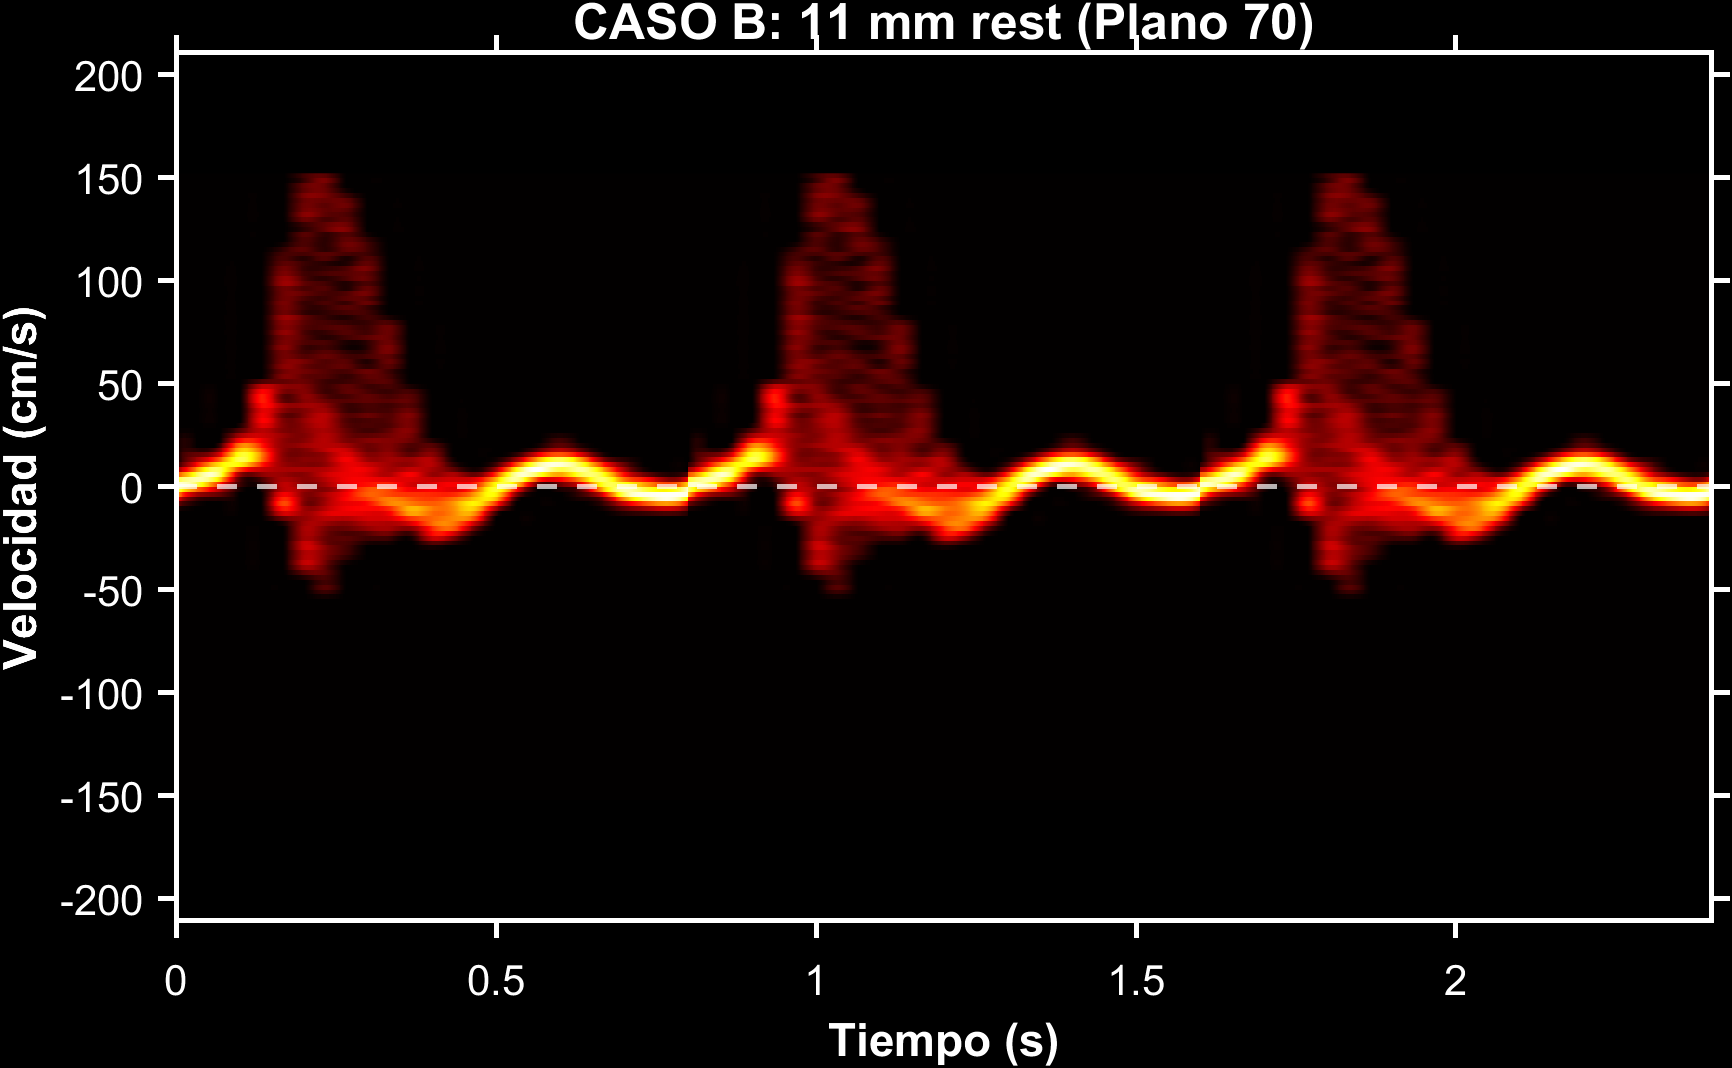
\includegraphics[width=\linewidth]{figures/anexos/11_mm_rest_Plano70.png}
            \caption{\href{https://drive.google.com/file/d/1vKdsexjQyZKzabsV51s44r13G063QVPx/view?usp=sharing}{Fantoma 11 mm \textbf{(Escuchar)}}}
            \label{fig:anexo_p70_11mm}
        \end{subfigure}\hfill
        \begin{subfigure}{0.48\linewidth}
            \centering
            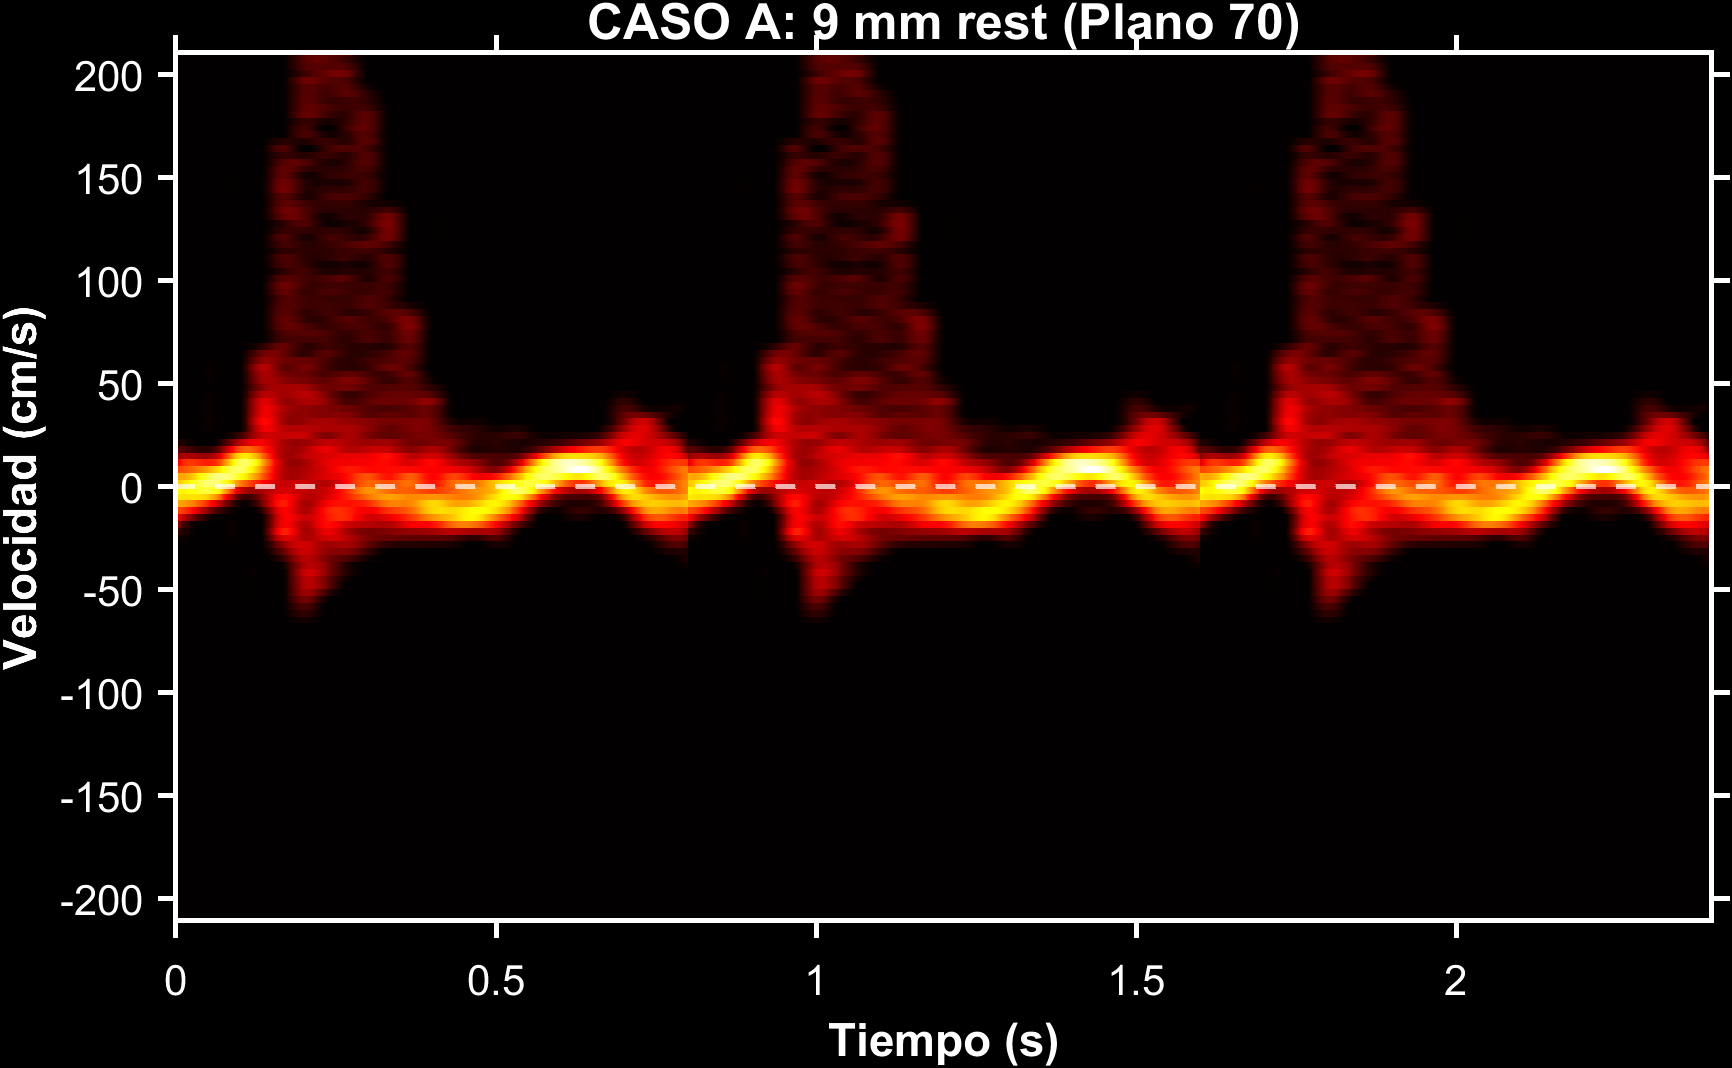
\includegraphics[width=\linewidth]{figures/anexos/9_mm_rest_Plano70.png}
            \caption{\href{https://drive.google.com/file/d/1aBgqeoV4qCd36aoZfs8mPQ5ol-GI3i1W/view?usp=sharing}{Fantoma 9 mm \textbf{(Escuchar)}}}
            \label{fig:anexo_p70_9mm}
        \end{subfigure}
    \end{minipage}
    \caption{\label{fig:anexo_comparacion_p70} Evolución espectral en la zona post-coartación bajo condición de reposo. Fuente: Elaboración propia.}
\end{figure}

\section{Exploración de los casos borde}
\label{anexo:casos_borde}
En este anexo se presentan los casos borde de la segmentacion. Se incluyen las condiciones de reposo y estrés, para los fantomas normal y 9 mm. Para mantener la coherencia se presentan la geometría asociada y los diferentes planos.

\begin{figure}[H]
    \centering
    \begin{minipage}{0.75\textwidth}
        \begin{subfigure}{0.48\linewidth}
            \centering
            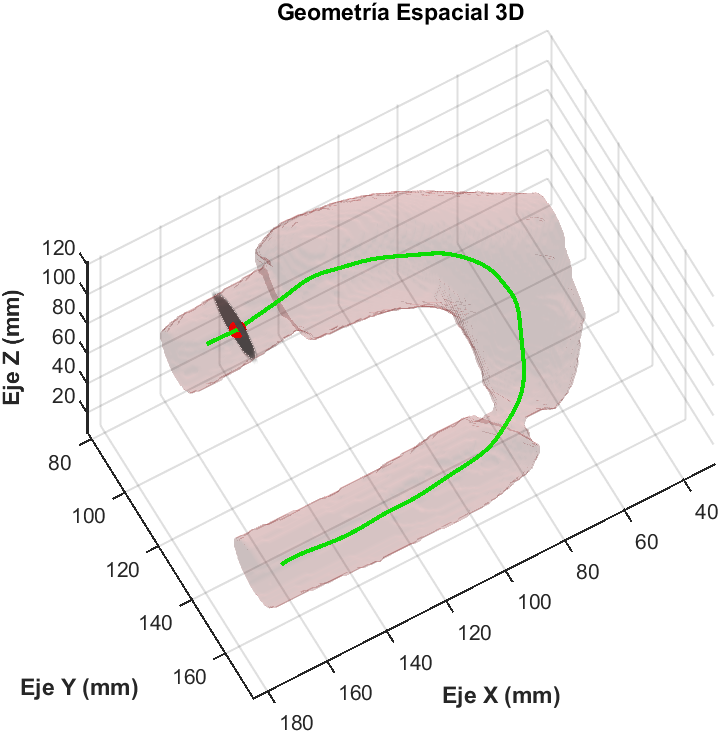
\includegraphics[width=\linewidth]{figures/anexos/9mm_plano5.png}
            \caption{Plano 5 (aorta ascendente proximal)}
            \label{fig:anexo_geo_p5}
        \end{subfigure}\hfill
        \begin{subfigure}{0.48\linewidth}
            \centering
            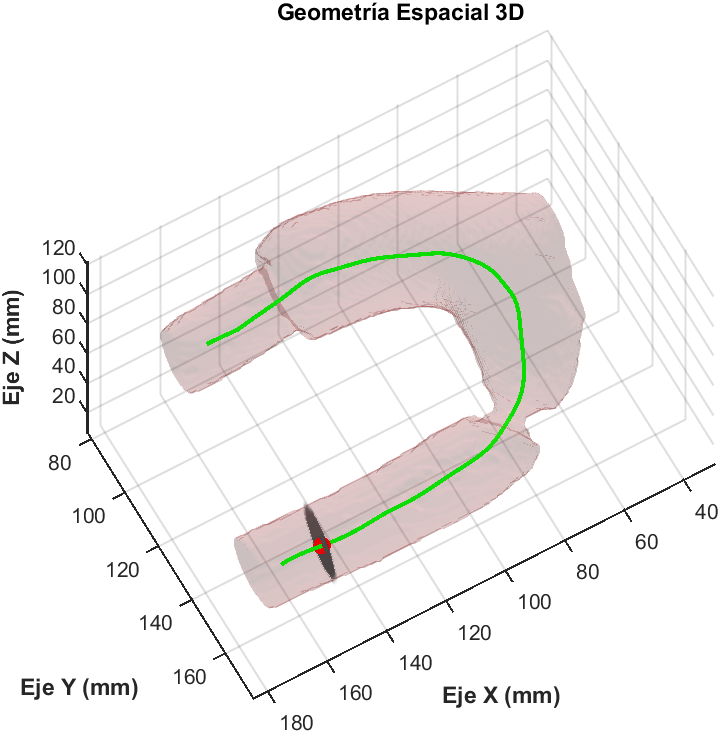
\includegraphics[width=\linewidth]{figures/anexos/9mm_plano85.png}
            \caption{Plano 85 (aorta descendente distal)}
            \label{fig:anexo_geo_p85}
        \end{subfigure}
    \end{minipage}
    \caption{\label{fig:anexo_geometria_extremos} Representación tridimensional del fantoma de 9mm. Ilustra la ubicación de los planos en los casos borde. La línea verde representa el \textit{centerline}. Fuente: Elaboración propia.}
\end{figure}

\subsection{Análisis comparativo extremo: Plano 5}

\begin{figure}[H]
    \centering
    \begin{minipage}{0.75\textwidth}
        \begin{subfigure}{0.48\linewidth}
            \centering
            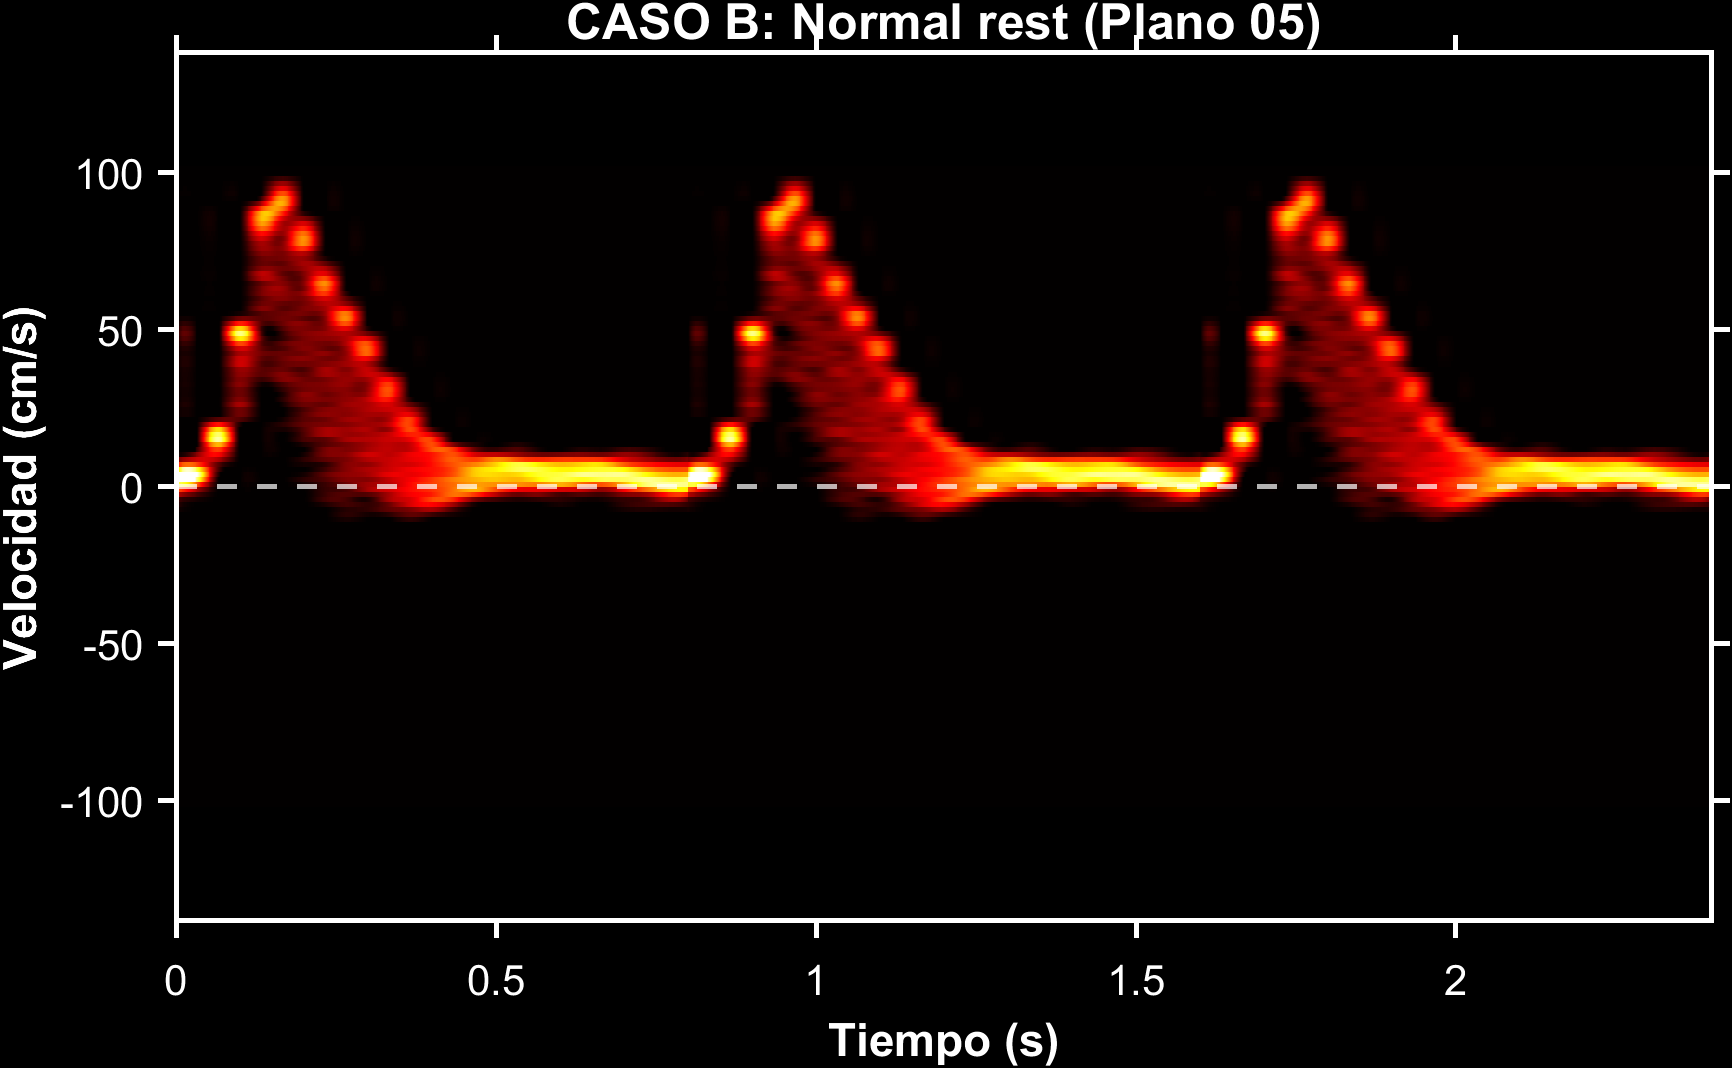
\includegraphics[width=\linewidth]{figures/anexos/Normal_rest_Plano05.png}
            \caption{\href{https://drive.google.com/file/d/1YK31lfkGaEXx60OxTx7NMA_Cw63nC900/view?usp=sharing}{Normal \textit{rest} \textbf{(Escuchar)}}}
            \label{fig:anexo_p5_normal_rest}
        \end{subfigure}\hfill
        \begin{subfigure}{0.48\linewidth}
            \centering
            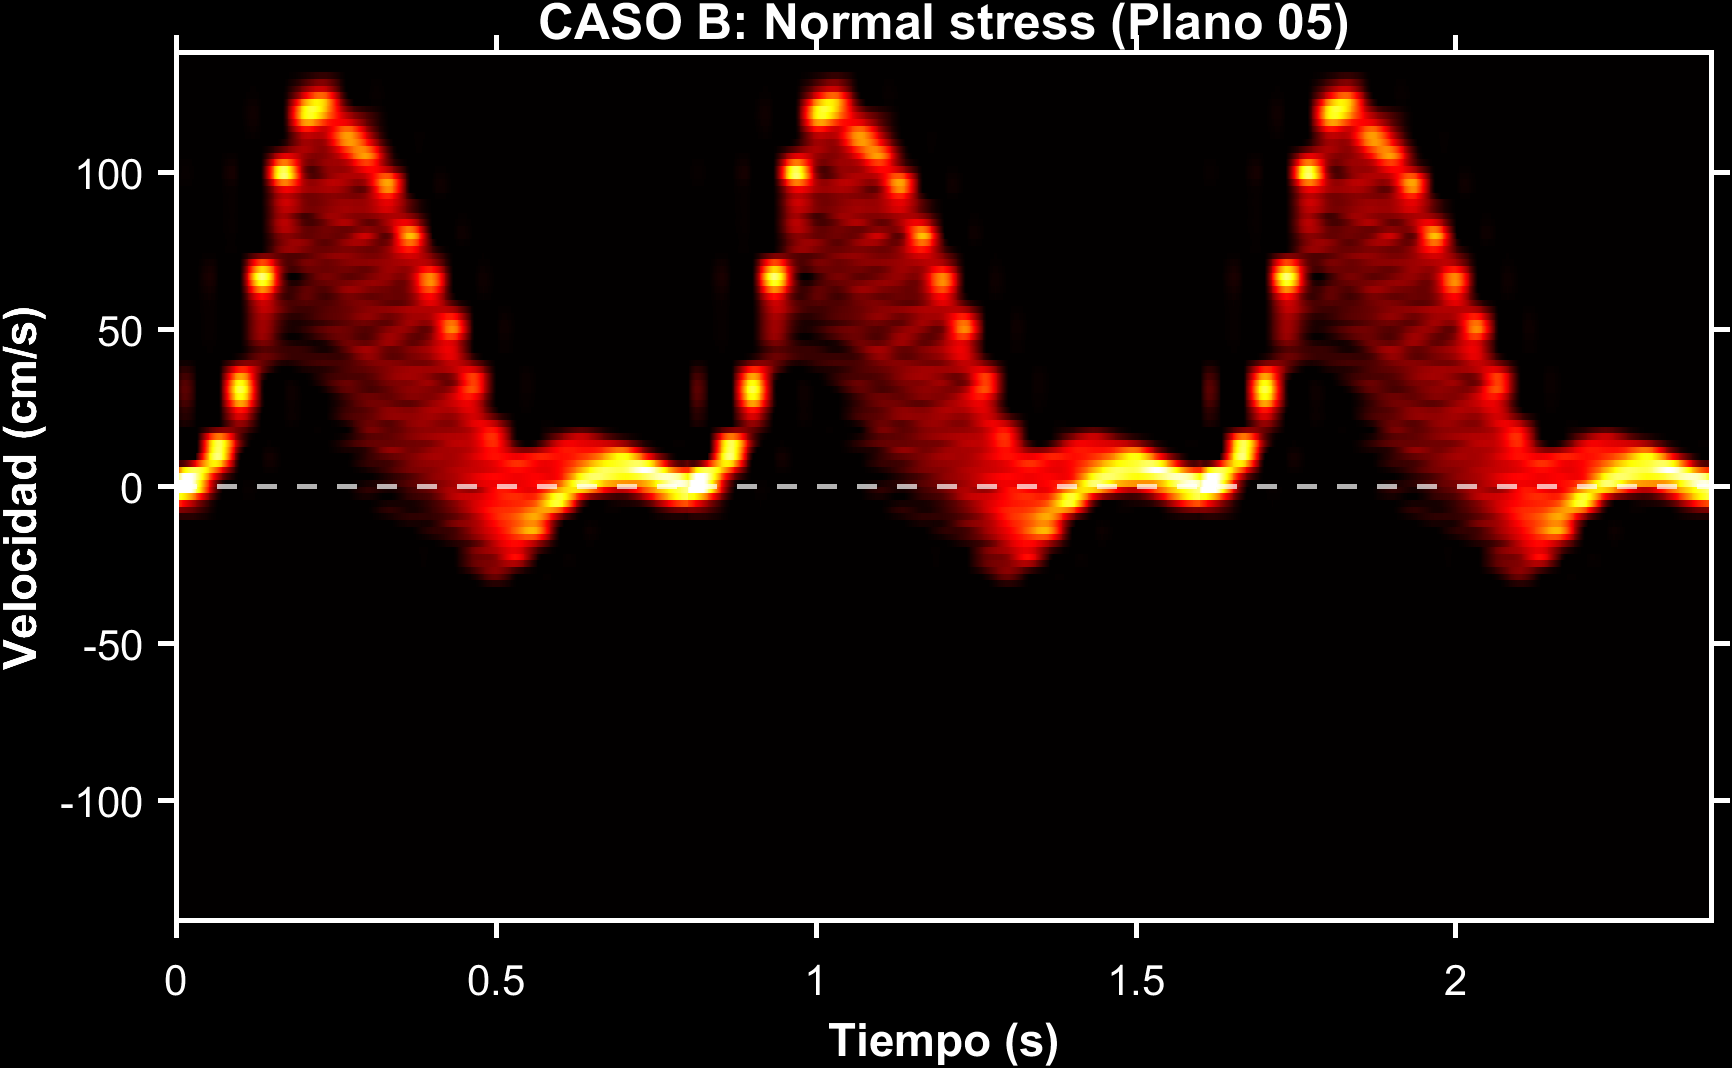
\includegraphics[width=\linewidth]{figures/anexos/Normal_stress_Plano05.png}
            \caption{\href{https://drive.google.com/file/d/1YZu0HmBU-EFEgWmTePQ66v50J-19i2o7/view?usp=sharing}{Normal \textit{stress} \textbf{(Escuchar)}}}
            \label{fig:anexo_p5_normal_stress}
        \end{subfigure}
        
        \vspace{0.4cm}
        
        \begin{subfigure}{0.48\linewidth}
            \centering
            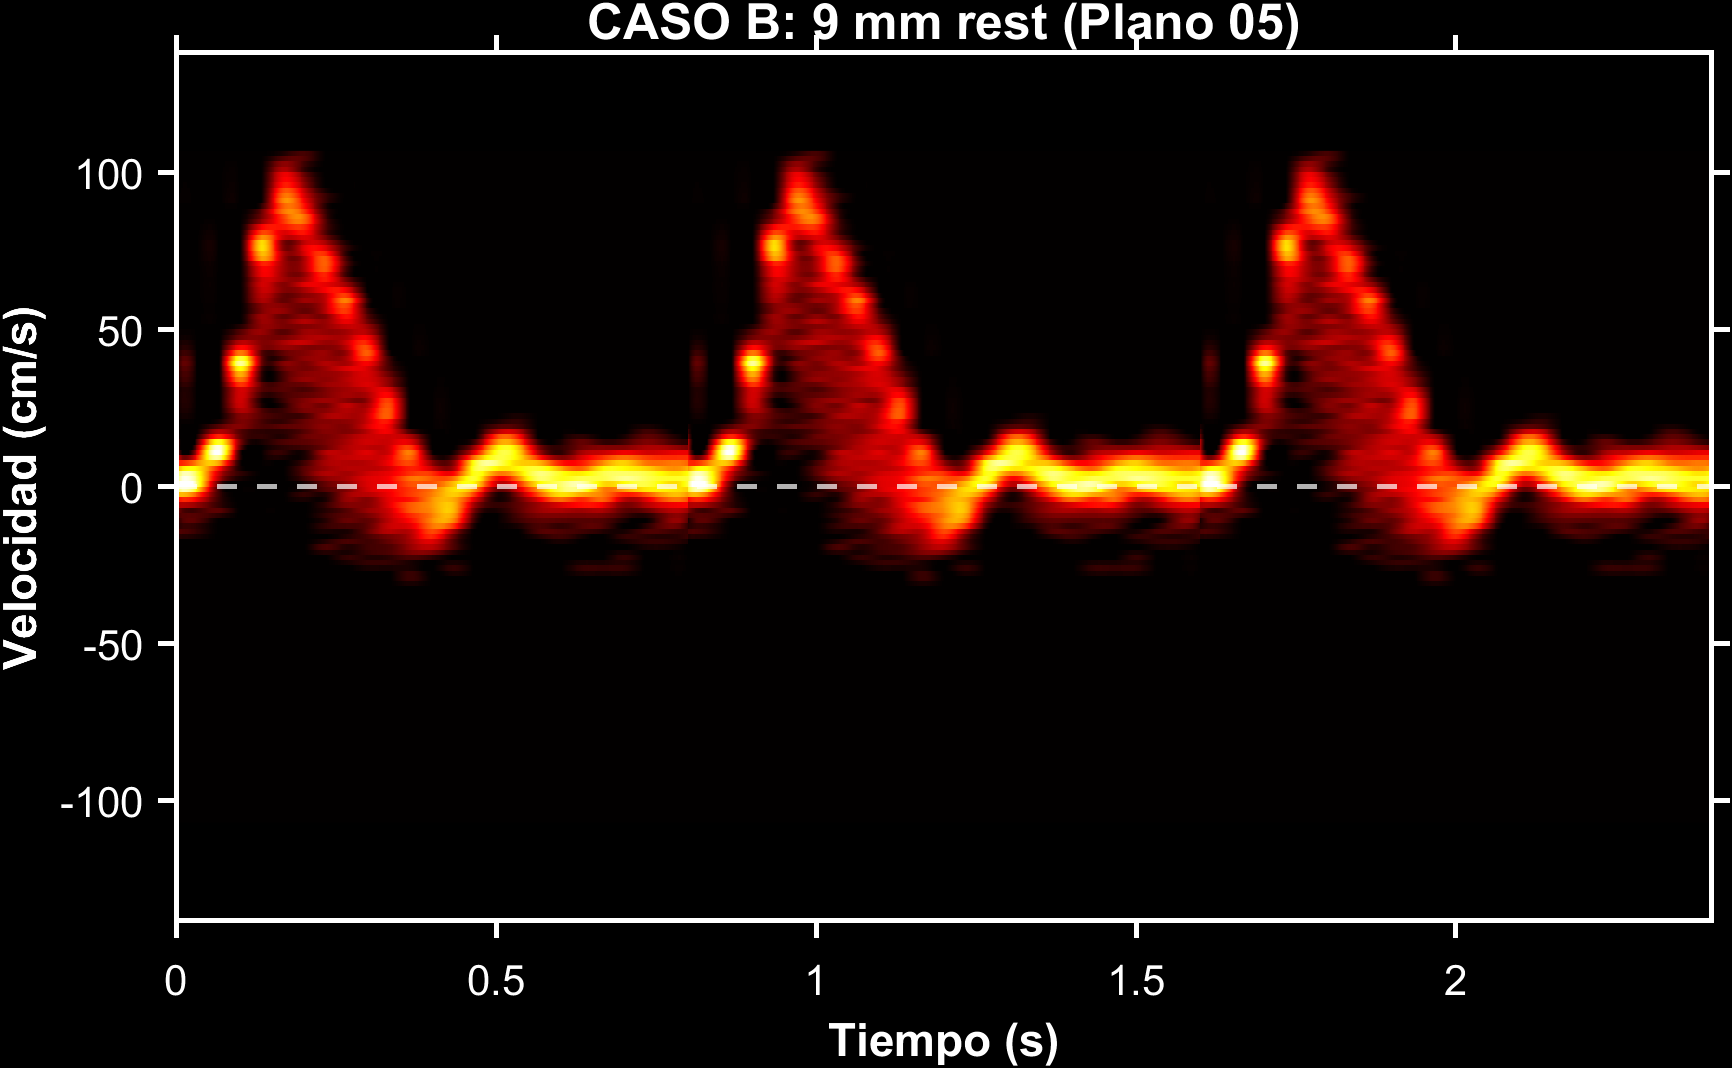
\includegraphics[width=\linewidth]{figures/anexos/9_mm_rest_Plano05.png}
            \caption{\href{https://drive.google.com/file/d/15aY5Ka3epcruwTPN9ZXKztg4-zE6n9DE/view?usp=sharing}{9 mm \textit{rest} \textbf{(Escuchar)}}}
            \label{fig:anexo_p5_9mm_rest}
        \end{subfigure}\hfill
        \begin{subfigure}{0.48\linewidth}
            \centering
            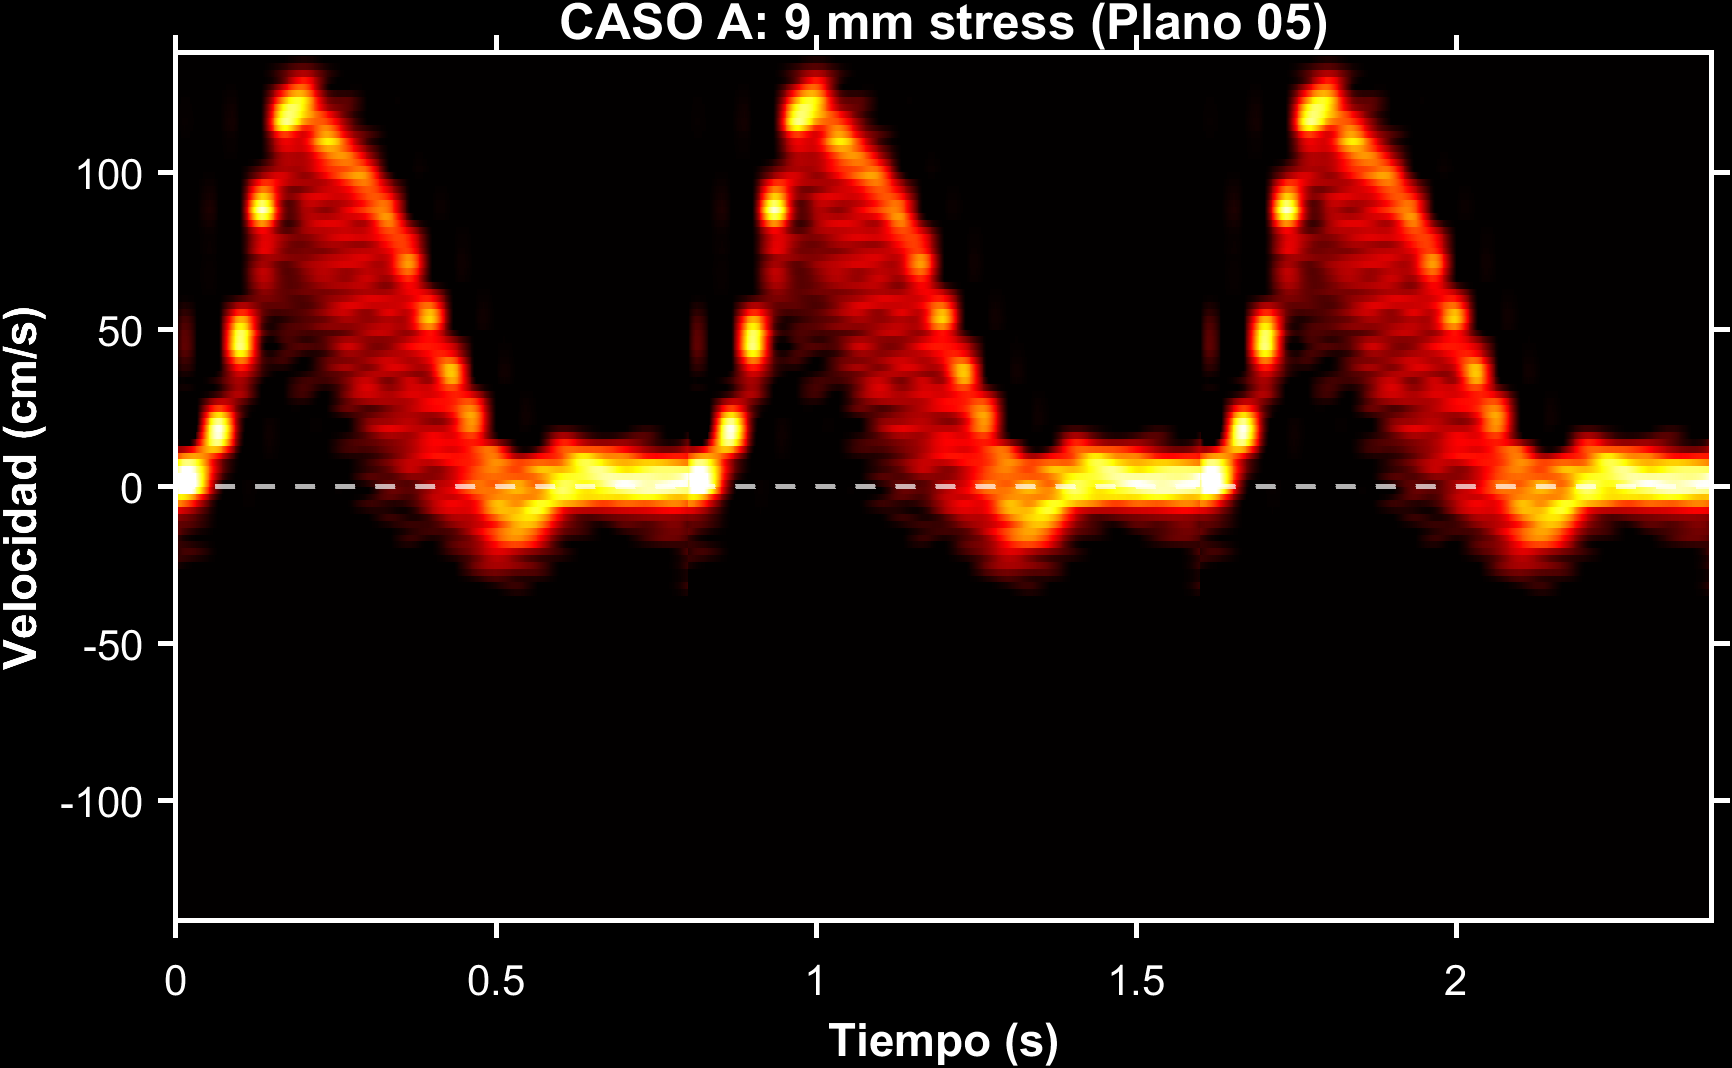
\includegraphics[width=\linewidth]{figures/anexos/9_mm_stress_Plano05.png}
            \caption{\href{https://drive.google.com/file/d/1KWstZDt0APd1gukMKM52vnXZ9ZMmdCZZ/view?usp=sharing}{9 mm \textit{stress} \textbf{(Escuchar)}}}
            \label{fig:anexo_p5_9mm_stress}
        \end{subfigure}
    \end{minipage}
    \caption{\label{fig:anexo_comparacion_p5} Comparación espectral en el plano 5 evaluando los casos Normal y 9 mm bajo condiciones de reposo y estrés. Fuente: Elaboración propia.}
\end{figure}


\subsection{Análisis comparativo extremo: Plano 85}

\begin{figure}[H]
    \centering
    \begin{minipage}{0.75\textwidth}
        \begin{subfigure}{0.48\linewidth}
            \centering
            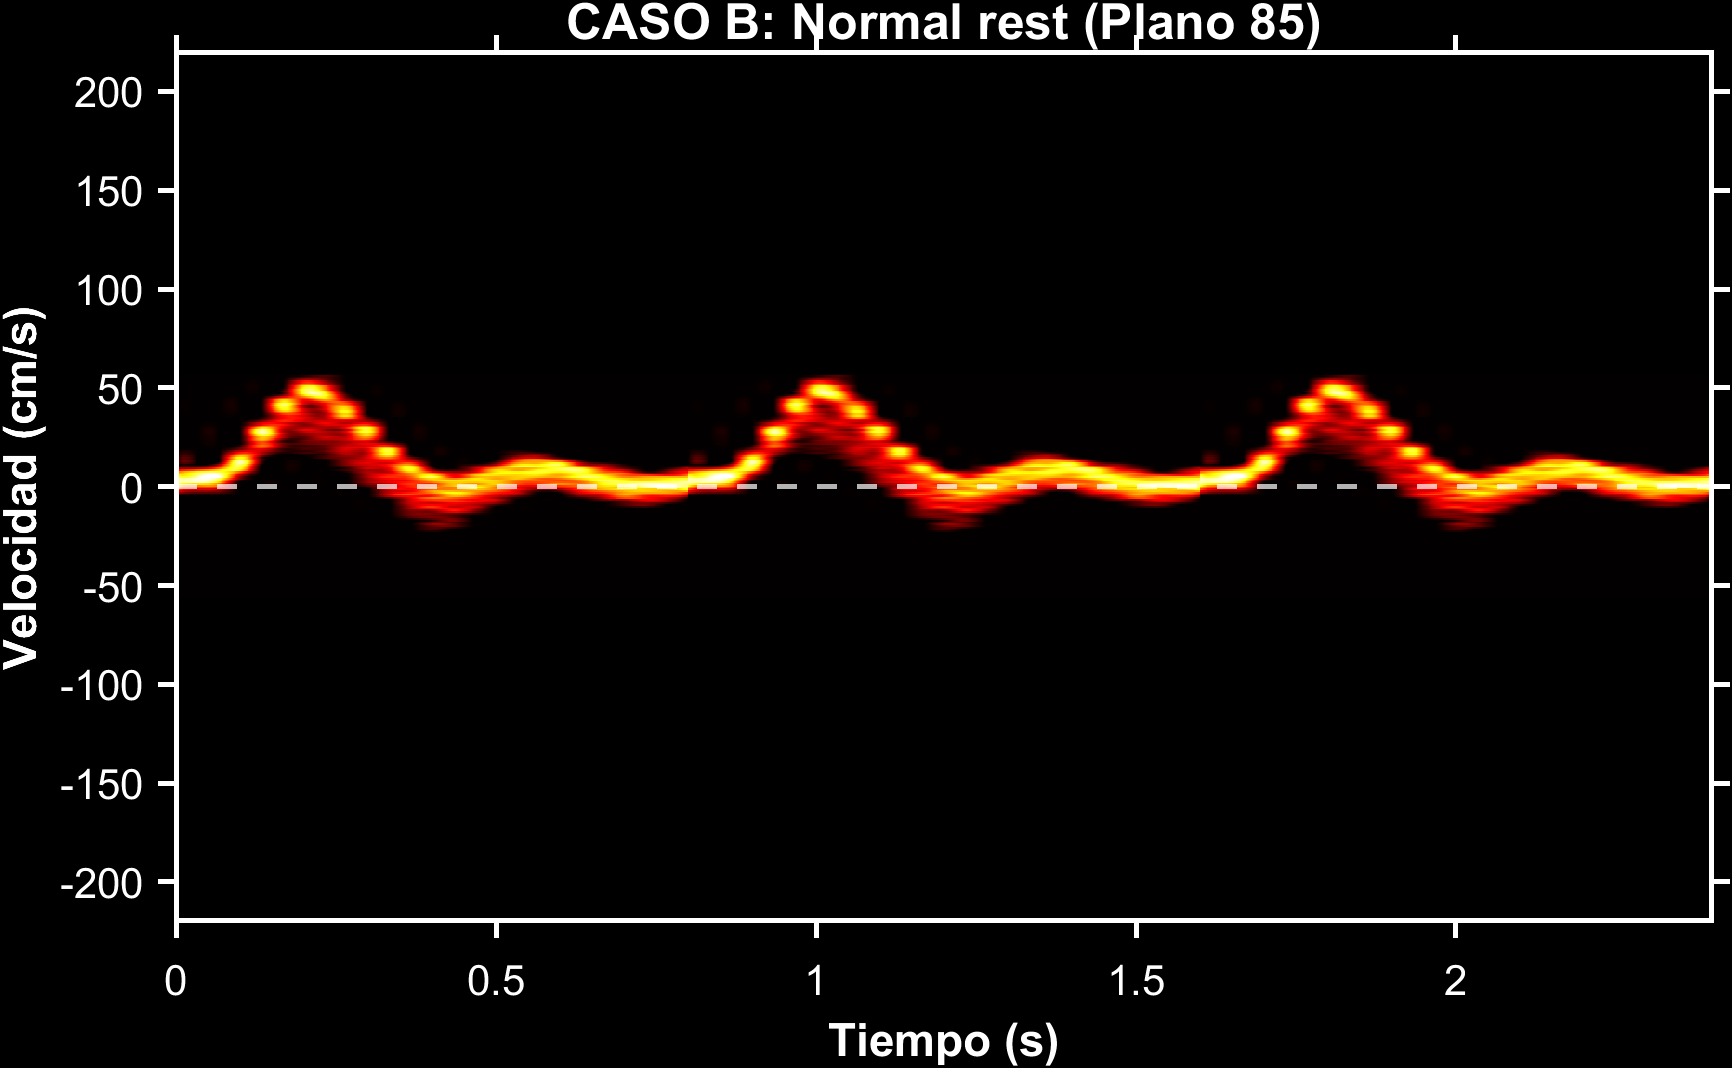
\includegraphics[width=\linewidth]{figures/anexos/Normal_rest_Plano85.png}
            \caption{\href{https://drive.google.com/file/d/1x_aCgRlC-U291iP3yWYODxnAIjABdu7s/view?usp=sharing}{Normal \textit{rest} \textbf{(Escuchar)}}}
            \label{fig:anexo_p85_normal_rest}
        \end{subfigure}\hfill
        \begin{subfigure}{0.48\linewidth}
            \centering
            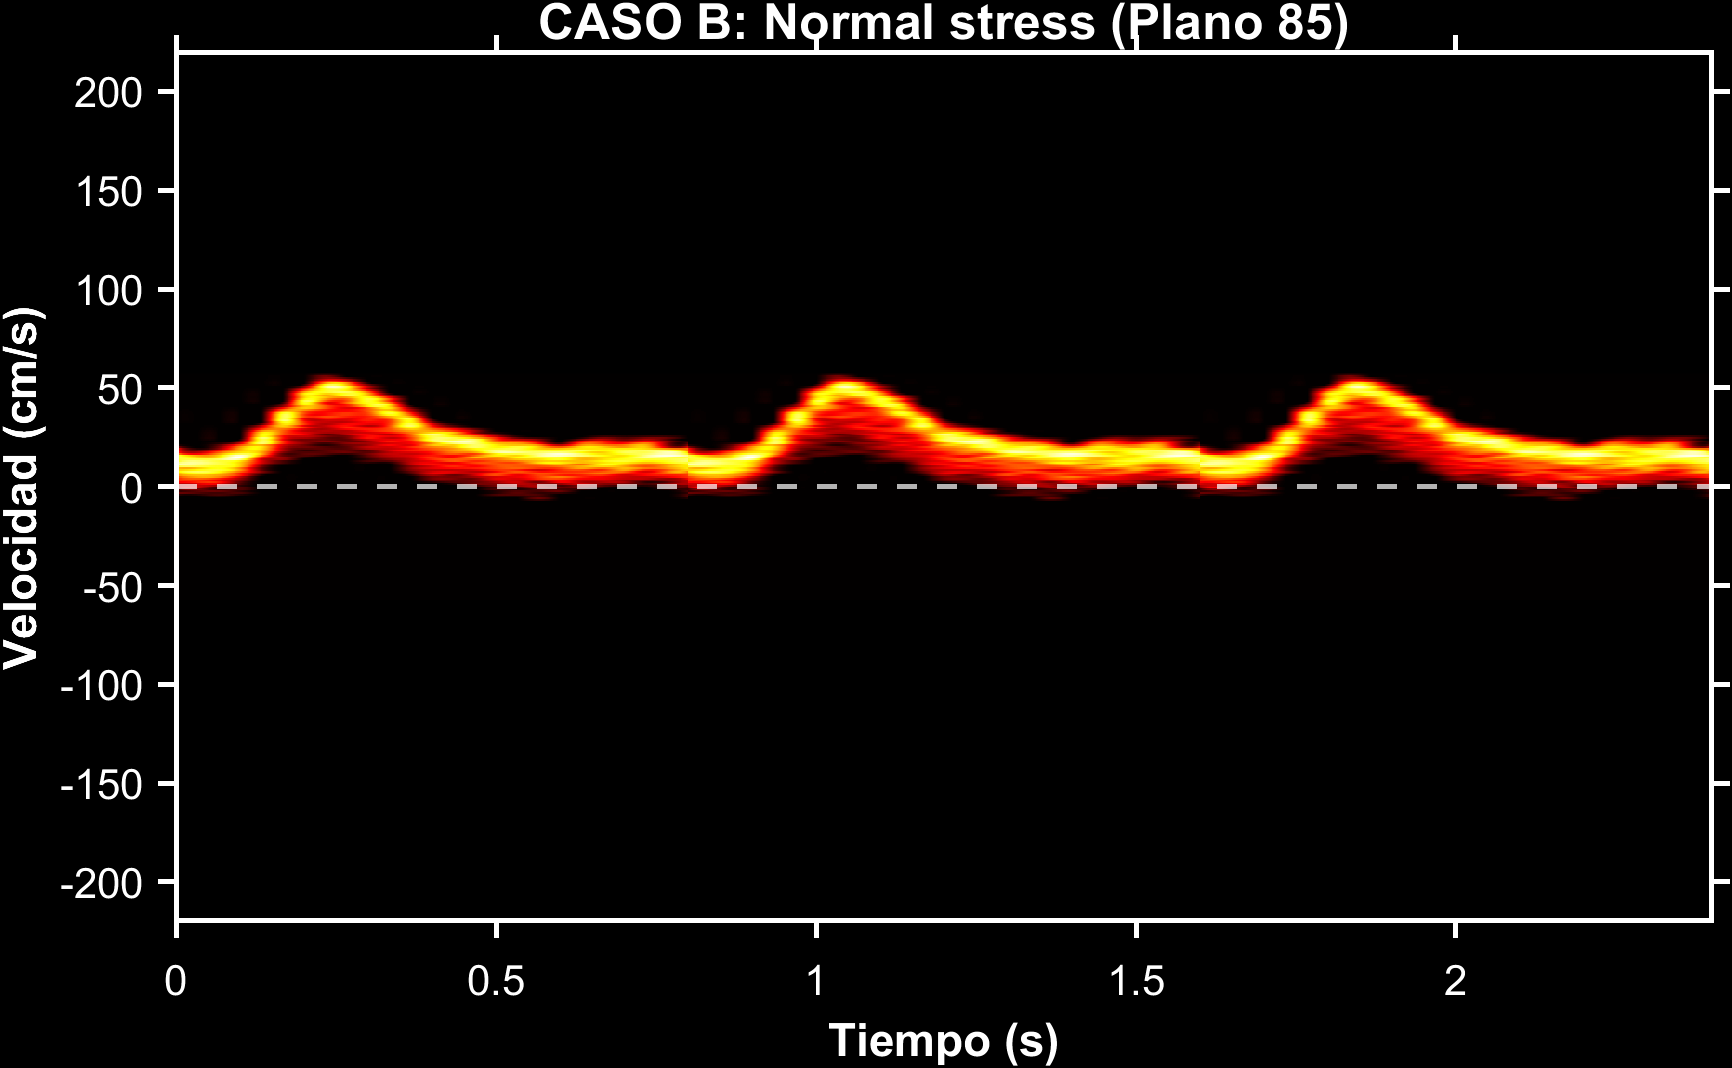
\includegraphics[width=\linewidth]{figures/anexos/Normal_stress_Plano85.png}
            \caption{\href{https://drive.google.com/file/d/1ZpgR28frecUy7BBZH10Bbx4weVoIk4Ci/view?usp=sharing}{Normal \textit{stress} \textbf{(Escuchar)}}}
            \label{fig:anexo_p85_normal_stress}
        \end{subfigure}
        
        \vspace{0.4cm}
        
        \begin{subfigure}{0.48\linewidth}
            \centering
            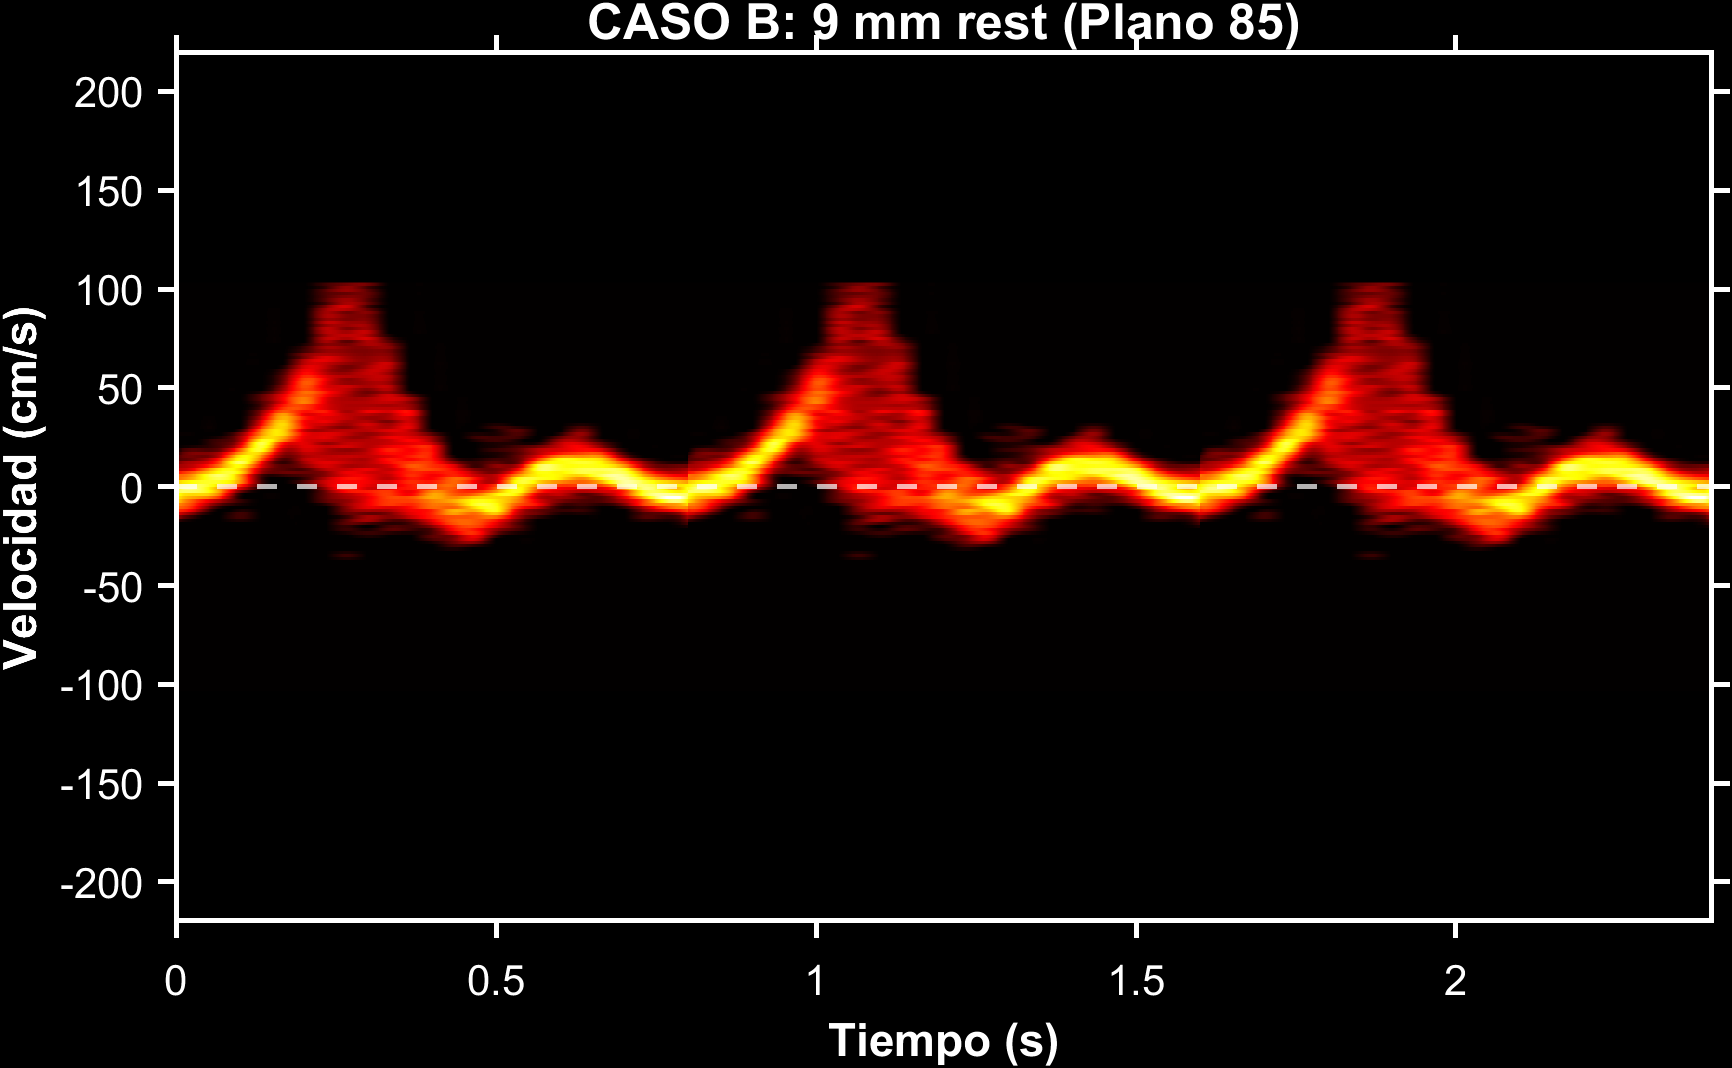
\includegraphics[width=\linewidth]{figures/anexos/9_mm_rest_Plano85.png}
            \caption{\href{https://drive.google.com/file/d/1xdobj-27zKS08QWK1PNRTL2fhcNn9-fd/view?usp=sharing}{9 mm \textit{rest} \textbf{(Escuchar)}}}
            \label{fig:anexo_p85_9mm_rest}
        \end{subfigure}\hfill
        \begin{subfigure}{0.48\linewidth}
            \centering
            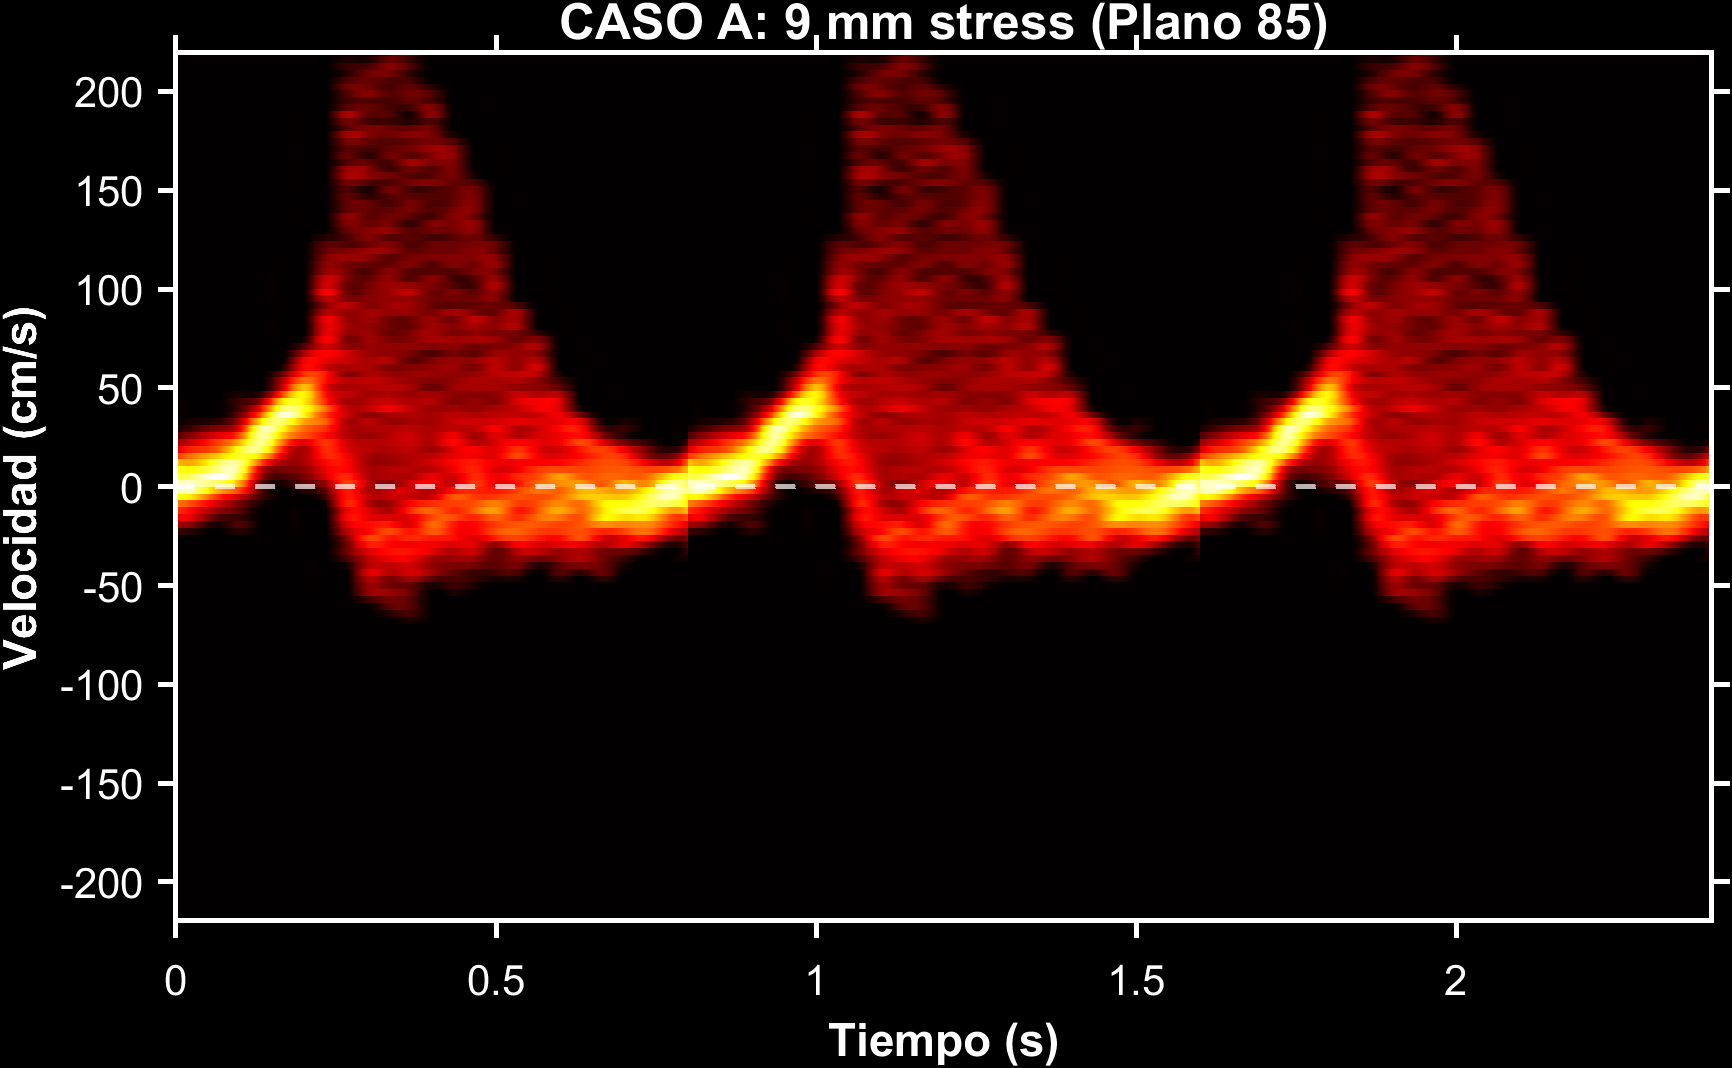
\includegraphics[width=\linewidth]{figures/anexos/9_mm_stress_Plano85.png}
            \caption{\href{https://drive.google.com/file/d/1xdobj-27zKS08QWK1PNRTL2fhcNn9-fd/view?usp=sharing}{9 mm \textit{stress} \textbf{(Escuchar)}}}
            \label{fig:anexo_p85_9mm_stress}
        \end{subfigure}
    \end{minipage}
    \caption{\label{fig:anexo_comparacion_p85} Comparación espectral en el plano 85 evaluando los casos Normal y 9 mm bajo condiciones de reposo y estrés. Fuente: Elaboración propia.}
\end{figure}

\newpage
% Bibliografía estilo APA:
\bibliographystyle{apalike-es}
\bibliography{bibliografia}{}

\end{document}
